%%%%%%%%%%%%%%%%%%%%%%%%%%%%%%%%%%%%%%%%%%%%%%%%%%%%%%%%%%%%%%%%%%%%%%%%%%%%%%%%
%%%%%%%%%%%%%%%%%%%%%%%%%%%%%%%%%%%%%%%%%%%%%%%%%%%%%%%%%%%%%%%%%%%%%%%%%%%%%%%%
%%                           AUTHOR: BIBEKANANDA DATTA                        %%
%%                               (C) MARCH 2024                               %%
%%                      PhD STUDENT, MECHANICAL ENGINEERING                   %%
%%                           JOHNS HOPKINS UNIVERSITY                         %%
%%%%%%%%%%%%%%%%%%%%%%%%%%%%%%%%%%%%%%%%%%%%%%%%%%%%%%%%%%%%%%%%%%%%%%%%%%%%%%%%
%%%%%%%%%%%%%%%%%%%%%%%%%%%%%%%%%%%%%%%%%%%%%%%%%%%%%%%%%%%%%%%%%%%%%%%%%%%%%%%%
%%             PLEASE CHECK THE README.md FILE BEFORE YOU PROCEED             %%
%%              it may be convenient to read this file on GitHub              %%
%%   GitHub: https://github.com/bibekananda-datta/JHU-Dissertation-Template   %%
%% template hosted on this GitHub repository is likely to be the most updated %%
%%%%%%%%%%%%%%%%%%%%%%%%%%%%%%%%%%%%%%%%%%%%%%%%%%%%%%%%%%%%%%%%%%%%%%%%%%%%%%%%

%%%%%%%%%%%%%%%%%%%%%%%%%%%%%%%%%%%%%%%%%%%%%%%%%%%%%%%%%%%%%%%%%%%%%%%%%%%%%%%%
% This is an unofficial dissertation template for Johns Hopkins University.
% As of March 31, 2024, the template follows the dissertation formatting 
% requirements provided by the  Johns Hopkins University Sheridan Library.
% It is the user's responsibility to ensure that the current requirements are 
% followed: https://www.library.jhu.edu/library-services/electronic-theses-dissertations/formatting-requirements/
%%%%%%%%%%%%%%%%%%%%%%%%%%%%%%%%%%%%%%%%%%%%%%%%%%%%%%%%%%%%%%%%%%%%%%%%%%%%%%%%
%%%%%%%%%%%%%%%%%%%%%%%%%%%%%% VERSION HISTORY %%%%%%%%%%%%%%%%%%%%%%%%%%%%%%%%%
% The report class-based template was created by R. Jacob Vogelstein in May 2007
% Updated by Noah J. Cowan on March 01, 2010
% Updated by Brian D. Weitzner on April 29, 2014 
% Updated by John Muschelli on January 29, 2016 
% Updated by Leonardo Collado Torres on April 13, 2016 
% Updated by John Clayton in December 2019
% Last Updated by Bibekananda Datta on March 31, 2024
%%%%%%%%%%%%%%%%%%%%%%%%%%%%%% VERSION HISTORY %%%%%%%%%%%%%%%%%%%%%%%%%%%%%%%%%


%%%% REPORT CLASS with 12 pt font and onesided printing (book class also works)
\documentclass[12pt,letterpaper]{report} 

%%%%%%%%%%%%%%%%%%%%%%%%%%%%%%%%%%%%%%%%%%%%%%%%%%%%%%%%%%%%%%%%%%%%%%%%%%%%%%%%
%% if possible, make your formatting changes here through the variables 
%%%%%%%%%%%%%%%%%%%%%% LIST OF VARIABLES FOR FORMATTING %%%%%%%%%%%%%%%%%%%%%%%%

%%%% JH Library requirement (DO NOT CHANGE)
\def\GlobalMargin{1.0in}                    % margin on all sides
\def\PrintingOffset{0.5in}                  % additional left margin for the printed copy
\def\MainTextSpacing{\doublespacing}        % double-spaced main text


%%%% ADDITIONAL PATHS and FILES
\def\FigurePath{figures}                    % subdirectory for the figure files
\def\BibFileName{thesis.bib}                % name of BibLaTeX-compatible bib file 


\def\FontPackage{lmodern}                   % default font package

\def\HyperlinkColor{blue}                   % color for hyperlinks


%%%% FONT SIZE and TYPESET for DIFFERENT HEADINGS
%% check here for details: https://en.wikibooks.org/wiki/LaTeX/Fonts
%% font format for thesis title
\def\TitleFont{\Large\bfseries\singlespacing\MakeUppercase}  

%% font for chapter, section, subsection, and subsubsection heading
\def\NoSectionLevel{3}                      % 3 levels => section to subsubsection
\def\ChapterFont{\Large\bfseries\singlespacing} 
\def\SectionFont{\large\bfseries\singlespacing} 
\def\SubsectionFont{\normalsize\bfseries\singlespacing}  
\def\SubsubsectionFont{\normalsize\itshape\singlespacing} 


%%%% PARAGRAPH
\def\ParagraphSpacing{\baselineskip}        % spacing between paragraph
\def\ParagraphIndent{0 pt}                  % indentation at the beginning of the paragraph


%% CAPTION
\def\CaptionFontSize{small}                 % caption font size
\def\CaptionLabelFontType{bf}               % boldface label for captions
\def\CaptionSeparator{colon}                % separates caption label from caption text
\def\CaptionSpacing{1.0}                    % single-spaced captions
\def\FigureToCaption{0 pt}                  % spacing between the figure and the caption


%%%% GLOBAL SPACING for TABLES
\def\GlobalTableSpacing{1.5}                % global spacing parameter for table


%%%% HEADER AND FOOTER SETTING
\def\HeaderHeight{30 pt}                    % height of the chapter header
\def\HeaderSpace{12 pt}                     % space between header and the following text

\def\FootnoteSpacing{\baselineskip}         % spacing between footnotes


%%%% BIBLIOGRAPHY ITEMS
\def\BibTextSpacing{\singlespacing}         % single-spaced bibliography
\def\BibItemSpacing{\baselineskip}          % spacing between bibliographic items in reference


%%%% CHAPTER QUOTE (EPIGRAPH PACKAGE)
\def\ChapQuoteFontSize{\small}              % font size of chapter quotes
\def\ChapQuoteLocation{flushright}          % location of chapter quote
\def\ChapQuoteTextShape{\itshape}           % font shape for quotes
\def\ChapQuoteAuthorTextShape{\scshape}     % font shape for quote author
\def\MaxQuoteWidth{0.65\textwidth}          % width epigraph-based quotes in chapter



%%%% SECTION LEVELS and TOC APPEARANCE
\def\NoTOCLevel{2}                          % no of levels showed in the table of contents
\def\TOCIndent{0 pt}                        % indentation in the list of figs and tables
%% 3 levels mean: section to subsubsection.. decrease if you want to show less in TOC


%%%% TOC SPACING of different section levels (chapter to subsubsection)
\def\TOCTextSpacing{\singlespacing}         % single spacing for TOC texts
\def\ChapTOCSpacing{\baselineskip}          % spacing between chapters
\def\SecTOCSpacing{0.5\baselineskip}        % spacing between sections
\def\SubsecTOCSpacing{0.3\baselineskip}     % ... between subsections
\def\SubsubsecTOCSpacing{0.3\baselineskip}  % ... between subsubsections
\def\LOTItemSpacing{\baselineskip}          % spacing between LOT/LOF items



%%%% ADHOC HEIGHT ADJUSTMENT VARIABLES for consistent typesettings
%% following numbers are found by trial and error to compensate 
%% for the default spacing around different LaTeX environments.
%% unless you find inconsistent formatting, you may not need to change these
\def\TitleTopSpacing{-\HeaderHeight-\HeaderSpace}   % top height adjustment for thesis title
\def\BeforeTOCTitleSpacing{-42 pt}          % space before TOC title
\def\AfterTOCTitleSpacing{34 pt}            % space after TOC title
\def\AfterLOTTitleSpacing{34 pt}            % space after LOT/ LOF title

\def\NumChapterTopMargin{-64 pt}            % space before numbered chapter label
\def\UnNumChapterTopMargin{-85 pt}          % space before unnumbered chapter label
\def\ChapLabelToTitle{-27 pt}               % space between chapter label to title 
\def\ChapTitleToText{24 pt}                 % space between the chapter title and the following text
\def\SpaceBeforeQuote{-20 pt}               % white space before quote

%%%% if you want to change any of the heights, adjust using a ruler:
% \usepackage[unit=in,type=upperleftT,color=red,showframe]{fgruler}

%%%%%%%%%%%%%%%%%%%% END LIST OF VARIABLES FOR FORMATTING %%%%%%%%%%%%%%%%%%%%%%


%%%%%%%%%%%%%%%%%%%%%%%%%%%%%%%%%%%%%%%%%%%%%%%%%%%%%%%%%%%%%%%%%%%%%%%%%%%%%%%%
%% add packages as needed but sometimes the order of the packages matters.
%% you may have to change the options of the biblatex package for the bibliography.
%%%%%%%%%%%%%%%%%%%%%%%%%%%%%%% LaTeX PACKAGES %%%%%%%%%%%%%%%%%%%%%%%%%%%%%%%%%

%%%% SOME PRE-REQUISITE PACKAGES
\usepackage[utf8]{inputenc}                 % for encoding input character (required)
\usepackage[american]{babel}                % for different language typography
\usepackage[T1]{fontenc}                    % for font encoding
\usepackage{textgreek} % for direct use of Greek letters like β in text

%%%% DEFAULT FONT (you can specify other fonts - compatibility could be an issue)
\usepackage{\FontPackage}


%%%% COMMON MATH PACKAGES
\usepackage{amsfonts,amssymb,amsmath,amsthm,autobreak,
    cancel,dsfont,mathtools,mathbbol,mathrsfs,siunitx,upgreek}


%%%% TABLE-RELATED PACKAGES
\usepackage{booktabs,longtable,dcolumn,makecell,
    multicol,multirow,tabularx,xltabular,rotating}


%%%% package for micro-typography (you can define more settings)
%% see details here: https://www.khirevich.com/latex/microtype/
\usepackage[activate={true,nocompatibility}]{microtype}



%%%% BIBLIOGRAPHIC PACKAGE (change the style or other options if you need to)
%% Nature style bibliography
\usepackage[backend=biber, defernumbers=true, style=nature, maxnames=99,
     date=year, isbn=false, url=false, doi=true]{biblatex}

%% APA style
% \usepackage[backend=biber, defernumbers=true, style=apa, maxnames=99,
%     isbn=false, url=false, doi=true]{biblatex}

%% IEEE style
% \usepackage[backend=biber,style=ieee,defernumbers=true,maxnames=99, 
%     date=year, isbn=false, url=false, doi=true]{biblatex}



%%%% OTHER PACKAGES AND OPTIONS
\usepackage[pagewise,mathlines]{lineno}     % line numbers for drafting
\usepackage[ruled]{algorithm2e}             % to manage algorithm environment
\usepackage[titletoc]{appendix}             % to manage appendix chapters
\usepackage{blindtext}                      % to generate random filler texts
\usepackage{calc}                           % to set arithmetic arguments for spacing
\usepackage{caption}                        % to manage captions
\usepackage{comment}                        % to comment a large amount of text as env
\usepackage{epigraph,varwidth}              % for managing quotes
\usepackage{enumitem}                       % to manage list environment
\usepackage{float}                          % to manage floating environment
% footnote environment management
\usepackage[bottom,multiple,hang,flushmargin]{footmisc}      
\usepackage{graphicx,wrapfig}               % to manage images
\usepackage{geometry}                       % to manage margins and page format
\usepackage{glossaries}                     % to add glossaries
\usepackage{fancyhdr}                       % for header/ footer settings
\usepackage[dvipsnames]{xcolor}             % color-related package
\usepackage[a-1b]{pdfx}                     % to generate PDF/A file (add before hyperref)
\usepackage[pdfa]{hyperref}                 % for hyperlink management 
\usepackage[all]{hypcap}                    % for captions on the side of figures
\usepackage{ifthen}                         % if-then statement in LaTeX code
\usepackage{lscape}                         % landscape mode
\usepackage{listings,minted}                % to include codes 
\usepackage{csquotes}                       % yet another package to manage quote
\usepackage{setspace}                       % sets space between lines
\usepackage{seqsplit}                       % splits long character sequence
\usepackage[rightcaption]{sidecap}          % for sideway captions
\usepackage{tocloft}                        % to manage table of contents, etc.
\usepackage{textcomp}                       % text companion fonts in TS1
\usepackage[absolute]{textpos}              % position text at certain location
\usepackage{titlesec}                       % managing different title environments
\usepackage[final]{pdfpages}                % to insert pdf pages
\usepackage{parskip}                        % default spacing around environments
\usepackage{tikz}                           % drawing related package
\usepackage{subcaption}                     % individual panel and caption
% If you are trying to include the PDF file, use the following (requires the `pdfpages` package):
\usepackage{pdfpages}

\usepackage[backend=biber, defernumbers=true, style=nature, maxnames=99,
     date=year, isbn=false, url=false, doi=true, refsection=chapter]{biblatex}
\usepackage{placeins}
% \usepackage{booktabs}
% \usepackage{tabularx}
% \usepackage{array}
% \usepackage{booktabs}
% \usepackage{geometry} % Make page layout better
% \usepackage{array} % For centering columns
% \usepackage{graphicx}
% \usepackage{longtable}
% \usepackage{adjustbox}
% \usepackage{multirow}
% \usepackage[table,xcdraw]{xcolor}
%% add more packages and/or change options of the packages as needed
%%%%%%%%%%%%%%%%%%%%%%%%%%%%%% END LaTeX PACKAGES %%%%%%%%%%%%%%%%%%%%%%%%%%%%%
%%%%%%%%%%%%%%%%%%%%%%%%%%%%%%%%%%%%%%%%%%%%%%%%%%%%%%%%%%%%%%%%%%%%%%%%%%%%%%%
%% specifying direct package options related to document formatting
%%%%%%%%%%%%%%%%%%%%%%%%%%%%%% PACKAGE OPTIONS %%%%%%%%%%%%%%%%%%%%%%%%%%%%%%%%
%%%% GRAPHICX package
\graphicspath{{\FigurePath/}}


%%%% GEOMETRY PACKAGE: margin settings required by JH library 
\geometry{letterpaper, margin=\GlobalMargin, bindingoffset=\PrintingOffset, 
    nomarginpar, includehead, headheight=\HeaderHeight, 
    headsep=\HeaderSpace, includefoot, heightrounded}
%% you can add showframe option to see how the layout looks like


%%%% HYPERREF PACKAGE
\hypersetup{linktocpage, unicode, linktoc=all, colorlinks=true, 
    citecolor=\HyperlinkColor, filecolor=\HyperlinkColor, 
    linkcolor=\HyperlinkColor, urlcolor=\HyperlinkColor}
\urlstyle{rm}           % removes default \texttt style for hyperlinks


%%%% CAPTION PACKAGE
\captionsetup{belowskip=\FigureToCaption, font=\CaptionFontSize, 
    labelfont=\CaptionLabelFontType, labelsep=\CaptionSeparator,
    font={stretch=\CaptionSpacing}, hypcap=true} 


%%%% BIBLATEX: bibliography package settings
% \addbibresource{\BibFileName}           % name of the bib file 
% Load ALL bib files in preamble
% \addbibresource{references/chapter1/refextracts.bib}
\addbibresource{references/chapter2/refextracts.bib}
\addbibresource{references/chapter3/refextracts.bib}
\addbibresource{references/chapter4/refextracts.bib}
% \addbibresource{references/chapter5/refextracts.bib}
% \addbibresource{references/chapter6/refextracts.bib}
% \DeclareFieldFormat{titlecase}{\MakeSentenceCase*{#1}}
\AtBeginBibliography{\urlstyle{rm}}     % roman font family for URL (DOI)
\AtBeginBibliography{\vspace*{8pt}}     % add space for single-spaced bib text

%% the following block ensures articles are sentence case 
%% but the journal names are title case 
\DeclareFieldFormat{sentencecase}{\MakeSentenceCase{#1}}
\renewbibmacro*{title}{%
  \ifthenelse{\iffieldundef{title}\AND\iffieldundef{subtitle}}
    {}
    {\ifthenelse{\ifentrytype{article}\OR\ifentrytype{inbook}%
      \OR\ifentrytype{incollection}\OR\ifentrytype{inproceedings}%
      \OR\ifentrytype{inreference}}
      {\printtext[title]{%
        \printfield[sentencecase]{title}%
        \setunit{\subtitlepunct}%
        \printfield[sentencecase]{subtitle}}}%
      {\printtext[title]{%
        \printfield[titlecase]{title}%
        \setunit{\subtitlepunct}%
        \printfield[titlecase]{subtitle}}}%
     \newunit}%
  \printfield{titleaddon}}


%%%% separate category for papers to be not cited in the bibliography
\DeclareBibliographyCategory{mypapers}             
\newcommand{\mybibexclude}[1]{\addtocategory{mypapers}{#1}}

%%%%%%%%%%%%%%%%%%%%%%%%%%%% END PACKAGE OPTIONS %%%%%%%%%%%%%%%%%%%%%%%%%%%%%%%


%%%%%%%%%%%%%%%%%%%%%%%%%%%%%%%%%%%%%%%%%%%%%%%%%%%%%%%%%%%%%%%%%%%%%%%%%%%%%%%
%% further tweaking variables for the current consistent document formatting
%%%%%%%%%%%%%%%%%%%%%%%%%%%%% DOCUMENT FORMATTING %%%%%%%%%%%%%%%%%%%%%%%%%%%%%%

\setcounter{tocdepth}{\NoTOCLevel}                  % list depth in ToC
\setcounter{secnumdepth}{\NoSectionLevel}           % section to ... subsubsection


%%%% font size and spacing around the titles of ToC/ LoT/ LoF
\renewcommand{\cfttoctitlefont}{\ChapterFont}
\renewcommand{\cftlottitlefont}{\ChapterFont}
\renewcommand{\cftloftitlefont}{\ChapterFont}

\setlength{\cftbeforetoctitleskip}{\BeforeTOCTitleSpacing}
\setlength{\cftbeforelottitleskip}{\BeforeTOCTitleSpacing}
\setlength{\cftbeforeloftitleskip}{\BeforeTOCTitleSpacing}
\setlength{\cftaftertoctitleskip}{\AfterTOCTitleSpacing}
\setlength{\cftafterlottitleskip}{\AfterLOTTitleSpacing}
\setlength{\cftafterloftitleskip}{\AfterLOTTitleSpacing}


%% tweak to TOC to add 'chapter' to the chapter name instead of a number only
%% set the width of the box based on the longest label name
\renewcommand{\cftchappresnum}{\chaptername\space}
\renewcommand{\cftchapleader}{\cftdotfill{\cftdotsep}}  % dots for chapters too
\setlength{\cftchapnumwidth}{\widthof{\textbf{Appendix~XXX~}}}


\setlength{\cftbeforechapskip}{\ChapTOCSpacing}
\setlength{\cftbeforesecskip}{\SecTOCSpacing}
\setlength{\cftbeforesubsecskip}{\SubsecTOCSpacing}
\setlength{\cftbeforesubsubsecskip}{\SubsubsecTOCSpacing}


%% tweak to LOT and LOF to add 'Table'/ 'Figure' to the table/ figure caption listing
%% to change the distance to the start of the table/ figure title
\newcommand*{\noaddvspace}{\renewcommand*{\addvspace}[1]{}}

\setlength{\cfttabindent}{\TOCIndent}               % indentation from tables in LoT
\renewcommand{\cfttabpresnum}{\bfseries Table }
\setlength{\cfttabnumwidth}{\widthof{\textbf{Table~999.999~}}}
\setlength{\cftbeforetabskip}{\LOTItemSpacing}      % spacing between each item
\addtocontents{lot}{\protect\noaddvspace}


\setlength{\cftfigindent}{\TOCIndent}               % indentation from figures in LoF
\renewcommand{\cftfigpresnum}{\bfseries Figure }
\setlength{\cftfignumwidth}{\widthof{\textbf{Figure~999.999~}}}
\setlength{\cftbeforefigskip}{\LOTItemSpacing}      % spacing between each item
\addtocontents{lof}{\protect\noaddvspace}



%%%% TITLESEC: settings for chapter label and title
\titleformat{\chapter}[display]{\ChapterFont}
    {\chaptertitlename\ \thechapter}{\ChapLabelToTitle}{\ChapterFont}

\titlespacing*{\chapter}{0pt}{\NumChapterTopMargin}{\ChapTitleToText} 

\titlespacing*{name=\chapter,numberless}{0pt}{\UnNumChapterTopMargin}
    {\ChapTitleToText}


%%%% TITLESEC: settings for sections, subsection, ... heading format
\titleformat*{\section}{\SectionFont}
\titleformat*{\subsection}{\SubsectionFont}
\titleformat*{\subsubsection}{\SubsubsectionFont}
%% if you had more levels then add settings for paragraph and subparagraph


%% to customize space around section headings, use the following command:
% \titlespacing*{environment-name}{space-left}{space-before}{space-after}


%%%% PARSKIP: for paragraph (and not title) spacing, roughly speaking
\renewcommand{\arraystretch}{\GlobalTableSpacing}   % spacing inside table
\setlength{\parskip}{\ParagraphSpacing}             % paragraph skip
\setlength{\parindent}{\ParagraphIndent}            % paragraph indentation
\setlength{\bibitemsep}{\BibItemSpacing}            % bib item separation 
\setlength{\footnotesep}{\FootnoteSpacing}          % separation between footnote

%%%%%%%%%%%%%%%%%%%%%%%%%%% END DOCUMENT FORMATTING %%%%%%%%%%%%%%%%%%%%%%%%%%%


%%%%%%%%%%%%%%%%%%%%%%%%%%%%% TITLE PAGE MACROS %%%%%%%%%%%%%%%%%%%%%%%%%%%%%%%

\newcommand{\ThesisTitle}[1]{           % prints thesis title
    \vspace*{\TitleTopSpacing}
    {\TitleFont {#1} \par}
}

\newcommand{\ThesisAuthor}[1]{          % prints by ... thesis author in two lines
    by \\ #1 \\
}      

\newcommand{\ThesisStatement}[2]{       % prints thesis or dissertation statement 
    A {#1} submitted to The Johns Hopkins University in conformity \\
    with the requirements for the degree of {#2}
}

\newcommand{\Location}{Baltimore, Maryland}     % prints location

\newcommand{\ThesisDate}[2]{#1 #2}              % prints thesis submission date 

\newcommand{\ThesisCopyright}[2]{               % prints the optional copyright statement
\begin{textblock*}{\textwidth}(\GlobalMargin +\PrintingOffset,9in)
    \copyright\ {#1} {#2} \\ All rights reserved
\end{textblock*}
\null
}

%%%%%%%%%%%%%%%%%%%%%%%%%%% END TITLE PAGE MACROS %%%%%%%%%%%%%%%%%%%%%%%%%%%%%


%%%%%%%%%%%%%%%%%%%%%%%%%%%%%% OTHER MACROS %%%%%%%%%%%%%%%%%%%%%%%%%%%%%%%%%%%

%%%% UNNUMBERED CHAPTERS, SECTION, and SUBSECTION COMMAND for ADDING to TOC
%% removes the 'Chapter #' title while keeping it listed in the TOC
\newcommand\chap[1]{%
    \chapter*{#1}%
    \markboth{#1}{}
    \addcontentsline{toc}{chapter}{#1}}
  
%% removes the 'Section #' title while keeping it listed in the TOC
\newcommand\sect[1]{%
    \phantomsection
    \section*{#1}%
    \addcontentsline{toc}{section}{#1}}
  
%% removes the 'Subsection #' title while keeping it listed in the TOC
\newcommand\subsect[1]{%
    \phantomsection
    \subsection*{#1}%
    \addcontentsline{toc}{subsection}{#1}}

%% removes the 'Subsubsection #' title while keeping it listed in the TOC
\newcommand\subsubsect[1]{%
    \phantomsection
    \subsubsection*{#1}%
    \addcontentsline{toc}{subsubsection}{#1}}

%%%% KEYWORDS for abstract
\newcommand{\keywords}[1]{	
    \textbf{Keywords:} {#1}
}

%%%% TOCLOFT: modified macros/ commands for printing ToC, LoF, LoT
\newcommand{\mytableofcontents}{
    \clearpage
    \renewcommand{\contentsname}{Table of Contents}
    \tableofcontents
    \clearpage
}
%
\newcommand{\mylistoffigures}{
    \clearpage \phantomsection
    \addcontentsline{toc}{chapter}{List of Figures}
    \listoffigures
    \clearpage
}
%
\newcommand{\mylistoftables}{
    \clearpage \phantomsection
    \addcontentsline{toc}{chapter}{List of Tables}
    \listoftables
    \clearpage
}

%%%% IN-TEXT MACROS for own notes (you can define more)
\newcommand{\COMMENT}{\textcolor{red}}
\newcommand{\ADDCITATION}{\COMMENT{(ADD CITATION)}}

%%%%%%%%%%%%%%%%%%%%%%%%%%%% END OTHER MACROS %%%%%%%%%%%%%%%%%%%%%%%%%%%%%%%%%



%%%%%%%%%%%%%%%%%%%%%%%%%%%%%%%%%%%%%%%%%%%%%%%%%%%%%%%%%%%%%%%%%%%%%%%%%%%%%%%
%% only if you plan on using chapter quotes, you may need epigraph settings
%%%%%%%%%%%%%%%%%%%%%%%%%%%%% EPIGRAPH SETTINGS %%%%%%%%%%%%%%%%%%%%%%%%%%%%%%%

\setlength{\epigraphwidth}{\MaxQuoteWidth}              % max width of chapter epigraph
\renewcommand{\epigraphflush}{\ChapQuoteLocation}       % chapter epigraph on right 
\renewcommand{\epigraphsize}{\ChapQuoteFontSize}        % font size for chapter epigraph
\renewcommand{\textflush}{\ChapQuoteLocation}
\renewcommand{\sourceflush}{\ChapQuoteLocation}
\newcommand{\epitextfont}{\ChapQuoteTextShape}          % quote font shape
\newcommand{\episourcefont}{\ChapQuoteAuthorTextShape}  % quote author name shape

%% following settings put variable width underline between quote and author
\makeatletter
\setlength{\beforeepigraphskip}{\SpaceBeforeQuote}
\newsavebox{\epi@textbox}
\newsavebox{\epi@sourcebox}
\newlength\epi@finalwidth
\renewcommand{\epigraph}[2]{%
    \vspace{\beforeepigraphskip}
    {\epigraphsize\begin{\epigraphflush}
    \epi@finalwidth=\z@
    \sbox\epi@textbox{%
        \varwidth{\epigraphwidth}
        \begin{\textflush}\epitextfont#1\end{\textflush}
        \endvarwidth
   }%
    \epi@finalwidth=\wd\epi@textbox
    \sbox\epi@sourcebox{%
        \varwidth{\epigraphwidth}
        \begin{\sourceflush}\episourcefont#2\end{\sourceflush}%
        \endvarwidth
   }%
    \ifdim\wd\epi@sourcebox>\epi@finalwidth 
        \epi@finalwidth=\wd\epi@sourcebox
    \fi
   \leavevmode\vbox{
        \hb@xt@\epi@finalwidth{\hfil\box\epi@textbox}
        \vskip 1ex         % gap between quote and rule
        \hrule height \epigraphrule
        \vskip 1ex         % gap between rule and author
        \hb@xt@\epi@finalwidth{\hfil\box\epi@sourcebox}
   }%
   \end{\epigraphflush}
   \vspace{\afterepigraphskip}}}
\makeatother

%%%%%%%%%%%%%%%%%%%%%%%%%%% END EPIGRAPH SETTINGS %%%%%%%%%%%%%%%%%%%%%%%%%%%%%


%%% define custom settings for other packages here (algorithm/ listing, etc.)


%%%%%%%%%%%%%%%%%%%%%%%%%%%%%%%%%%%%%%%%%%%%%%%%%%%%%%%%%%%%%%%%%%%%%%%%%%%%%%%
%% these are just some examples; add more settings, macros, environments, etc. 
%%%%%%%%%%%%%%%%%%%%%%%%%%%%%% MATH MACROS %%%%%%%%%%%%%%%%%%%%%%%%%%%%%%%%%%%%

%% basic settings for math environment
\allowdisplaybreaks[1]                  % page break for long equations
\numberwithin{equation}{chapter}        % eqn no with chapter label
\setcounter{MaxMatrixCols}{20}          % no of maximum columns in matrix

%% custom math macros
\newcommand{\dC}{$^{\circ}$C}           % degree celsius symbol
\newcommand{\vect}[1]{\mathbf{#1}}      % boldface for vectors and tensors
\DeclareMathOperator{\T}{{\top}}        % transpose of a matrix/ tensor
\DeclareMathOperator{\tr}{tr}           % trace of a matrix
\DeclareMathOperator{\divg}{div}        % divergence of vector and tensor
\DeclareMathOperator{\grad}{grad}       % gradient of vector and tensor
\DeclareMathOperator{\curl}{curl}       % curl of vector and tensor

%% theorem-style remark environment (custom)
\theoremstyle{definition}
\newtheorem{remark}{Remark}
\counterwithin{remark}{chapter}
%%%%%%%%%%%%%%%%%%%%%%%%%%%%% END MATH MACROS %%%%%%%%%%%%%%%%%%%%%%%%%%%%%%%%%





%%%%%%%%%%%%%%%%%%%%%%%%% DOCUMENT BEGINS HERE %%%%%%%%%%%%%%%%%%%%%%%%%%%

\begin{document}


%%%% TITLE PAGE
%%%% JHU Dissertation title page (if you are not sure, do not change the formatting)

\begin{titlepage}

%% centered single-spaced title page w/o page numbering
\begin{center} \singlespacing \thispagestyle{empty}       


%%%% thesis title: 1.5 inches from the top of the page
\ThesisTitle{Tracing cellular evolution into structural disorder through three-dimensional histological mapping}

\vspace{1in}                    % gap between the title and the author: approx. 1 inch

\ThesisAuthor{André Forjaz}         % author name for the thesis

\vspace{1.5in}                  % gap between the author and statement: 1.5 inches

%%%% for masters, change the arguments to: {thesis}{masters program name}
\ThesisStatement{dissertation}{Doctor of Philosophy}  
%% gap between statement and location: approx. 0.5 inch
\vspace{0.5in} \\               

\Location \\                    % prints Baltimore, Maryland as the location
\ThesisDate{January}{2026}        % thesis submission month and year (single-spaced)


%%%% optional copyright statement: approx. 2 inches from the bottom of the page
%% year and name are input argument for copyright statement
\ThesisCopyright{2026}{André Forjaz}


\end{center}

\end{titlepage}
        

%%%%%%%%%%%%%%%%%%%%%%%%%%%% FRONT MATTER %%%%%%%%%%%%%%%%%%%%%%%%%%%%%%%%

%%%% text spacing, page numbering, and header settings
\MainTextSpacing                            % double spacing for the contents
\pagenumbering{roman}                       % pagination style: Roman numeral
\setcounter{page}{2}                        % page counter starts at roman ii
\pagestyle{fancy}
\renewcommand{\chaptermark}[1]{\markboth{#1}{#1}}
\fancyhead[R]{}               
\fancyhead[L]{\nouppercase \leftmark}       % prints header for unnumbered chap


%%%% MUST ADD ABSTRACT (includes committee as well)
\chap{Abstract} 


%%%% your abstract goes here (word limit: 350)
% \Blindtext[3]
-	Description of the field of digital pathology and gaps \

Digital pathology is the gold standard of diagnostic and prognosis. However, it is intrinsically limited to its two dimensional assessments, which limit our ability to fully capture the complexity of tissue and disease progression. The use of 3D techniques to learn about biology has evolved rapidly over the last decades, with 3D based histology techniques allowing the integration of multi-omics assessments in large tissues. \

-	The first contribution of this thesis investigates the need for 3D imaging to study disease progression

- The second contribution of this thesis is the development of a tool for 3D imaging of ovarian cancer precursors in non-diseased human Fallopian tube, from cancer-free donors with average-risk of ovarian cancer. \

-	The third contribution of this thesis uses the generated 3D models of human Fallopian tubes to engineer biomedical relevant organoids for disease study and drug screening. \

-	The fourth contribution of this thesis highlight the use of the development of a framework to generate single cell resolution 3D maps of whole organisms to study development.\

-	The Fifth contribution of this thesis is the development of a method to generate interpolated images from serial stacks to improve tissue connectivity across different image modalities.\

-	The Sixth contribution generation of method to extract nuclear segmentation information \


%% list of keywords seperated by comma
\keywords{3D pathology, CODA, 3D tumor microenvironment, Fetal development.}


%%%%  committee members (add it right after the abstract w/o page break)
\begin{singlespace}

    %% if you have co-advisor, add here w/ \vspace{0.1in} as shown below
    %% alternatively you can use minipage environment to put side-by-side
    \section*{Primary reader and thesis advisor}
    
    Dr. Denis Wirtz \\
    Professor\\
    Department of Chemical and Biomolecular Engineering\\
    Johns Hopkins University, Baltimore MD 


    \section*{Secondary readers}
    
    Dr. Stewart Hawking\\
    Professor\\
    Department of Biology \\
    Johns Hopkins University, Baltimore, MD 
    
    \vspace{0.1in}
    
    Dr. Jimmy Watson \\
    Professor\\
    Department of Biology \\
    Johns Hopkins University, Baltimore, MD 

    %% you can add more readers if you have them on your committee 
    %% use \vspace{0.1in} in between members for clarity
    %% you can also place committee members side-by-side using `minipage`


\end{singlespace}


%%%% OPTIONAL but COMMON: preface chapters
\include{03-dedication}
\chap{Acknowledgement}

%%%% there is no specific formatting requirement for this section 
%% default is double-spaced (you can style it as you want)
% \Blindtext[4]

thank research mentors\\

thank friends and family\\

        
\chapter*{~}
\addcontentsline{toc}{chapter}{Epigraph}

%% it is a less common optional page with no specific requirement

\begin{center}                      % horizontal centering of the texts
\vspace*{2.5in}                     % adjust the space to place vertically centered
\begin{onehalfspacing}
    \textit{
    Research is what I’m doing \\
    when I don’t know what I’m doing.
    } \\
    
    \rule{1.5in}{0.5pt} \\          % length and thickness of the rule
    
    \textsc{Wernher von Braun}
\end{onehalfspacing}
\end{center}
%% you can have other chapters and the order does not matter


%%%% LISTINGS
\TOCTextSpacing                             % single spacing for the table of contents
\microtypesetup{protrusion=false}           % turn off protrusion from microtype
\hypersetup{linkcolor=black}                % local black hyperlink for TOC
%
\mytableofcontents                          % MUST
%
\mylistoftables                             % MUST: if you have tables
%
\mylistoffigures                            % MUST: if you have figures
%
%% OPTIONAL: you can add more lists here (but you will have to define those)
%
\hypersetup{linkcolor=blue}                 % revert it back to blue
\microtypesetup{protrusion=true}            % turn on protrusion from microtype

%%%%%%%%%%%%%%%%%%%%%%%%%%% END FRONT MATTER %%%%%%%%%%%%%%%%%%%%%%%%%%%%


%%%%%%%%%%%%%%%%%%%%%%%%%%%%% MAIN MATTER %%%%%%%%%%%%%%%%%%%%%%%%%%%%%%%

%%%% PAGE and TEXT settings 
\MainTextSpacing                        % restores double spacing 
\pagenumbering{arabic}                  % Arabic page numbering
\fancyhead[L]{\chaptername\ \thechapter. \nouppercase \leftmark}

%%%% include all the main text chapters
\chapter{Introduction} \label{chap:chap-1}

% if you want a short header you can use the following command
% \chapter[short-header-name]{chapter-title} \label{chap:chap-1}

%% add your chapter text here
% \blindtext \cite{dirac}
% \Blindtext[3]

% % \chapter{Three-dimensional assessments are necessary to determine the true, spatially-resolved composition of tissues} \label{chap:chap-2}
% \begin{refsection}
%      % Specify Chapter 2's `.bib` file here
%     \addbibresource{references/chapter2/ref-extracts.bib}
    
%     %%%% OPTIONAL EPIGRAPH EXAMPLE
%     % \epigraph{Do not believe everything you see on the internet.}{-- Albert Einstein}
    
    
%     %%%% MUST: if the chapter is a reprint or submitted paper, you must declare it
%     %% you can use enumerate or itemize environment if you have more than one paper 
%     %% \mybibexclude{} will exclude this citation from the final bibliography
%     %% if this paper appears somewhere else then remove \mybibexclude{} command
    
%     % \begin{singlespace}         % you can also use `onehalfspace` to relax the spacing
%     %     This chapter is adapted from the following article with permission from <publisher>
        
%     %     \fullcite{einstein}. \mybibexclude{einstein}
%     % \end{singlespace} 
    
    
%     %%%% remove the following and add your chapter text here
%     \section{Introduction}
%     Recent developments in spatial profiling technologies have led to the construction of atlases to characterize cellular and tissue compositions, structure, and the “-omic” (genomic, epigenomic, transcriptomic, proteomic, and metabolomic) landscapes of tissues, organs, and whole organisms.1–9 These techniques have led to important discoveries regarding changes in cellular composition during development, aging and the progression of diseases such as cancer and cardiovascular disease. Due to technical and financial limitations, current spatial omic methods are designed to evaluate mm2-sized two dimensional (2D) regions.1,6,10–14 Recently, teams have developed novel techniques, such as open-top light-sheet, micro-CT, serial section based imaging for 3D tissue mapping15–18. However, attempts to quantify the amount of information gained in the transition from 2D to 3D have been limited. The purpose of this manuscript is to interrogate the added value of quantitative 3D pathology over classical 2D analysis. Here, to evaluate the loss in information when comparing inter- and intra-sample tissue heterogeneity, we analyze >100 pancreas tissue samples in the form of tissue cores, whole slide images (WSIs), and cm3-sized 3D samples
%     Consider a histological section of standard, 4 µm thickness, a 1-mm2 core of a tissue microarray (TMA) represents a volume of tissue of just 0.004 mm3, while a common region size for spatial transcriptomics (6.5 x 6.5 mm2) corresponds to a volume of 0.2 mm3. These volumes represent minuscule fractions of the human organs that they are used to represent. More standard techniques, including whole slide images (WSIs) stained with hematoxylin and eosin (H\&E) or immunohistochemistry (IHC), are often considered the gold standard of diagnostic anatomic pathology.19,20 These slides feature a lateral area of 2 x 5 cm2, corresponding to a volume of 5 mm3. The implicit assumption of 2D sampling is that the cells within the sampled region, as well as their morphologies, densities, and cellular and non-cellular neighborhoods, are representative of those of the three-dimensional (3D) organs and diseased tissues from which they are obtained. 
%     Accurate clinical diagnosis of a range of diseases using single 2D H\&E sections (selectively from gross inspection of resected tissues) shows that generalization of findings from 2D is possible, although recent works suggest that relevant criteria including cancer grade and cancer precursor type may be easily misdiagnosed in 2D.21–25 In research settings, where the goal of tissue atlas efforts is generalizability, we hypothesize that 2D sampling may be insufficient to capture the marked intra-sample heterogeneity in cellular composition and tissue architecture.
%     Recent 3D work has demonstrated the utility of tissue clearing and serial sectioning-based approaches to assess microanatomical maps of large (>1 cm3) volumes of tissue at cellular resolution. 17,24,26–38 Here, we use the recently developed 3D imaging workflow CODA to assess the spatial composition of key cells types in thick slabs of both grossly normal human pancreas tissue and human pancreas tissue containing pancreatic ductal adenocarcinoma (PDAC), the deadliest form of pancreatic cancer.17 CODA was recently advanced to enable user interface-guided workflows in an open source programming language39, and has been used to quantitatively interrogate normal human organ development, as well as breast cancer, prostate cancer, pancreatic cancer, diabetic neuropathy, myocarditis, skin regeneration and fetal development in murine and human tissues29,40–48. The uniquely heterogeneous spatial microenvironment of PDAC makes it an optimal testbed to evaluate the benefits of 3D microanatomic mapping over standard 2D approaches.49–51  
%     Our exhaustive analysis demonstrates that standard 2D sampling – using a limited number of TMA cores or WSIs  – is typically insufficient for accurate assessment of tissue composition, tumor content, or the selection of regions of interest for creation of TMA cores and capturing rare events.44 We determine that tens of WSIs and hundreds of TMA cores are necessary to accurately represent the range of tissue compositions present in a cm3-sized human pancreas sample. We find that sections inside a tumor, sometimes just tens of microns apart, can have completely different, uncorrelated cellular and non-cellular structures. Two-dimensional assessments of “representative” slides fail particularly in enumeration of rare events, such as estimation of the density of cancer or cancer precursor cells in samples known to have low neoplastic content.28,44 This work helps clarify the impact of tissue subsampling in study of the composition of normal and malignant tissues, using analysis of 2D and 3D pancreatic human tissue samples as a testbed.  
    
%     \section{RESULTS}
    
%     \subsection{Construction of cohorts of 2D and 3D microanatomically labelled pancreatic tissue}
%     To interrogate the differences between inter-sample and intra-sampled compositional heterogeneity, pancreatic tissue from 149 individuals was retrospectively collected, consisting of 101 samples containing invasive pancreatic cancer and 48 samples containing grossly normal pancreas (Fig 1A). Three cohorts consist of (1) the “2D-WSI” cohort: 64 individual, pathologist-curated WSIs; the “3D-CODA” cohort: fourteen samples containing serially sectioned 3D blocks (seven of which contain invasive pancreatic cancer); and the “TMA” cohort: a single TMA containing pancreas histology from 30 individuals. Cohorts were matched between the TMA, WSI, and 3D cohorts, according to age and gender (Table S1).
%     We used a segmentation algorithm to label microanatomical components to a resolution of 1 µm (See Materials and Methods). Independent testing showed an overall accuracy of 93.2\% across all samples (Fig S1). For the 3D-CODA cohort, image registration was performed to create digital tissue volumes (Fig 1B). The minimum number of sections for these 3D samples was 270 (mean: 297, interquartile range: 816). The median reconstructed volume was 39.0 mm3 (mean: 132.2 mm3, interquartile range: 247.3 mm3). Statistical sampling was conducted on the 2D and 3D cohorts to evaluate the impact of sampling on tissue composition analysis of heterogeneous microanatomical tissue components (Fig 1C).
    
%     \subsection{Spatial correlation rapidly decays within pancreatic tumors}
%     To assess the structural continuity of tissues, we calculated how rapidly tissue composition changed along a straight line through the 3D tumors. To determine the correlation length of each tissue component (PDAC, vasculature, fat, ducts, etc.) – i.e. the distance over which the composition remained significantly correlated – we calculated pixel-to-pixel correlation of these tissue components in 3D (Fig 2A). If this correlation is high, then sampling of a tumor can be sparse. As a limit, if this correlation is perfect, then a 2D section is sufficient to capture the composition of the tumor. 
%     This correlation was calculated for each tissue component and for all whole-slide images spaced between 4 µm and 720 µm apart, averaged across the seven 3D tumor samples and plotted as a function of distance (Fig 2B). Making intuitive sense, our analysis revealed that more abundant structures such as ECM and acini remained spatially correlated over large distances within the blocks, requiring >180 slides (or 720 µm) until they reached a spatial correlation that had decreased by >50\%. For sparser tissues, such as nerves and vasculature, this correlation dropped by >50\% within just 24 µm, or six 4-mm-thick slices (Fig 2C).  Hence tissue composition becomes rapidly decorrelated within pancreatic tumors.
%     To determine whether this rapid decorrelation holds in non-diseased organs, we conducted a similar analysis in seven 3D samples of grossly normal pancreas. Interestingly, the spatial correlation of ECM dropped more rapidly in normal tissue, with loss of >50\% in just 24 µm (compared to 720 µm in cancer tissue). As expected, we found that the spatial correlation in acinar tissue decayed more slowly in normal pancreas, reflecting the marked acinar atrophy and desmoplastic stromal deposition that occurs in pancreatic cancer.
%     We repeated this calculation for samples virtually cut to 6.5 x 6.5 mm2, the area used in some spatial transcriptomics analyses (Fig S2). For tissue components including ducts, PDAC, islets of Langerhans, blood vessels, nerves, and fat, a decrease in spatial correlation of fifty percent was observed within just 40 µm, or 10 sections. 
%     In conclusion, tissue composition changes rapidly in both normal and diseased tissues, highlighting the necessity of 3D assessments to fully capture their spatial organization.
    
%     \subsection{Limitations of core-needle biopsies in assessment of tumor heterogeneity in tissue composition}
%     TMAs cores are often created following pathologist-selected regions of interest (ROIs) on a single histological section that contains a target structure (e.g. cancer). Hundreds of sections may be subsequently cut from these cores for use by researchers who aim to study the original structure chosen by the pathologist. We hypothesized that due to the rapid changes in tissue composition across 3D tumors (Fig. 2), the specific target structures and cellular features selected by pathologists in the initial ROIs could quickly be lost in the cores as successive sections are cut. To quantify this, we created virtual cores within our 3D samples (Fig 3A). We manually chose 50 locations on the first H\&E section of two 3D samples containing visually high cancer content. From these virtual cores, we digitally cut virtual TMA sections (vTMAs) and quantified the change in tissue composition compared to the first (target) section (Fig 3B). 
%     First, we considered the situation where researchers’ objective is to profile the composition of the tumor microenvironment (Fig 3C). We quantified changes in stromal cell density across vTMA sections to assess whether the number and identity of stromal cells would vary greatly between slides, leading to the possibility that two researchers, studying sections from the same TMA cut hundreds of slides apart, could reach opposite conclusions. We found that, as subsequential sections are cut from the initial pathologist-selected ROI, stromal cell density errored on average 25\% within the first 100 sections (0.4 mm), with many simulations nearing 100\% change within 300 sections (~1.2 mm). 
%     Finally, we determined the average number of virtual sections within which virtual cores lost their target structure altogether (Fig 3D). In this case, core ROIs were chosen as containing high cancer content. We thus determined, how many of the 100 simulated cores no longer contained cancer for each virtual section. We found that nearly 50\% of cores contained no cancer within 200 sections (0.8 mm), with this number approaching 75\% after 300 sections. 
%     This analysis demonstrates a rapid decorrelation in cancer content even within expert-guided cores, suggesting that TMA cores may rapidly lose the benefit of expert-guided ROI selection as sections are cut. 
    
    
%     \subsection{Hundreds of TMAs are necessary to capture the true tissue composition of WSIs and 3D tumors}
%     Conventional histological analysis often relies on 2D tissue sections or TMAs to quantify the overall composition of tumors. While practical for large-scale studies, this approach assumes that these limited samples are representative of entire heterogeneous 3D tumors. This can lead to significant loss of information, which can overlook important spatial tissue composition variations and miss rare cell populations. Here, we aimed to quantify information loss when subsampling a heterogeneous 3D sample through 2D histology. To do this, we randomly simulated virtual TMA (vTMAs) with 1 mm diameter in the 2D WSIs and the 3D samples (Fig 4A). We quantified the error in tissue composition for various numbers of random, non-overlapping vTMAs compared to the true, 3D tissue composition (Fig 4B). This process was repeated to quantify the error between vTMAs and 2D WSI composition (Fig 4C), and the error between 2D WSIs and 3D tissues (Fig 4D). 
%     As expected, increasing the number of TMAs taken from a sample decreased the error of estimation of tissue composition of that sample, and this error varied across different microanatomical tissues (Fig 4B, 4C, 4D). By comparing the number of 2D sections necessary to reach <10\% error, we identified tissue components of high and low heterogeneity (Fig 4E, 4F, 4G). We identified ECM as the component with the lowest heterogeneity, with an average of 19 TMAs necessary to reach <10\% error in the estimation of 2D-WSI composition, 22 TMAs necessary for estimation of 3D-volume composition, and only 1 WSI necessary to correctly estimate 3D-volume composition (within 10\% error). In contrast, we identified cancer as a much more heterogeneous structure, with >500 TMAs necessary to estimate the true 3D composition with <10\% error.
%     We repeated this calculation for samples virtually cut to 6.5 x 6.5 mm2, the area often used in spatial transcriptomics analyses (Fig S2).52–55 Our analysis demonstrated that tissue components including acini, islets of Langerhans, PDAC, ducts, blood vessels required roughly 50 simulated sections to estimate true 3D tissue composition with < 10\% error. Overall, this analysis demonstrates that subsampling heterogeneous tumors leads to significant information loss, and that this information loss may be quantified through simulation of 3D anatomical tissue maps.
    
%     \subsection{Sampling guidelines in pancreatic cancer determined through 3D assessment of neoplastic content}
%     In studies of pancreatic cancer initiation and its precursors (PanINs), accurate understanding of the number and composition of cancer precursors in the ductal system is necessary to determine the risk of a given precursor lesion to progress to cancer.56–58 Yet, it is not currently feasible to profile entire human pancreases at cellular resolution to quantify all precursors. Here, we demonstrate that the amount of tissue necessary for incidence profiling may be estimated using simulations of 3D tissue. To do this, we assessed the sampling necessary to reach a preset error in the estimation of neoplastic content. 
%     For this calculation, we utilized a previously reported cohort of 48 large 3D reconstructed samples of human pancreas tissue containing pancreatic intraepithelial neoplasia (PanIN), the precursors to pancreatic cancer5. We defined PanIN burden as the volume percent of PanIN within the pancreatic ductal system. Next, we calculated PanIN burden for all possible combinations of consecutive slides subsampled from 3D and calculated the relative error of the subsampled region to that of the full 3D sample (Fig 5A). Visualizing this as bar plots for low, medium, and high PanIN burden revealed that fewer slides are needed to accurately determine the neoplastic content of samples containing extensive PanIN, while many slides are needed to accurately determine the neoplastic content of samples containing fewer PanIN (Fig 5B). 
%     We conducted the same calculation for cancer content. We defined cancer burden as the percentage of epithelial cells that were classified as PDAC. Again, we found that fewer slides are needed to estimate the composition of cancer in samples with high cancer burden, but that many slides are necessary to estimate cancer composition in samples with low neoplastic content (Fig 5C). 
%     These results suggest the rather intuitive guideline that the rarer the tissue component to be studied is, the larger the number of sections required for a rigorous assessment of that component content. This calculation may be used in the design of studies seeking to minimize the amount of tissue collected for accurate estimation of rare structures. 
    
%     \section{Discussion}
%     Methods for spatially resolved cellular profiling have enabled in-depth quantitative mapping of tissues and tumors to study inter-patient and intra-patient differences in normal human anatomy and disease onset and progression. These methods profile extremely limited regions, which may impact the evaluation of tissue content and local heterogeneity due to tissue sub-sampling. 
%     Here, we used CODA to quantitatively compare inter- and intra- sample heterogeneity through the lens of tissue composition. Using the pancreas as a model system, we demonstrated that correlation of tissue structures decays within tens of microns, even in normal tissues, that the target ROI selected by expert pathologists in design of tissue cores may be rapidly lost within tens of sections, and that tens of WSIs and hundreds of TMAs are needed to recapitulate the true, 3D tissue composition. Further, we demonstrated that quantification of 3D mapped tissues may be used to estimate the number of sections necessary for accurate 2D experimentation. Given that spatial heterogeneity is common in many tumors, similar patterns of rapid tissue structure decay and sampling challenges are also likely to be present in other cancers. To improve tissue analysis accuracy and reduce information loss, it is crucial to account for these subsampling factors.
%     While this work studies inter- and intra- tumoral heterogeneity through meticulous enumeration of tissue composition, it is likely that molecular, genomic, and transcriptomic heterogeneity is also high within 3D tissue samples. For example, recent work has shown that PanIN (precursors to pancreatic cancer), exhibit great inter- and intra- lesional heterogeneity in KRAS mutations, suggesting that these lesions develop primarily from independent genetic events and may meet and merge within the ductal system.5,47 Using CyCIF to measure cellular heterogeneity, groups have also shown the alterations in marker-positive cells from TMAs to WSIs59.
%     The impact of transitioning from 2D to 3D analysis has been shown to be important in clinically relevant features, such as Gleason grade in prostate cancer, which can vary greatly across short distances of a 3D sample.24,28,31,59–65 Additionally, recent work on pancreatic precursor lesions indicates that diagnostic criteria for intraductal papillary mucinous neoplasms (IPMN), primarily based on 2D planar cross-sectional dimensions, may be inaccurate when moving to 3D, potentially needing reclassification of some lesions as pancreatic intraepithelial neoplasias (PanINs)21.
%     Despite the potential of 3D imaging, its widespread adoption in basic and clinical research has been limited by high operational costs and the technical expertise necessary for sample processing, imaging, and computational analysis. However, several technological developments are reducing these barriers. The decreasing cost of chemical reagents for optical tissue clearing66–70, optimized software71,72, and the integration of generative artificial intelligence for interpolation of missing or damaged images in volumetric stacks are collectively enhancing scalability73. In parallel, the emergence of open-source GUIs for light-sheet fluorescence microscopy and serial section histology reconstruction has accelerated the use of 3D in tissue analysis in biomedical and oncologic research39,74.
%     In sum, we demonstrate in this work that 3D assessments are necessary to accurately assess tissue composition and tumor content and provide guidelines for the rate of sampling necessary to rigorously assess spatially resolved tissue composition and associated tissue density and intercellular distances.
    

%     \printbibliography[heading=subbibliography, title={References}]
% \end{refsection}    

\chapter{Three-dimensional assessments are necessary to determine the true, spatially-resolved composition of tissues}
\label{chap:chap-2}

\begin{refsection}
    % Set up reference file for Chapter 2
    % \addbibresource{./references/chapter2/ref-extracts.bib}
   
    % Chapter Text
    \section{Introduction}
    Recent developments in spatial profiling technologies have led to the construction of atlases to characterize cellular and tissue compositions, structure, and “omic” landscapes (genomic, epigenomic, transcriptomic, proteomic, metabolomic) of tissues, organs, and even whole organisms \cite{Liu2020High}. These techniques have unveiled crucial insights regarding changes in cellular composition during development, aging, and the progression of diseases such as cancer and cardiovascular conditions. 

    Due to technical and financial constraints, most spatial omic methods are limited to evaluating 2D regions of tissue, typically on the scale of \( \text{mm}^2 \) \cite{ref10, ref14}. However, innovative techniques such as open-top light-sheet microscopy, micro-CT, and serial sectioning-based imaging are now emerging to enable 3D tissue mapping \cite{ref15, ref18}. Despite these advances, the quantitative benefits of transitioning from 2D to 3D remain inadequately explored. The purpose of this chapter is to evaluate how 3D quantitative pathology adds value over classical 2D approaches, particularly for assessing inter- and intra-sample heterogeneity in >100 pancreas tissue samples.

    For instance, a tissue core of standard 4-\( \mu \text{m} \) thickness represents just \( 0.004 \, \text{mm}^3 \) of tissue volume in a 1-\( \text{mm}^2 \) microarray core, while the larger regions commonly evaluated in spatial transcriptomics (\( 6.5 \times 6.5 \, \text{mm}^2 \)) represent only \( 0.2 \, \text{mm}^3 \) \cite{ref13}. Whole slide images (WSIs) and other 2D sampling methods are considered the gold standard in diagnostic pathology, but they assume that these thin 2D sections adequately represent the 3D structures of the tissues they originate from.

    Recent studies suggest this assumption may not hold, particularly in cancer research, where critical diagnostic markers such as tumor grade or precursor lesion type could be easily misrepresented in 2D \cite{ref21, ref25}. For a fuller understanding, 3D analyses—such as the CODA pipeline—are essential for assessing spatial organization and resolving intra-sample heterogeneity in both normal and malignant pancreatic tissues \cite{ref28}.

    \section{Results}

    \subsection{Spatial correlation rapidly decays within pancreatic tumors}
    To quantify spatial continuity, we assessed how tissue composition changes as a function of distance within 3D pancreatic tumors. The correlation length for each tissue component (e.g., cancer cells, vasculature, fat, ducts) was determined by calculating pixel-to-pixel correlations in all seven 3D tumor samples (Fig. 2A).

    Our analysis revealed that abundant structures like the extracellular matrix (ECM) and acini maintained correlations over larger distances, requiring more than 720-\( \mu \text{m} \) to lose 50\% correlation (Fig. 2B). In contrast, sparse structures such as nerves and blood vessels decorrelated rapidly, with a 50\% drop occurring within just 24-\( \mu \text{m} \) (Fig. 2C). Additionally, non-diseased pancreas tissues showed even faster correlation loss for structures like ECM, likely reflecting the stromal and acinar atrophy often observed in pancreatic cancer.

    When virtually cutting regions corresponding to \( 6.5 \times 6.5 \, \text{mm}^2 \), the spatial correlation for key components (e.g., ducts, cancer, islets of Langerhans, blood vessels) dropped below 50\% in just 40-\( \mu \text{m} \), highlighting the need for 3D assessments.

    \subsection{Limitations of core-needle biopsies in assessing tumor heterogeneity}
    Tissue microarray (TMA) cores are widely used to study tumor composition, but they assume selected 2D cores remain representative as additional sections are cut. To test this, we digitally simulated sequential virtual TMAs (vTMAs) from 3D samples, starting from pathologist-selected regions of interest (ROIs) (Fig. 3A). Our analysis showed that after cutting just 200 sections (~0.8 mm), 50\% of virtual cores no longer contained cancer (Fig. 3D). This highlights the potential for loss of diagnostic accuracy when TMAs are used to analyze heterogeneous tumors.

    \subsection{Hundreds of TMAs are necessary to capture the true tissue composition of WSIs and 3D tumors}
    To quantify the information loss caused by subsampling, we simulated random vTMAs for different tissue components and calculated the error in tissue composition. While some components (e.g., ECM) could be accurately estimated with minimal subsampling, hundreds of TMAs were needed to estimate tumor heterogeneity within 10\% error (Fig. 4).

    \section{Discussion}
    Spatial profiling technologies provide valuable insights into tissue architecture and pathology, but their limitations in 2D sampling remain an obstacle for accurately capturing the complexities of 3D tissues. Our analysis demonstrates the necessity of 3D assessments for both diagnostic and research applications. Using CODA, we quantified sampling biases and identified that 2D sections often fail to represent the distribution of sparse or heterogenous tissue components.

    Advances in tissue clearing, computational algorithms, and cost reduction are gradually lowering barriers for implementing 3D imaging in routine tissue analysis \cite{ref66, ref74}. These developments, combined with open-source tools and artificial intelligence, are likely to accelerate the adoption of 3D methods in biomedical research.

    In summary, our findings argue for the incorporation of 3D assessments in studies of cancer biology and tissue heterogeneity, offering improved accuracy and the ability to characterize rare events and compositional variation with greater fidelity.

    \section{STAR Methods}

    \begin{table}[!h]
        \centering
        \renewcommand{\arraystretch}{1.3} % Add row spacing for readability
        \setlength{\tabcolsep}{6pt} % Adjust column spacing
        \captionsetup{justification=centering} % Centering the caption
        \caption{Star Methods Key Resource Table} % Add the legend text here
        \footnotesize % Reduce font size        
        \renewcommand{\arraystretch}{1.3} % Add row spacing
        \begin{tabularx}{\textwidth}{X X X} % Three equally wide columns
            \toprule
            \textbf{RESOURCE} & \textbf{SOURCE} & \textbf{IDENTIFIER} \\
            \midrule
            \multicolumn{3}{@{}l}{\textbf{Biological samples}} \\
            Tissue Microarray of human pancreas & TissueArray & PA803 \\
            Adult human pancreas & This paper & N/A \\
            \midrule
            \multicolumn{3}{@{}l}{\textbf{Chemicals, peptides, and recombinant proteins}} \\
            Molecular biology grade water & Corning & Catalog \#46-000-CI \\
            Xylene, Histological Grade & \href{https://www.sigmaaldrich.com}{Millipore Sigma} & Catalog \#534056 \\
            Hematoxylin Solution, Mayer’s & \href{https://www.sigmaaldrich.com}{Millipore Sigma} & Catalog \#MHS16 \\
            Bluing reagent & Dako & Catalog \#CS70230-2 \\
            Ethyl Alcohol, Pure (200 proof, anhydrous) & \href{https://www.sigmaaldrich.com}{Millipore Sigma} & Catalog \#E7023-500ML \\
            Eosin Y-solution, Alcoholic & \href{https://www.sigmaaldrich.com}{Millipore Sigma} & Catalog \#HT110116 \\
            \midrule
            \multicolumn{3}{@{}l}{\textbf{Deposited data}} \\
            3D human pancreas CODA blocks & This paper & \href{https://zenodo.org/records/15337577}{Zenodo: 15337577} \\
            \midrule
            \multicolumn{3}{@{}l}{\textbf{Software and algorithms}} \\
            OpenSlide & Goode et al. & \href{https://github.com/openslide/openslide}{GitHub: OpenSlide} \\
            ImageScope & Leica & \href{https://www.leicabiosystems.com/us/digital-pathology/manage/aperio-imagescope/}{Leica: ImageScope} \\
            CODA & Kiemen et al. & \href{https://zenodo.org/records/11130691}{Zenodo: 11130691} \\
            MATLAB & The MathWorks Inc. & \href{https://www.mathworks.com}{MathWorks website} \\
            \midrule
            \multicolumn{3}{@{}l}{\textbf{Other}} \\
            NanoZoomer S210 & Hamamatsu & Catalog \#C13239-01 \\
            \bottomrule
        \end{tabularx}
    \end{table}

    \section{EXPERIMENTAL MODEL AND STUDY PARTICIPANT DETAILS}
    This retrospective study was approved by the Institutional Review Board (IRB) at the Johns Hopkins University School of Medicine. Human pancreatic tissue specimens were analyzed across three independent cohorts: a commercially acquired tissue microarray (TMA), whole-slide images (WSI), and a three-dimensionally reconstructed specimens processed using the CODA imaging pipeline17. All samples were obtained from archived, de-identified surgical resections and used in accordance with institutional ethical regulations and informed consent protocols.
    The TMA cohort consisted of 60 cores, each 1.5 mm in diameter, sampled from the pancreata of 30 individuals with pancreatic cancer. Each case was represented by two cores. The patients ranged in age from 40 to 84 years, with a mean of 58.4 years and a median of 60 years. Equal numbers of 30 male and 30 female donors were included in this group. These samples were obtained from a commercial vendor TissueArray. The WSI cohort comprises 64 surgical resections from patients treated at Johns Hopkins Hospital for pancreatic cancer, and is a cohort that was previously published75. One representative FFPE slide per case was analyzed. Patient ages in this group ranged from 48 to 90 years, with a mean age of 64.4 years and a median age of 67 years. Of the patients, 22 were female and 25 were male, and gender information was not available for 17 individuals. The 3D-CODA cohort included pancreas resections from 14 individuals, also treated at Johns Hopkins Hospital, and is a cohort that was previously published17,27. Seven of these samples were processed using serial sectioning, computational alignment, and microanatomical segmentation for 3D reconstruction. The mean number of histological sections per case was 393 slides, with a total of 5,503 images across the cohort. Patient ages ranged from 41 to 75 years, with a mean of 61.4 and a median of 58 years. Six of the patients were female and eight were male. Histological. Sex and age data are summarized in Table S1. All tissue handling and data analysis procedures conformed to institutional and national research standards.
    
    \section{METHOD DETAILS}
    \subsection{Computational resources}
    For the execution of computational methods in this work, we used a computer with the following specifications: Intel i9 12th gen CPU, 128GB DDR4 memory RAM, and 3090 RTX Nvidia GPU. For implementation of the workflow by bench scientists, the CODA workflow has been modularly optimized to support scalability and accessibility, allowing streamlined execution on standard laptop configurations with reduced computational overhead39. 
    
    \subsection{Tissue processing}
    Resected tissues were formalin-fixed, paraffin embedded, and sectioned at a thickness of 4 µm. For the TMA and 2D-WSI cohorts, a single histological section was stained with H\&E. For the 3D-CODA cohort, a minimum of 270 serial sections were taken, and every third section was stained with H\&E, for a minimum of 90 H\&E-stained tissue sections per sample. H\&E-stained images were digitized at 20x magnification using a Hamamatsu S360 scanner.
    
    \subsection{Segmentation of pancreatic microanatomy in 2D}
    A previously developed deep learning semantic segmentation pipeline for the labelling of distinct microanatomical components in histological images was adapted here to label ten microanatomical components of human pancreatic cancer histology at 1 µm per pixel resolution: pancreatic cancer, pancreatic cancer precursor lesions, normal ductal epithelium, acinar tissue, islets of Langerhans, vasculature, nerves, fat, and extracellular matrix (ECM).17,76 Convolutional neural networks were trained in MATLAB2023b to classify the TMA cores, 2D-WSI, and 3D-CODA cohorts of tissues. Manual annotations of the ten microanatomical tissue components were generated on a subset of histological images, and fed into the CODA-segmentation workflow for retraining of a resnet-50 network. Resulting networks were deemed acceptable if the overall accuracy exceeded 90\% and minimum per-class precision and recall exceeded 85\%.
    
    \subsection{Reconstruction of pancreatic microanatomy in 3D}
    CODA image registration was used to create digital tissue volumes from the serial H\&E images for the seven samples in the 3D-CODA cohort.17 This nonlinear registration workflow iteratively aligns serial stacks of images (with the reference coordinates at the center of the stack), and utilizes a two-step global and local calculation in MATLAB2023b. Images are downsampled to a resolution of eight µm per pixel, converted to greyscale, and Gaussian-filtered. Global registration angle is calculated through maximization of the cross correlation of radon-transforms of the filtered images taken at discrete angles from 0 - 360°, and registration translation is calculated through maximization of the cross correlation of the rotated, filtered images. Local registration is computed by repeating this process along subsampled regions of the two globally registered images. This registration is repeated for all images in the serial samples and is subsequently rescaled and applied to the high resolution (1 µm per pixel resolution) H\&E and microanatomically segmented H\&E images.
    
    \subsection{Calculation of variation in tissue composition in 2D and 3D}
    For each discrete sample in the TMA, 2D-WSI and 3D-CODA cohort, overall microanatomical composition was assessed. First, the number of pixels classified as each of the 10 microanatomical tissue types segmented by the deep learning model was determined. Next, composition was defined as the area percent of each tissue type in each sample. Variation in tissue composition in the 2D-WSI cohort was defined as the distribution of composition of each tissue type segmented by the deep learning model. Variation in tissue composition in the 3D-CODA cohort was defined as the distribution of composition of each tissue type along the z-dimension of the serial stack of images, taking each serial histological image as an independent measurement. Minimum, maximum, mean, median, standard deviation, and histogram bin counts of each tissue component composition in the 2D-WSI and 3D-CODA cohorts were determined. In determination of the distribution of tissue composition in the 3D-CODA cohort, samples containing >90 serial images were randomly subsampled to contain 90 consecutive images.
    
    \subsection{Calculation of the number of tissue microarrays necessary to understand WSI and 3D tissue composition}
    Virtual TMAs (vTMAs) were generated in the 2D-WSI and 3D-CODA samples. First, a 2D or 3D coordinate was generated. Pixels were extracted corresponding to a 1 x 1 mm2 square surrounding the coordinates. A circular filter was applied to this extracted square to leave a 1-mm diameter disk representing a vTMA taken from the 2D or 3D image. To determine the number of vTMAs necessary to accurately estimate the tissue composition of a WSI or 3D pancreatic cancer tissue sample, random coordinates were determined, virtual TMAs were generated, and the tissue composition of each vTMA was recorded. Error was calculated between the per-class vTMA tissue composition and the overall composition of the WSI or 3D tissue sample. Another random vTMA was generated, added to the first vTMA, and error was recalculated for the combined sampling of two vTMAs. This process was repeated for sampling of up to 800 vTMAs on the 3D tissue samples and up to 100 vTMAs on 2D-WSIs. One thousand such simulations were performed to determine the general trend of per-class TMA error in assessment of WSI and 3D sample tissue composition.
    
    \subsection{Calculation of the decay in spatial correlation within 2D and 3D samples}
    In each sample of the 3D-CODA cohort, 2D planes of pixels were extracted from each classified tissue volume. For each segmented tissue component, the cross-correlation of the pixels classified as that component in that plane to all other planes of the 3D-sample was determined, and this correlation along with the distance between the planes was recorded. This process was repeated for all possible combinations of z-planes in a volume, and was repeated for each of the seven tissue samples. Aggregate correlation of composition of a single tissue component as a function of distance within a 3D sample was defined as the mean cross-correlation of that tissue component across all images of all samples.
    
    \subsection{Calculation of the change in tissue composition along vTMA cores}
    Change in tissue composition along serial sections of a vTMA core was determined. First, manual selection of coordinates on the first image of a sample was selected corresponding to a region visibly seen to contain invasive cancer. Next, a virtual core was extracted from the 3D segmented tissue volume corresponding to a cylinder of 3 mm diameter. Serial vTMAs were taken from each core, and the tissue composition of each serial vTMA was determined. Error in composition of each tissue type between the initial, manually selected vTMA and each serial TMA was calculated, and recorded along with the section number of that virtual serial TMA. 
    
    \subsection{Calculation of the number of sections necessary to understand neoplastic content}
    Pancreatic neoplastic content was defined in two ways. For pancreatic cancer precursor lesions, PanIN content was defined as the volume of PanIN normalized by the combined volume of PanIN and normal ductal epithelium. For pancreatic cancer, PDAC content was defined as the volume of PDAC normalized by all PDAC, epithelial ducts, and PanIN total volume of the 3D sample. For each 3D sample, subvolumes were extracted corresponding to all combinations of between 1 and 90 serial tissue images. For each unique combination, the neoplastic content of the subvolume was calculated, and the relative error of this content was determined in relation to the neoplastic content of the whole 3D volume. For each 3D sample, measurements were grouped by the number of serial images contained in each subvolume.
    
    
    
    \subsection{Quantification and statistical analysis}
    All statistical analyses were performed using MATLAB scripts, with specific test employed as indicated. All significance tests were performed using the Wilcoxon rank sum test. To compare metrics within and between cohorts, median, mean, standard deviation, and interquartile range were determined. Relative error was defined as [measured value – expected value] / expected value. No other statistical calculations were performed in this work.
    
    \par
    \printbibliography[heading=subbibliography, title={References}]
\end{refsection}
% \chapter{3D multi-omic mapping of whole nondiseased human fallopian tubes at cellular resolution reveals a large incidence of ovarian cancer precursors} \label{chap:chap-3}
\begin{refsection}
     % Specify Chapter 2's `.bib` file here
    
    \section{Introduction}
    Ovarian cancer is the most lethal gynecological malignancy, with high grade serous carcinoma (HGSC) accounting for the majority of the cases \cite{Bowtell2015Rethinking,Kurman2016Dualistic,Patch2015Wholegenome,Lisio2019High, Kim2018Cell, Shih2021Origin}. Accumulating evidence supports the fallopian tube, and serous tubal intraepithelial carcinoma (STIC), as the primary precursor of ovarian cancer \cite{Shih2021Origin,Kindelberger2007Intraepithelial,Folkins2008candidate, Kurman2010Origin,Carlson2010Serous,Erickson2013role, Piek2001Dysplastic, Labidi2017High, Wu2019Genomic, Kuhn2012TP53}. This multi-organ progression from the fallopian tube to the ovary is unique among cancers, and its discovery has spurred research into the progression of STICs to invasive HGSC \cite{Labidi2017High,Zhang2019Both,McDaniel2015Next,Anand2021Single, Wang2022Spatial, Wang2024Aneuploidy,Pisanic2020Methylomic}. Yet, our current knowledge of ovarian cancer precursors largely stems from studies involving clinical specimens from individuals with ovarian cancer, gynecologic abnormalities, or from high-risk individuals possessing genetic risk factors\cite{Kurman2008Pathogenesis,Liberto2022Current,Jones2017Genetic,Kauff2002Risk}. Consequently, our knowledge of ovarian cancer precursors in wholly non-diseased specimens is limited \cite{Eckert2016Genomics,Kuchenbaecker2017Risks,Collins2011tubal,Chambers2022Is}.
    STIC is diagnosed incidentally under microscope following the pathological criteria previously reported\cite{Vang2012Validation,Negri2024Diagnosis}. STIC lesions consist of atypical and multi-layered epithelial cells, with detectable mitotic figures and higher proliferative activity as compared to background epithelium. Alongside STIC, another related lesion emerges as a “p53 signature,” which is defined as a minute stretch of morphologically unremarkable epithelium but harboring TP53 mutations. The biological and clinical significance of p53 signatures is unclear and whether they represent the precursor lesions of STIC awaits further molecular studies. STICs are more commonly identified following the Sectioning and Extensively Examining the Fimbriated End, or SEE-FIM, protocol that has been adopted as a more thorough way in sampling fallopian tubes in clinical practice\cite{Medeiros2006tubal,Lamb2006Predictors,Mahe2013Do}. However, the diagnosis of STICs is solely based on 2D examination of tissue sections, and consequently, as little as 1\% of tubal tissues is microscopically examined by a pathologist as the bulk remains in archived tissue blocks\cite{Bogaerts2022Recommendations,Vang2013Fallopian,Akahane2022TP53,KiemenPanIN}. As a result, the actual prevalence of STICs remains unknown and previous studies reported a wide range of STIC incidence, ranging from 11-61\% in HGSC patients\cite{Chen2017Serous}, 0-11.5\% in asymptomatic BRCA1/2 germline mutation carriers\cite{Kim2018Cell,Bogaerts2022Recommendations,Wethington2013Clinical,Visvanathan2018Fallopian}, and <1\% in individuals without ovarian cancer or genetic risk factors\cite{Meserve2017Frequency,Samimi2018Population,Morrison2015Incidental}.  A significantly higher incidence was noted when the tissue blocks were flipped over and additional sections examined\cite{Visvanathan2018Fallopian}, supporting the idea that current sampling lacks the sensitivity to exhaustively detect STIC lesions. Therefore, automated and exhaustive three-dimensional assessments are essential to resolve the spatial distribution and prevalence of rare and microscopic lesions, and to analyze their unique properties as the earliest stage of ovarian tumorigenesis\cite{Forjaz2025Three,Liu2023Engineering,Song2024Analysis,Lin2023Multiplexed,Serafin2023Nondestructive,Crawford2024Combined,Vaughan2011Rethinking,Kiemen2022CODA,Kiemen20243D}.
    To address this gap, we developed a novel framework to comprehensively screen entire organ donor fallopian tubes for ovarian cancer precursors. Organ donation for scientific research is a precious resource that provides essential access to tissues unaffected by cancers and other abnormalities generally present in clinical specimens. Donor tissues have emerged as crucial for characterization of precancer frequency and molecular characteristics in organs including pancreas and colon\cite{Carpenter2023Analysis,Penz2023Colorectal}. Importantly, because detection of STICs requires consideration of H\&E, p53, and Ki67, existing 3D pathology workflows that rely solely on H\&E are insufficient to reliably identify these lesions. To overcome this, we developed a pipeline to combine H\&E-based cellular morphology with signal intensity from co-registered p53 and Ki67-stained IHC images to automatically highlight hundreds of potential precancerous lesions in a format easily reviewed by expert pathologists and amenable to further integration of multi-omics at regions of interest. This integration allowed an exhaustive and precise 3D mapping of microscopic p53 signatures, proliferative dormant and active STICs in whole human fallopian tubes at cellular resolution.
    While previous works have suggested these lesions are rare in low-risk populations\cite{Meserve2017Frequency,Rabban2014Early,Samimi2018Population}, using our automated and whole organ-scale workflow we find multiple p53 signatures, proliferative dormant or active STICs in all donor samples analyzed. Digital simulation of the SEE-FIM protocol in these donor organs explains their apparent elusiveness, revealing that the standard SEE-FIM protocol would detect less than half of the precursor lesions found here. To reduce the false-negative rate below 25\%, 150-250 equally spaced sections would be required. This is dramatically higher than the 10-20 sections typically analyzed in SEE-FIM and explains the historic lack of evidence of STIC lesions in non-diseased fallopian samples.
    Next, we further extended our workflow to integrate spatial proteomics, spatial transcriptomics, and spatial metabolomics to perform deeper molecular profiling specifically in regions within whole donor fallopian tubes that contained precancerous lesions. Using a 25-plex CODEX panel, we found that isolated STICs do not possess a unique immune microenvironment, unlike STICs found in the clinic, suggesting that immune evasion may not be an early hallmark in STIC progression. Using stimulated Raman scattering hyperspectral imaging (SRS-HSI) based spatial metabolomics approach\cite{Zhang2024Multi}, we identified oxidative stress and increased rigidity that promotes malignant transformation. We also found increased nicotinamide adenine dinucleotide to oxidized flavin adenine dinucleotide (NADH/FAD) ratio in lesion cells compared to surrounding normal epithelial cells, suggesting the lesion epithelia subjects to oxidative stresses and rewires its metabolism towards glycolysis. Finally, integration of Visium spatial transcriptomics revealed significant and spatially confined upregulation of genes essential to cell proliferation, mitotic progression, and chromatin remodeling within the proliferative active STIC epithelium. Lastly, copy number alteration inference in proliferative active STIC showed chromosomal imbalances\cite{Patel2014Single}. 
    In sum, through integration of high-resolution 3D imaging with molecular profiling, this study reveals the first detailed map of ovarian precancerous lesions in grossly unremarkable fallopian tubes and provides a framework for advancing the understanding of the earliest stages of ovarian cancer development.
    
    \section{Results}
    
    \subsection{Construction of cohorts of 3D-microanatomically labelled human fallopian tubes for assessment of ovarian cancer precursors }
    To assess the presence of ovarian cancer precancerous lesions, including p53 signatures and STICs, in gynecologically healthy women, we developed a pipeline to collect intact donor fallopian tube samples. Samples were procured through the network for pancreatic organ donors (nPOD) from individuals with no documented gynecological disease and no genetic risk factors for ovarian cancer (Fig. \ref{chapter3_fig1}A). Organs were accepted if donors suffered no abdominal trauma and if warm ischemic time (WIT) was <16 h.
    Fallopian tubes were processed into formalin fixed, paraffin embedded (FFPE) blocks and exhaustively serially sectioned at a thickness of 4 microns. One in every two sections was stained with H\&E, one in every eight sections was IHC stained using p53, and one in every eight sections was IHC using Ki67 (Fig. \ref{chapter3_fig1}B). Stained slides were imaged at 20x resolution (0.5 micron/pixel) using a Hamamatsu S210 scanner, stored as NDPI files, and post-processed into tiff image files. The mean number of sections cut for each human fallopian tube was 981, median 999, maximum 1373, and minimum 601. The average dimensions of the convoluted fallopian tubes in the FFPE blocks were 2.43 cm x 2.26 cm x 0.5 cm, median 2.34 cm x 2.10 cm x 0.5 cm. The average total volume per fallopian tube was 0.68 cm3, median 0.75 cm3. For context, the median volume of fallopian tube sampled by a single of whole slide is 0.00075 cm3 (=0.75cm3/999). The mean and median number of cells per fallopian tube was 438.3 million and 509 million, respectively. To preserve DNA, RNA, and proteins, unstained sections were mounted on plus slides and stored with desiccant packets at -20°C. 
    We trained three deep learning models to semantically segment the fallopian tube microanatomy. The first model segmented eight structures from the H\&E-stained images: tubal epithelium, mesothelium, blood vessels, stroma, fat, nerve, rete ovarii, and background. The second model sub-classified the fallopian tubal epithelium into secretory and ciliated epithelial cells. The third model masked locations of positive p53 and Ki67 signals on the IHC images. Alignment of the H\&E and IHC segmented images into a volume via nonlinear image registration\cite{Kiemen2022CODA,Forjaz2025PIVOT} enabled automatic identification of secretory epithelial cells featuring p53+/Ki67+ and p53+/Ki67- signal. p53 staining positivity was defined herein as the staining pattern consistent with a TP53 missense mutation using the criteria previously reported\cite{Yemelyanova2011Immunohistochemical}. Ki67 positivity was defined as the Ki67 labeling index was significantly higher than that of the adjacent or background epithelium. At these regions, we exported stacks of high-resolution registered 2D images, allowing human validation of detected lesions. A total of 1,285 deep learning-highlighted p53+/Ki67+ and p53+/Ki67- epithelium locations, with a mean of 257 and a median of 211 per fallopian tube, were automatically detected by our algorithm and then manually validated by pathologist experts. Highlighted locations were categorized as proliferative active STICs, proliferative dormant STICs, p53 signatures, or non-lesions (Fig. \ref{chapter3_fig1}C). 
    Following detection of epithelial lesions, intervening unstained slides were used for deeper profiling. To understand the immune microenvironment of the proliferative active STIC, we applied a CODEX panel of 25 antibodies for WSI proteomics analysis (Fig. \ref{chapter3_fig1}E). To understand the metabolic changes, we used spatial single-cell metabolomics (Fig. \ref{chapter3_fig1}E). Lastly, to study gene expression variations and infer copy number alterations, we applied 10x Genomics Visium Cytassist (Fig. \ref{chapter3_fig1}F).
    
    \begin{figure}[h!]
        \begin{center}
            \includegraphics[width=\textwidth,clip,page=1] {figures/chapter3/Fig1.jpg}
            \caption{\textbf{A novel workflow for whole-organ screening of organ donor fallopian tubes for detection and molecular characterization of rare and microscopic lesions.} (a) Fallopian tubes were obtained from low-risk, non-diseased donors via the nPOD network. (b) Specimens were surgically resected, histologically sectioned, stained with H\&E and digitized at high resolution. A subset of the sections was stained with p53 and proliferation marker Ki67 using IHC. (c) H\&E- and IHC-stained sections were reconstructed into digital 3D volumes using nonlinear registration. A semantic segmentation algorithm was trained to label tissue components in the H\&E images, and starDist was used to segment nuclear boundaries. A supervised algorithm was used to locate 3D regions containing HGSC precursors 3D. (d-f) Pathologist-validated lesions were further molecularly profiled using (d) spatial transcriptomics, (e) stimulated Raman scattering hyperspectral imaging (SRS-HSI) based spatial metabolomics, and (f) spatial proteomics.}
            \label{chapter3_fig1}
        \end{center}
    \end{figure}
    
    \subsection{3D characterization of the microanatomy of the human fallopian tube and STIC lesions}
    To comprehensively study the microanatomy of the fallopian tube in organ donor samples, we analyzed the results of the registered, segmented H\&E images (Fig. \ref{chapter3_fig2}A). High-grade serous tumors primarily originate from secretory epithelial cells in the human fallopian tube\cite{Perets2013Transformation} 62, highlighting the importance of understanding the composition and spatial arrangement of secretory epithelial cells in pre- and post-menopausal non-diseased fallopian tubes. Here, we analyzed 175.1 million pre-menopausal epithelial cells and 112.3 million post-menopausal epithelial cells. We produced z-projection heatmaps and 3D reconstructions, conveying the marked convolutions of the fallopian tube epithelial and the intermixing of secretory and ciliated epithelial cells (Fig. \ref{chapter3_fig2}B and \ref{chapter3_fig2}C). We found on average higher composition of secretory epithelial cells in post-menopausal (76\% secretory, 24\% ciliated) women compared to pre-menopausal women (58\% secretory, 42\% ciliated (Fig. \ref{chapter3_fig2}D). 
    Our 3D maps of whole fallopian tubes allowed us to computationally generate “virtual” sections of selected orientation (e.g. orthogonal to the main axis of the fallopian tube). To generate virtual sections along the length of the fallopian tube, we skeletonized each specimen by calculating the center path along the convoluted tubal lumen. At each cross section along the tube, we calculated the distance to the ovary (defined at the tip of the fimbriated end), and categorized this distance as proximal, medial, or distal. We visualized (Fig. \ref{chapter3_fig2}C, bottom; Supplementary Video 1) and quantified (Fig. \ref{chapter3_fig2}E, right) the distribution of secretory cells to show that the drop in ciliated cell content from pre- to post-menopausal primarily affects the locations on the fallopian tube medial and distal to the ovary, with similar composition of ciliated cells proximal to the ovary across age groups (Fig. \ref{chapter3_fig2}E, right). We further quantified the secretory and ciliated cell composition as a function of distance along the center path, for precise sampling by generating thousands of orthogonal virtual cross sections along the epithelium (up to 10,255 virtual sections per sample). For each cross section, we quantified the overall frequency of secretory and ciliated epithelial cells from the distal isthmus to the proximal fimbriated end. 
    As the majority of STICs originate from secretory epithelial cells\cite{Kobayashi2017conceptual} 63, understanding their spatial distribution and age-associated changes is critical for understanding early ovarian tumorigenesis. Using our workflow to quantify the normal epithelial composition 3D, the data revealed that, in post-menopausal tubes, the proportion of secretory cells increases sharply toward the fimbriated end. In contrast, pre-menopausal tubes demonstrate a distal decrease in secretory cell percentage with a concomitant increase in total epithelial cell number due to expansion of ciliated cells. These data indicate that menopausal status substantially remodels the cellular composition of the distal tube towards a more secretory epithelial cell landscape, potentially influencing the local risk for neoplastic precursor lesions.

    \begin{figure}[p]
        \begin{center}
            \includegraphics[width=1\textwidth,height=0.95\textheight,keepaspectratio,clip,page=1]{figures/chapter3/Fig2.jpg}
            \captionsetup{font=small}
            \caption{\textbf{3D analysis of tissue and cellular components of the human Fallopian tube.} (a) The CODA semantic segmentation platform was used to label microanatomical components of the human Fallopian tubes from H\&E-stained images, including secretory epithelium, ciliated epithelium, mesothelium, blood vessels, stroma, fat, and nerve.}
            \label{chapter3_fig2}
        \end{center}
    \end{figure}
    
    \begin{figure}[h!]
        \ContinuedFloat
        \captionsetup{font=small}
        \caption[]{(b) 2D heatmaps obtained form best projections of the whole stacks of labeled images showing the differences in the human Fallopian tube’s epithelium, whereby post-menopausal samples showed less ciliated epithelium than pre-menopausal samples. (c) Major tissue components of the Fallopian tube reconstructed using the 3D CODA mapping platform, which revealed high vascularization of human Fallopian tubes (top panels). 3D rendering of epithelial subtypes confirmed the presence of higher secretory epithelial populations in post-menopausal samples when compared to pre-menopausal samples (bottom panel). (d) Bulk tissue composition plots of ciliated and secretory epithelium in post- and pre-menopausal human Fallopian tubes (top panel), and plotted compared to proximal, medial, and distal locations to ovaries (bottom panel). (e) Center path of each human Fallopian tube was computed to measure variance in epithelium across each specimen. (f) Cross sectional analysis of the Fallopian tubes revealed an increase in secretory epithelial cells along the entirety of the post-menopausal Fallopian tubes, when compared to pre-menopausal cohort.}
    \end{figure}

    \begin{figure}[p]
        \begin{center}
            \includegraphics[width=1\textwidth,height=0.95\textheight,keepaspectratio,clip,page=1]{figures/chapter3/FigS1.jpg}
            \captionsetup{font=small}
            \caption{ \textbf{3D-CODA single cell resolution framework to map epithelial cell subtypes.} (a) Representation of H\&E-stained human Fallopian tube whole-slide image (left panel). CODA segmented tissues, such as epithelium, mesothelium, blood vessels, fat, nerves (middle panel, top). CODA subtyped the epithelium into secretory epithelium and ciliated epithelium (middle panel, bottom). Combination of the two segmentation models allowed for detailed tissue mapping of whole fallopian tube H\&E-stained images (right panel).}
            \label{chapter3_figS1}
        \end{center}
    \end{figure}
    
    \begin{figure}[h!]
        \ContinuedFloat
        \captionsetup{font=small}
        \caption[]{(b) Testing of the segmentation models was performed on independent images from the training dataset. Tissue model showed overall accuracy of 95.2\% (top panel) and epithelial subtyping model showed an overall accuracy of 93.2\% (bottom panel).(c) Nuclear segmentation model was applied to all H\&E-stained images of each human Fallopian tube to obtain cellular resolved data. (d) Bulk cell density was measured for each tissue type of each human Fallopian tube. Ciliated and secretory cell density was lower for ID 1 and 2, which contained the most lesions. (e) Cross sectional analysis of the Fallopian tubes revealed increased in secretory epithelial cells along the entirety of the post-menopausal Fallopian tubes, when compared to pre-menopausal cohort.}
    \end{figure}
    
    \subsection{3D mapping of lesions in the non-diseased human fallopian tube epithelium}
    To implement a strategy for detailed 3D mapping of epithelial lesions in average-risk, nondiseased human fallopian tubes, samples were alternately stained with H\&E, p53 IHC and Ki67 IHC (Fig. \ref{chapter3_fig3}A). Implementation of segmentation of the H\&E and IHC images allowed automated detection of p53 signatures, proliferative dormant STICs, and active STICs following standard clinical definitions (Fig. \ref{chapter3_fig3}B). 3D volumetric renderings of these lesions convey their microscopic size and wide range  of 3D morphology (Fig. \ref{chapter3_fig3}C; Supplementary Video 2). 
    We identified and 3D mapped 99 STICs, including 13 proliferatively active STICs, 86 proliferative dormant STICs, and 11 p53 signatures across 5 nondiseased whole human fallopian tubes from 5 distinct donors (Fig. \ref{chapter3_fig3}D). According to menopausal status, we observed an average of zero STICs, 8.5 proliferative dormant STICs, 3 p53 signatures in pre-menopausal samples (Table \ref{chapter3_table_S1,chapter3_table_S2,chapter3_table_S3,chapter3_table_S4}). Our data revealed that ovarian precancerous lesions were present in 80\% of the examined fallopian tubes (Table \ref{chapter3_table_S2,chapter3_table_S6}).  In post-menopausal samples, we observed an average of 4.33 STICs, 23 proliferative dormant STICs, 1.67 p53 signatures. Notably, one post-menopausal sample contained an unusual high number of lesions: 5 STICs, 37 proliferative dormant STICs, and 4 p53 signatures. The most common lesion we identified proliferative dormant STIC, and the most common location found to contain proliferative dormant STICs was the ampulla (55 lesions), compared to the fimbriated end (22 lesions) and isthmus (9 lesions). The most common location to contain proliferative active STICs was the fimbriated end (9 lesions) followed by the ampulla (4 lesions) and no active STICs were found in the Isthmus. We found p53 signatures in both the fimbriated end (5 lesions) and the ampulla (6 lesions).
    The occurrence of STIC, proliferative dormant STIC, and p53 signature lesions was higher in post-menopausal donors compared to pre-menopausal donors. STICs were detected in 67\% of post-menopausal donors but were absent in pre-menopausal cases. proliferative dormant STICs were detected in 100\% of post-menopausal donors and in 50\% of pre-menopausal donors (Table \ref{chapter3_table_S5}). The p53 signature was present in 67\% of post-menopausal and 50\% of pre-menopausal donors. When combining all donors, the overall prevalence was 40\% for STIC, 80\% for proliferative dormant STIC, and 60\% for p53 signature. 
    
    \subsection{Growth model of epithelial lesions in average-risk intact human fallopian tube samples}
    Our previous work on the mathematical modeling of precancerous lesions of the human pancreas (PanINs) demonstrated that a simple growth law, wherein each anatomically distinct lesion grows at a constant rate, fails to account for the very large lesions observed in our cohort\cite{Power}. Explaining the size distribution required incorporating additional mechanisms, such as lesion splitting and merging. This hypothesis was supported by genomic data, which revealed that some large PanINs are composed of multiple clones that have collided within the pancreatic ductal system\cite{Braxton20243D} . In contrast, in the case of microscopic lesions in healthy fallopian tubes, the size distribution can be well explained by simple growth laws. A Kolmogorov-Smirnov test, maximizing the p-value, yielded \(V_\text{max} = 0.0605 \, \text{mm}^3\) and an exponent of \(\alpha = 1.63\) (\(p = 0.57\), Fig. \ref{chapter3_fig3}F, right panel). This result suggests that, unlike PanINs, the lesions in this cohort of organ donor fallopian tube samples exhibit a lack of polyclonality (Fig. \ref{chapter3_fig3}F, middle panel).
    
    \subsection{Development of virtual SEE-FIM for statistical determination of fallopian tube sampling guidelines}
    We asked why previous SEE-FIM-based assessments have not detected this high occurrence of lesions. To quantify the impact of subsampling when detecting ovarian cancer precursors, we virtually implemented a virtual SEE-FIM protocol. We generated longitudinal sections at the fimbriated end and transverse sections along the remainder of the ampulla and isthmus, as done in the clinic. To show the ability of SEE-FIM to identify lesions, including proliferative active STICs,  dormant STICS, and p53 signatures were highlighted in red, orange and yellow, respectively (Fig. \ref{chapter3_fig3}G, and Fig. \ref{chapter3_figS2}D; Supplementary Video 3).
    First, we simulated current SEE-FIM guidelines via collection of 20 equally spaced virtual sections, representing approximately 0.25\% volume of the entire organ. Within the extracted sections, SEE-FIM was able to identify 10.8\% of all lesions, 14.6\% of STICs, 10.1\% of proliferative dormant STICs, and 11.9\% of p53 signatures. These results reveal that conventional SEE-FIM protocol may significantly underestimate the true incidence of precursor lesions in human fallopian tubes. We determined that approximately 2.3\%, or 186 tissue sections, of the whole fallopian tube would need to be assessed to accurately identify all lesions with <25\% error (Fig. \ref{chapter3_fig3}H, left panel, Fig. \ref{chapter3_figS2}E, top left panel). Splitting by lesion type, we determined that to accurately identify STICs, proliferative dormant STICs, and p53 signatures with 25\% error, 1.8\% (149 sections), 2.4\% (190 sections), and 2.2\% (174 sections) of the fallopian tube would need to be assessed, respectively (Fig. \ref{chapter3_fig3}H, Fig. \ref{chapter3_figS2}E). 

    \begin{figure}[p]
        \begin{center}
            \includegraphics[width=1\textwidth,height=0.90\textheight,keepaspectratio,clip,page=1]{figures/chapter3/Fig3.jpg}
            \captionsetup{font=small}
            \caption{ \textbf{3D mapping of ovarian cancer precursors reveals high lesion burden with spatially patterned, scale-free growth.} (a) Integrated pipeline combining Immunohistochemistry staining (Ki67 and p53) and 3D computational reconstruction to map lesions across entire fallopian tubes (n=5). }
            \label{chapter3_fig3}
        \end{center}
    \end{figure}
    
    \begin{figure}[h!]
        \ContinuedFloat
        \captionsetup{font=small}
        \caption[]{(b) Z-projection demonstrating detection of proliferative Ki67+ and p53+ aberrant foci. (c) Pathologist-expert validated lesions were labelled as proliferative active STIC, proliferative dormant STICs, and p53-signatures, and 3D rendered. (d) Volumetric rendering of a proliferative active STIC within fimbriae architecture (scale: mm). (e) Spatial distribution of lesions, showing high lesion burden and sparse distribution of lesions in the human fallopian tubes. (f) Complementary cumulative distribution functions (CCDFs) of lesion size follow a power-law trend across all tube regions. (g) Example of 3D virtual SEE-FIM computed for a post-menopausal sample containing 5,893 virtual sections. (h) 3D virtual SEE-FIM procedure was computed for incrementally increasing number of virtual sections. Percentage of detected combined lesions, proliferative active STICs, proliferative dormant STICs, and p53 signatures was calculated for each equally distant virtual section count. The number of sections used in standard SEE-FIM procedures is indicated by the black or orange vertical lines.}
    \end{figure}

    \begin{figure}[p]
        \begin{center}
            \includegraphics[width=1\textwidth,height=0.95\textheight,keepaspectratio,clip,page=1]{figures/chapter3/FigS2.jpg}
            \captionsetup{font=small}
            \caption{ \textbf{3D spatial and bulk mapping of ovarian cancer precursors.} (a) CODA segmentation model to annotate IHC positive signal in whole slide images was tested on an independent testing dataset and achieved an overall accuracy of 98.7\%.}
            \label{chapter3_figS2}
        \end{center}
    \end{figure}
    
    \begin{figure}[h!]
        \ContinuedFloat
        \captionsetup{font=small}
        \caption[]{(b) Semi-automated method of lesion detection in whole human fallopian tubes showed 13 STICs, 64 proliferative dormant STICs, and five p53 signatures across 3 samples of the post-menopausal cohort. On the 2 samples of the pre-menopausal cohort, we identified zero STICs, 17 proliferative dormant STICs, and six p53 signatures. (c) STICs, proliferative dormant STICs, and p53 signatures were separated according to their spatial locations in the fallopian tube. STICs were found only in Post-menopausal samples, with 9 STICs in the Fimbriated end and four STICs in the Ampulla. The majority of proliferative dormant STICs were found in the Ampulla in both pre- and post-menopausal samples, with 16 and 39 proliferative dormant STICS, respectively. The p53 signatures were identified mostly in the Ampulla and Fimbriated end. (d) Example of 3D virtual SEE-FIM computed for a post-menopausal sample containing 10,255 virtual sections. (e) 3D virtual SEE-FIM procedure was computed for incrementally increasing number of virtual sections. Percentage of detected combined lesions, STICs, proliferative dormant STICs, and p53 signatures was calculated for each equally distant virtual section count. The number of sections used in standard SEE-FIM procedures is indicated by the black or orange vertical lines. (f) Example of p53 signature, proliferative dormant and active STICs found amongst the cohort.}
    \end{figure}
    
    \subsection{Spatial protein marker profiling of STIC in non-diseased human fallopian tubes}
    To study the microenvironment surrounding the proliferative active STIC identified in 3D, we applied a panel of 25 protein markers using CODEX multiplexed imaging. We applied nucleus and cell body segmentation to identify 972,276 cells across the whole slide image (Fig.\ref{chapter3_fig4}A-B)\cite{Schmidt2018Cell}. We performed unsupervised clustering to obtain 30 distinct clusters, which we annotated and combined the clusters into 19 relevant cell phenotypes using previously established methods (Fig. \ref{chapter3_fig4}C)\cite{Squidpy,Wolf2018SCANPY,Virshup2021anndata}. These cellular phenotypes included STIC, epithelial cells, immune cell phenotypes (T cells, B cells, macrophages, neutrophils, dendritic cells), stromal cells (fibroblasts, smooth muscle cells), and tumor associated macrophages (TAMs), shown spatially in Fig. \ref{chapter3_fig4}D. The protein expression matrix (Fig. \ref{chapter3_fig4}E) and protein markers interactions\cite{Krzywinski2009Circos} (Fig. \ref{chapter3_fig4}F) illustrate that epithelial and proliferating epithelial cells interact with EpCAM, Pan-CK, and Ki67. We labelled activated and memory T cells by CD3, CD4, CD8, and CD45RO, with additional links to IFNG and CD44. We identified B cells via CD20, and dendritic or APC populations by HLA-DR, CD11c, and CD141. Macrophages (TAMs) and monocytes associate with CD68 and IDO1, neutrophils with MPO, and endothelial cells with CD31. Mesenchymal and myofibroblast identities are confirmed by Vimentin and SMA. These specific interactions validate the correct phenotypic annotation in the dataset.
    Partition-based Graph Abstraction (PAGA) of single-cell proteomics in Fig. \ref{chapter3_fig4}G\cite{Wolf2019PAGA} showed interactions between the distinct cell phenotypes. STIC cells were closely associated with proliferating epithelial cells, supporting a trajectory consistent with malignant epithelial progression, while showing no direct connectivity to any other cell populations. Analysis of the PAGA connectivity map further identified interconnected immune cell populations comprising tumor-associated macrophages (TAMs), regulatory dendritic cells (DCs), activated T cells, and CD8+ memory cytotoxic T cells, suggesting potential immune coordination mechanisms. 
    PAGA analysis identified an immune network connecting TAMs, regulatory DCs, and activated T cells to CD8+ memory cytotoxic T cells. Additionally, CD8+ T cell connection to epithelial cells further bridging to STIC populations. This CD8+ T cell population's dual connectivity to both immunosuppressive cells and epithelial cells may indicate potential compromised immune surveillance \cite{Xu2024Spatiotemporal,Yeh2024Mapping,Vazquez2022Ovarian}. While these topological relationships require functional validation, their organization suggests structurally relevant cellular interactions potentially governing STIC maintenance\cite{Mikulak2025Immune}. This immunological landscape closely mirrors established observations in ovarian cancer literature, where TAM enrichment and regulatory immune cell infiltration consistently correlate with tumor progression and poor clinical outcomes\cite{Kader2025Multimodal,Unraveling,Wang2025TAM,Yang2025Tumor}. 
    To further validate the results obtained from the PAGA graphs, spatially resolved protein profiling was implemented to assess immunosuppressive expression within these interacting cell populations. Thus, to spatially assess the STIC microenvironment, STIC mask was generated and consequently dilated in 10-micron increments up to 500 microns from the STIC boundaries (Fig. \ref{chapter3_figS3}B). For each distance interval computed, cellular composition was estimated and visualized (Fig. \ref{chapter3_fig4}H). To quantify the differences in cellular composition relative to proximity to STIC location, comparison between regions close to the STIC (less than 100 microns) and regions distant to the STIC (between 100 and 500 microns) was performed. Proximity to the STIC showed modest enrichment in macrophages or monocytes, B cells, antigen-presenting cells (APCs), suppressed dendritic cells, and CD8 memory T cells (Fig. \ref{chapter3_fig4}I).
    Spatial CODEX analysis identified an immunoregulatory microenvironment surrounding STIC lesions, with an increase of macrophages, regulatory dendritic cells, and CD8 memory T populations in proximal regions (Fig \ref{chapter3_fig4}I). This validated the PAGA analysis, which showed direct connectivity between these immune populations and epithelial cell states. The spatial organization of these macrophage and CD8 T-cell populations aligns with the immune modulation observed in early high grade serous ovarian cancer\cite{Kader2025Multimodal}. These findings define the STIC microenvironment as a site of coordinated immune epithelial interactions that may facilitate early lesion persistence. Our results were consistent with those previously published\cite{Ardighieri2014Characterization}.

    \begin{figure}[p]
        \begin{center}
            \includegraphics[width=1\textwidth,height=0.9\textheight,keepaspectratio,clip,page=1]{figures/chapter3/Fig4.jpg}
            \captionsetup{font=small}
            \caption{ \textbf{Proliferative active STIC lesion creates an immunosuppressive niche through altered cellular crosstalk and spatial reorganization of the tumor microenvironment.} (a) Multiplexed CODEX imaging reveals protein expression patterns across 25 markers in proliferative active STIC. (b) Single-cell resolution mapping of Fallopian tube epithelium (972,276 nuclei).}
            \label{chapter3_fig4}
        \end{center}
    \end{figure}
    
    \begin{figure}[h!]
        \ContinuedFloat
        \captionsetup{font=small}
        \caption[]{(c) UMAP clustering identifies distinct cellular phenotypes, with proliferative (Ki67+) epithelial-immune clusters enriched in STIC. (d) Cell-type-specific protein signatures highlight metabolic and immune checkpoint dysregulation in STIC and adjacent stroma. (e) PAGA network analysis uncovers rewired interactions between stromal fibroblasts and immunosuppressive myeloid populations in STIC. (f) Spatial profiling demonstrates immune exclusion, with cytotoxic T cells displaced and suppressive dendritic cells recruited near STIC. (g) Quantification of immune-stromal shifts across increasing distances from STIC core. (h-i) Comparative cellular landscapes reveal modest immune localization near the STIC.}
    \end{figure}

    \begin{figure}[H]
        \begin{center}
            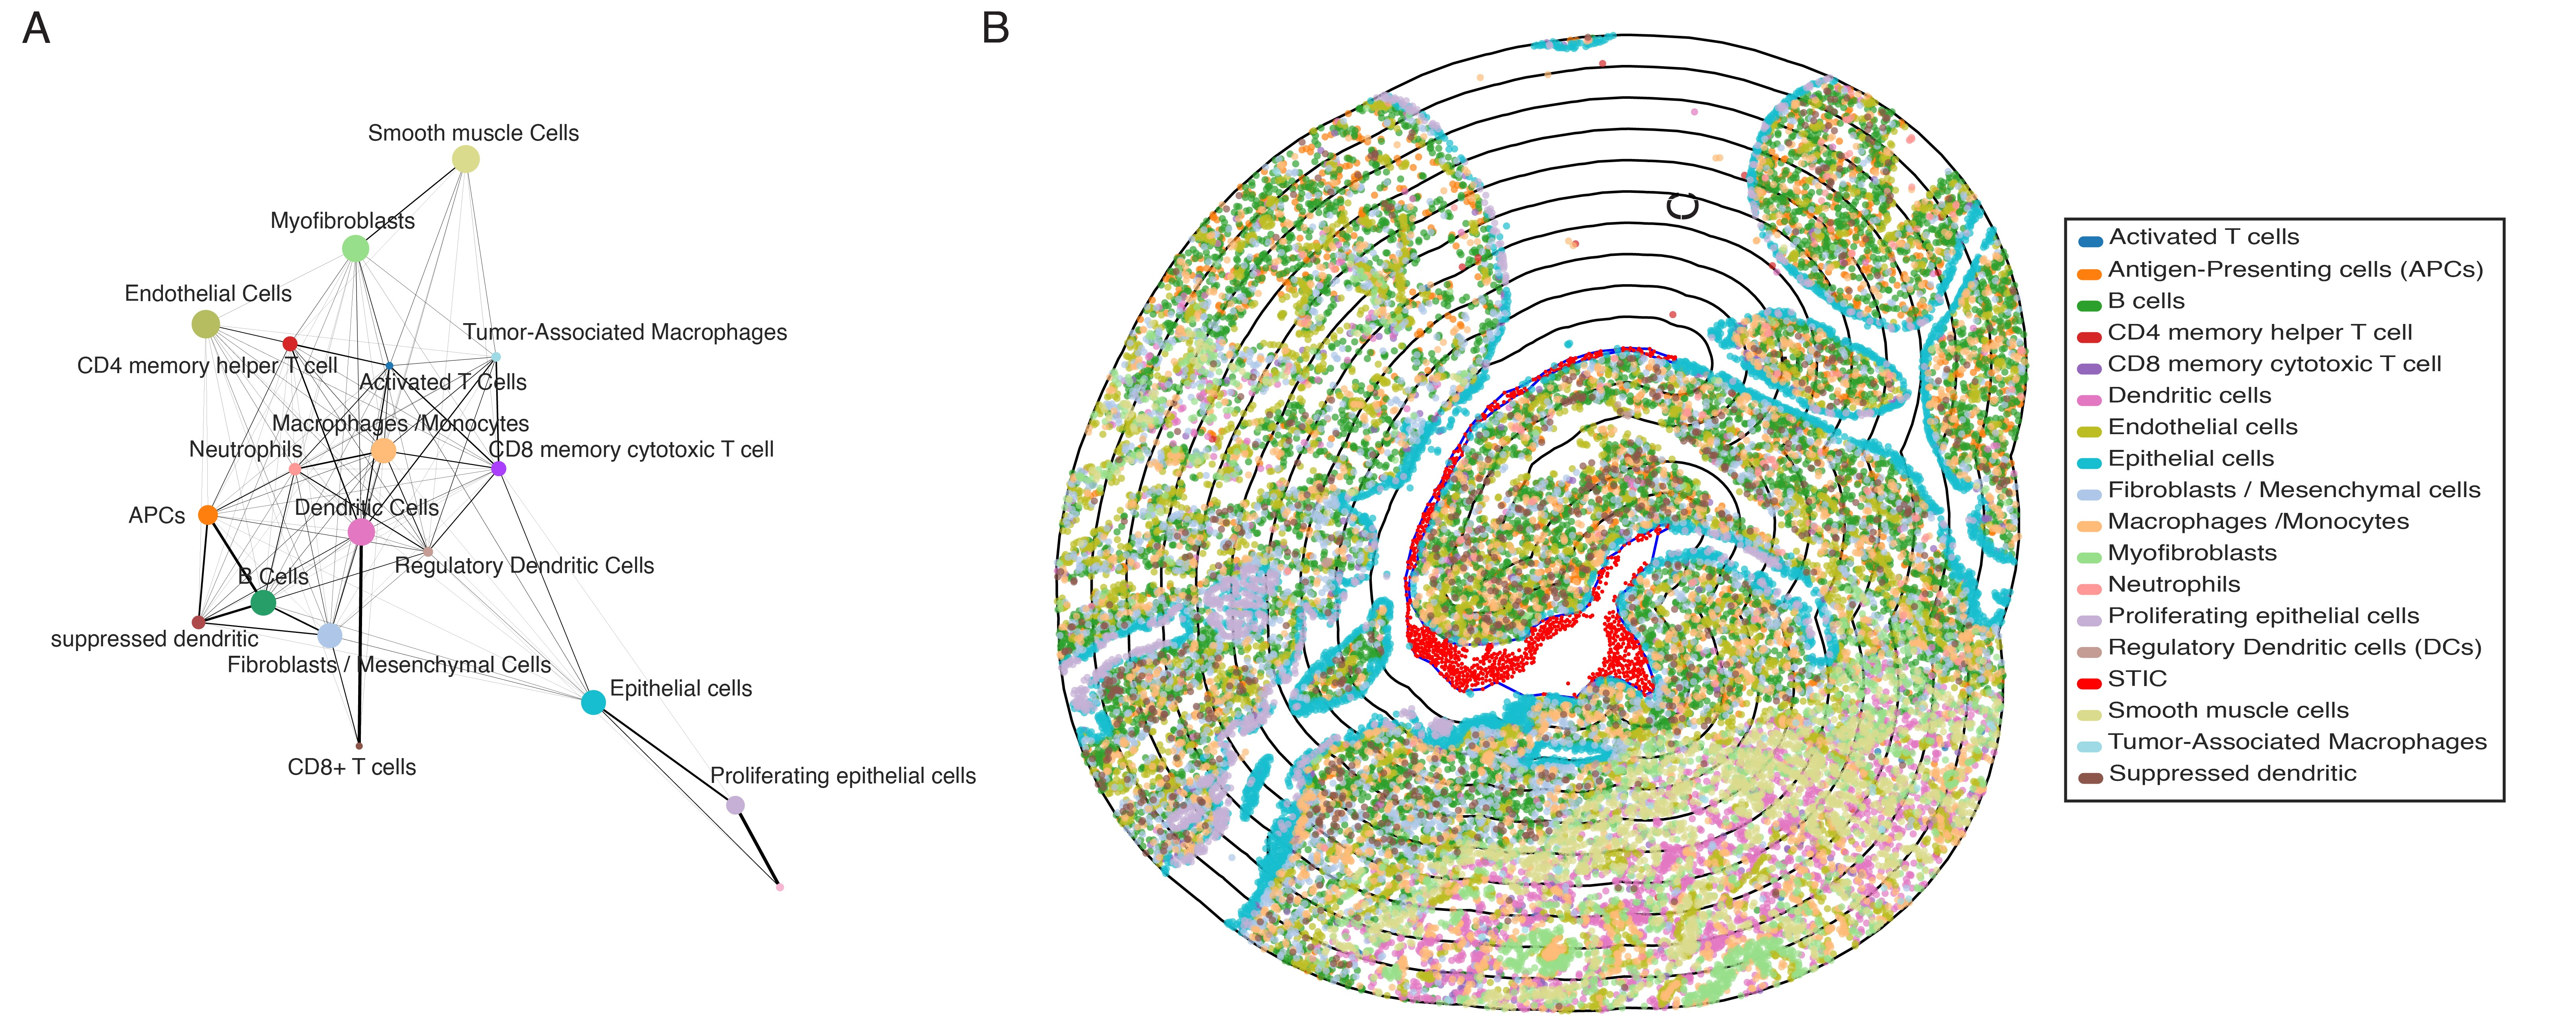
\includegraphics[width=1\textwidth,height=0.9\textheight,keepaspectratio,clip,page=1]{figures/chapter3/FigS3.jpg}
            \captionsetup{font=small}
            \caption{ \textbf{Topological and spatial proteomic mapping of proliferative active STIC microenvironment.} (a) PAGA unpruned network analysis shows cellular interactions, highlighting immunosuppressive populations near proliferative active STIC. (b) Active STIC region was masked and subsequently dilated to generate 10 micron distances. At each distance, the cellular composition was assessed. Black lines in the figure indicate incremental 100 micron distance from the STIC in red.}
            \label{chapter3_figS3}
        \end{center}
    \end{figure}
    
    
    \subsection{Spatial metabolomics profiling of STIC in non-diseased human fallopian tubes}
    Existing single cell and spatial transcriptomics data analysis has shown association of fallopian tube epithelium to genes and pathways associated with metabolic regulations in various contexts\cite{Dinh2021Single,Ulrich2022Cellular,Weigert2025cell}. With this in mind, we carefully evaluated unsaturated lipid level and redox ratio of preneoplastic epithelial lesions by multimodal two-photon stimulated Raman scattering imaging (SRS) (Figures \ref{chapter3_fig5}A-C,\ref{chapter3_figS4}A and \ref{chapter3_figS5}A-C). We found that the unsaturated lipid level was reduced while the redox ratio indicated by NADH/FAD was increased in the lesion cells compared to the healthy surrounding cells (Figure \ref{chapter3_fig5}C), suggesting the lesion epithelia subjects to ROS stress and metabolic remodeling towards glycolysis\cite{Alhallak2016Optical}. Worth noting that the scattered distribution of NADH and FAD signals in lesions (Figure \ref{chapter3_fig5}C in cyan and magenta) may indicate the fragmented mitochondria with compromised metabolic function.  We further applied hyperspectral SRS imaging and lipid subtype detection\cite{Zhang2024Multi} to perform an in situ lipidomic analysis and identified that lesions represented a distinct lipid profile manifesting in upregulated ceramide/PE and PC/PE ratio (Figures \ref{chapter3_fig5}D-F and \ref{chapter3_figS4}B), aligning with a study showing the disturbed homeostasis of ceramides and phospholipids in abnormal epithelial context\cite{Gao2013Aberrant}. 
    Interestingly, Raman spectra showed distinct changes of lipid profile in different types of lesions (Figures \ref{chapter3_figS5}D-F), suggesting the lipid metabolism is highly sensitive to the lesions and different lipid profile may represent the trajectory of lesion development. Altogether, our results provide new insights into the molecular mechanisms underlying the lesions of fallopian tube epithelium.


    \begin{figure}[p]
        \begin{center}
            \includegraphics[width=1\textwidth,height=0.9\textheight,keepaspectratio,clip,page=1]{figures/chapter3/Fig5.jpg}
            \captionsetup{font=small}
            \caption{ \textbf{Multimodal SRS imaging reveals the metabolic remodeling in lesions.} (a) P53 staining shows the lesion regions. (b) SRS protein channel overlayed with second homogenization (SHG) signal for collagen to show the architecture of the same lesion region of interest (ROI) in (a). Scale bar: 200 µm.}
            \label{chapter3_fig5}
        \end{center}
    \end{figure}
    
    \begin{figure}[h!]
        \ContinuedFloat
        \captionsetup{font=small}
        \caption[]{(c) Multimodal SRS imaging shows the comparation of multiple metabolites between control and lesion ROI. Scale bar: 20 µm. (d) Hyperspectral SRS imaging and unsupervised clustering showing the distribution of metabolites across the whole ROI shown in (A) and (B). (e) Hyperspectral SRS imaging and unsupervised clustering shows the difference of metabolic profiles between control and lesion ROI. Red arrows points to the typic Raman lipid peaks at 2850 cm-1 and 2880 cm-1. (f) The ratio images of ceramide/PE and PC/PE highlight the lipid subtype modulation between control and lesion ROI.}
    \end{figure}

    \begin{figure}[p]
        \begin{center}
            \includegraphics[width=1\textwidth,height=0.9\textheight,keepaspectratio,clip,page=1]{figures/chapter3/FigS4.jpg}
            \captionsetup{font=small}
            \caption{ \textbf{STIC lipid subtype characterization.} (a) Multimodal SRS imaging displays the protein, lipid, unsaturated/saturated lipid, NADH, FAD and radiometric images of unsaturated/saturated lipids, NADH/FAD of the ROI shown in (Figure 1A). Scale bar: 200 µm. (b) SRS hyperspectra based lipid subtype detection showing the difference in lipid subtype levels between control and lesion ROI. }
            \label{chapter3_figS4}
        \end{center}
    \end{figure}
    

    \begin{figure}[p]
        \begin{center}
            \includegraphics[width=1\textwidth,height=0.9\textheight,keepaspectratio,clip,page=1]{figures/chapter3/FigS5.jpg}
            \captionsetup{font=small}
            \caption{\textbf{Spatial metabolomic profiling on additional targeted ovarian cancer lesions.} (a-c) Multimodal and hyperspectral SRS imaging displays the metabolic states changes in multiple lesion tissues. Scale bar: 200 µm. (d-e) SRS hyperspectra from different lesion tissues underscore the consistent lipid metabolic remodeling. Red arrows points to the typic Raman lipid peaks at 2850 cm-1 and 2880 cm-1.}
            \label{chapter3_figS5}
        \end{center}
    \end{figure}
    
    \begin{figure}[h!]
        \ContinuedFloat
        \captionsetup{font=small}
        \caption[]{(c) Multimodal SRS imaging shows the comparation of multiple metabolites between control and lesion ROI. Scale bar: 20 µm. (d) Hyperspectral SRS imaging and unsupervised clustering showing the distribution of metabolites across the whole ROI shown in (A) and (B). (e) Hyperspectral SRS imaging and unsupervised clustering shows the difference of metabolic profiles between control and lesion ROI. Red arrows points to the typic Raman lipid peaks at 2850 cm-1 and 2880 cm-1. (f) The ratio images of ceramide/PE and PC/PE highlight the lipid subtype modulation between control and lesion ROI.}
    \end{figure}
    
    \subsection{Spatial transcriptomic profiling of STIC in nondiseased human fallopian tubes}
    Using the CODA IHC-based deep learning method, we profiled STIC with spatial transcriptomics (Fig. \ref{chapter3_fig6}A). STIC location was processed using Visium Cytassist for whole transcriptome profiling. Curation of the spatial spots identified STIC epithelial spots in red and non-STIC epithelial spots in green (Fig. \ref{chapter3_fig6}B).
    Differential gene expressions of the proliferative active STIC against normal adjacent epithelium were obtained and shown in volcano plot (Fig. \ref{chapter3_fig6}C). The upregulated genes in STIC, including KIF1A, TUBB2B, DLGAP5, BUB1, KIF2C, CDCA8, CDC20, CCNF, CCNB1, and PBK, suggest dysregulated cell cycle progression, mitotic spindle function, and chromosomal instability, which are seen in high-grade serous ovarian cancer\cite{Zhang2021Knockdown,Schneider2017AURKA,Hosea2024two,Chong2018Deregulation,Moura2014High,Yang2022CCNB1,Chen2025Tumor,Ikeda2016T,Comisso2017OCT4,Tang2021Pan,Fu2020Computational}.  Immune-related genes like ULBP3 and BTNL2 may contribute to immune evasion, while JUN and NOX4 could promote survival and oxidative stress responses\cite{Sun2025NOX4,Du2022Cancer,McGilvray2010ULBP2,Wang1999Microtubule}. The presence of HNF4A, TFAP2A, and ADAM12 further supports a link to ovarian carcinogenesis through transcriptional deregulation, cellular differentiation, and extracellular matrix remodeling\cite{Mai2021Histone,Du2015Screening,Cheon2015ADAM12}. These findings reinforce STIC’s role as a precursor to high-grade serous carcinoma, with key drivers of malignancy already active\cite{Schweizer2025Spatial}. Comparative analysis revealed significant upregulation of genes such as GPX2 (implicated in oxidative stress response) and HIST1H1D (a chromatin regulator) in STICs (Fig. \ref{chapter3_fig6}D), mirroring patterns observed in advanced ovarian tumors\cite{Wang2019GPX2,Parssinen2008Identification}.
    Pathway analysis using the Hallmarks gene sets\cite{Liberzon2015Molecular}, and the suppressed and activated pathways were computed (Fig. \ref{chapter3_fig6}E-F). Hallmark pathway analysis revealed enrichment of several cancer-associated pathways in STICs, including spermatogenesis, G2M checkpoint, KRAS signaling, E2F targets, oxidative phosphorylation, and TNF$\alpha$ signaling via NFkB\cite{Chang2025Integrated,Rohozinski2009Spermatogenesis,Ouyang2009Genistein,Hendrikse2023potential,Zhan2016E2F1,Nayak2018Oxidative,Maccio2012Inflammation, Harrington2019NF}. These activated pathways are consistent with clinical observations of early oncogenic signaling in STIC lesions that precede invasive high-grade serous carcinoma development\cite{Weigert2025cell} 116. Gene set enrichment analysis profiles confirmed significant enrichment of proliferation-associated pathways and G2M checkpoint genes (Fig. \ref{chapter3_fig6}G), showing dysregulated cell cycle characteristics of both STICs and invasive ovarian cancers.
    To investigate chromosomal instability in proliferative active STIC, copy number analysis (CNA) was inferred from the spatial transcriptomics data (Fig. \ref{chapter3_fig6}H-I, Fig. \ref{chapter3_figS6}F), which revealed gains in chr6p22, chr6p21, chr1p32, and chr16p13, and losses in chr17p13, chr9q33, chr9q34, chr22q11, chr22q12, and chr22q13. These results align with clinical genomic studies showing that copy number alterations and genomic instability are early events in STIC lesions\cite{Wu2019Genomic,Chang2025Integrated,Devlin1996High,Zhakula2024Patterns}. Chromosomal 6 gains and chromosomal 22 depletions were spatially located on the STIC (Fig. \ref{chapter3_fig6}K). Notably, gains in chr6p, which harbors immune-related genes, have been linked to immune evasion and tumor progression in ovarian cancer, while losses in chr17p13, encompassing TP53 and are associated with impaired DNA damage response and genomic instability \cite{Zhakula2024Patterns}. These alterations may collectively contribute to early malignant transformation and aggressive phenotypes in STIC lesions. 
    To further explore chromosomal alterations, we also applied inferCNV (Fig. \ref{chapter3_figS6}F) and identified chromosomal gains in chromosomes 1, 6, 8, 16, and 19. Chromosomal losses were detected in chromosomes 4, 9, 13, 15, 17, 18, and 22.  Comparison to a large cohort study of 47 patients with proliferative active STICs\cite{Chang2025Integrated}, which showed chromosomal gains in chromosomes 1, 2, 3, 6, 7, 8, 10, 12, 16, 19, and 20; and chromosomal depletions in chromosomes 4, 5, 6, 7, 8, 9, 11, 13, 15, 16, 17, and 22. Similarly, genes altered in these regions include TP53 (chr17p13), MYC (chr8q24.21), CCNE1 (chr19q12), CDKN2A/CDKN2B (chr9p21), BRCA1 (chr17q21), and NF2/TIMP3 (chr22q12-13).These chromosomal targets highlight pathways associated with cell cycle regulation, DNA repair, and immune modulation. Conversely, the large patient cohort study also reported unique gains in chr2, chr3, chr7, chr10, chr12, and chr20, and unique losses in chr5, chr7, chr8, and chr11, not observed in our nondiseased, average-risk donor cohort analysis. These regions encompass genes such as PIK3CA/MECOM (chr3q26), ETV6/FOXM1 (chr12p13), and APC (chr5q22), which are involved in PI3K signaling, transcriptional regulation, and tumor suppressor pathways. 

    \begin{figure}[p]
        \begin{center}
            \includegraphics[width=1\textwidth,height=0.85\textheight,keepaspectratio,clip,page=1]{figures/chapter3/Fig6.jpg}
            \captionsetup{font=small}
            \caption{\textbf{ Spatial transcriptomic profiling reveals molecular alterations in STIC lesions.} (a) Selection of STIC regions for spatial transcriptomics profiling, validated by p53 and Ki67 IHC. (b) Identification of STIC and non-STIC epithelial regions within the Visium spatial transcriptomics platform. (c) Heatmap of differentially expressed genes in STIC lesions, highlighting key upregulated and downregulated targets (adjusted p-value < 0.05).(d) Oncogene expression patterns (e.g., GPAT2, HIST1H1D) specific to STIC regions. }
            \label{chapter3_fig6}
        \end{center}
    \end{figure}
    
    \begin{figure}[h!]
        \ContinuedFloat
        \captionsetup{font=small}
        \caption[]{(e-f) Dot plots of enriched gene signatures in STIC, including KRAS signaling, oxidative phosphorylation, and epithelial-mesenchymal transition. (g) Chromosomal ploidy analysis showing copy number variations in STIC, with focal changes on chromosomes 6 and 22.}
    \end{figure}

    \begin{figure}[p]
        \begin{center}
            \includegraphics[width=1\textwidth,height=0.55\textheight,keepaspectratio,clip,page=1]{figures/chapter3/FigS6.jpg}
            \captionsetup{font=small}
            \caption{ \textbf{Spatial expression of ovarian cancer related genes, and pathway analysis.} (a)  TMNT1 and CDC20 gene expression patterns specific to STIC regions. (b) Sets of classical and basal gene expression did not show any STIC specific expression.(c) Dot plots showing significantly enriched terms from Gene Ontology Biological Process. (d) Dot plots showing significantly enriched terms from Gene Ontology Cellular Components. (e) Dot plots showing significantly enriched terms from Hallmark gene set. Dot size represents gene count, color intensity indicates adjusted p-value, and x-axis shows normalized enrichment score (NES). Terms are ordered by statistical significance. (f) Inferred CNA using inferCNV for two Visium sections of the same proliferative active STIC. Chromosomal gains are shown in red, and chromosomal depletions are shown in blue, with respect to reference adjacent healthy epithelial cells (top rows).}
            \label{chapter3_figS6}
        \end{center}
    \end{figure}

    \clearpage 
    
    \section{Methods}
    \subsection{Tissue acquisition and processing of entire human fallopian tubes}
    After resection of non-diseased human fallopian tubes from a donor network (nPOD). Specimens were processed into FFPE tissue blocks. Then, exhaustively serial sectioned at 4 microns and H\&E stained (one every two sections). Unstained slides were stored in -20$\degree$C, under optimal humidity and vacuum conditions. 
    H\&E-stained slides were scanned at 20x resolution (~0.5 micron/pixel) using a Hamamatsu Nanozoomer S210. NDPI files were converted to tiff images (1 micron/pixel) and aligned into a 3D volume. StarDist method was employed to perform nuclear segmentation of all H\&E-stained whole slide in entire fallopian tube samples. 
    
    \subsection{CODA microanatomical labelling of WSI of human fallopian tubes}
    To label the microanatomical components of the human fallopian tube, we developed two CODA semantic segmentation models\cite{Kiemen2022CODA,Matos2025CODAvision}. One model labelled the surrounding epithelium microenvironment, including blood vessels, nerves, vasculature, mesothelium, rete ovarii in all WSI (Fig. \ref{chapter3_figS1}, middle top panel). The second model was designed to automatically annotate the secretory and ciliated epithelial cells (Fig. \ref{chapter3_figS1}, middle bottom panel). Models were combined to fully segmented all whole slide images in the human fallopian tubes (Fig. \ref{chapter3_figS1}, right panel). InterpolAI was used to generate missing images to restore microanatomical connectivity \cite{SaurabhInterpolAI}.
    
    \subsection{Alignment of 2D WSI into 3D maps of entire human fallopian tubes}
    Combination of global rigid and local elastic image registrations allowed reconstruction of microanatomical structures of human fallopian tubes into 3D volume\cite{Kiemen2022CODA,Forjaz2025PIVOT}. Alignment was applied to images subtyping the epithelium and to images labelling the fallopian tube microenvironment. 
    
    \subsection{Nuclear segmentation in H\&E-stained images}
    To extract all 2.19 billion nuclear segmentations from 2,452 H\&E-stained images, we used an adapted version of the StarDist pipeline for 3D histological slides (Fig. \ref{chapter3_figS1}C)\cite{Forjaz2025Integration,Schmidt2018Cell}. StarDist 40x resolution H\&E segmentation pretrained model was finetuned to 20x resolution NDPI file format images\cite{Schmidt2018Cell}. To finetune the model, we annotated 25 H\&E stained tiles with 256x256 dimensions for training. Training was optimized finetuning hyperparameters such as learning rate, training epochs, data augmentation. To maximize the heterogeneity of the testing tiles, we se4lected tiles from regions of the human fallopian tubes and across different specimens.
    
    \subsection{Registration of 2D nuclear segmentation into 3D cellular volume}
    Similarly to the semantic segmentation step, segmented cell nuclei was registered into a 3D aligned volume, using CODA point cloud base registration method, which allowed the same alignment of the cell nuclei centroids accordingly with the tissue labelling registration\cite{Forjaz2025Integration}. Each cell on the 3D volume contained a unique cell ID, which allowed to link each cell to its respective morphological features. 
    
    \subsection{Measurement of bulk cellular and volumetric quantifications}
    With the generated 3D tissue and cellular volumes, bulk quantifications can be extracted. To obtain volumetric data from each respective label, all voxels of each respective tissue component are summed and, subsequently, adjusted according to its respective voxel size. Bulk cellular information of each microanatomical label can be extracted in silico by combination of 3D tissue labelled volume with its respective label locations in the 3D cellular volume.
    
    \subsection{3D cellular and volumetric variability within human fallopian tube epithelium}
    To quantify the variability in cellular and volumetric content within each human fallopian tube, a virtual path was generated along the epithelium. Along this virtual epithelium path, cross sections perpendicular to this path were generated to simulate travelling across the human fallopian tube epithelium. Cellular and volumetric measurements were obtained for each cross section, resulting in tens of thousands of virtual cross sections along each fallopian tube.
    
    \subsection{Detection of p53 signatures, proliferative dormant and active STICs in human fallopian tubes}
    To 3D map precursors to ovarian cancer in whole human fallopian tubes, we developed a framework that integrates H\&E and IHC (p53 and Ki67) staining methods in 3D. First, we developed a deep learning method to identify positive signal locations in p53 and Ki67 IHC stained images (stained one in every 8 sections of the entire stack of images). Then we aligned the IHC images to the aligned H\&E-stained image stack. Combination of IHC stained slides and H\&E-stained slides to highlight regions with potential precursors of ovarian cancer. Generation of the lesions image stacks containing IHC and H\&E images to manually check hundreds of potential lesion locations across different specimens. Manual validation of each bounding box with pathologists and trained experts allowed the compiling of confirmed ovarian cancer precursors. Validated lesions were then used for further multi-omics profiling.
    
    \subsection{Volume distribution of ovarian cancer precursors across different samples}
    For each individual validated lesion, their volume was computed (Fig.\ref{chapter3_fig3}F, left panel). Power law was used to predict lesion growth for proliferative active and  dormant STICs, and p53 signatures combined (Fig. \ref{chapter3_fig3}F, middle panel)\cite{Power}. Using the Kolmogorov-Smirnov test, maximization of the p-value was applied to fit the measured lesion volumes\cite{Massey1951Kolmogorov}.
    
    \subsection{3D virtual SEE-FIM procedure for detection of epithelial lesions in low-risk nondiseased human fallopian tube samples}
    To virtually simulate the SEE-FIM procedure in our samples, we generated a virtual path across the human fallopian tube’s epithelium. In the fimbriated ends of the fallopian tube, longitudinal sections were generated, and on the remaining of the fallopian tube transverse cross sections were computed. For each fallopian tube sample, equally distanced slides were generated ranging from 1 up to 11,000 sections along the epithelium’s center path (Fig. \ref{chapter3_fig3}G, and Fig. \ref{chapter3_figS2}D). Simulations of the distinct virtual section ranges were computed for each fallopian tube (Fig. \ref{chapter3_figS2}E) and, for each combination of sections simulated, the number of lesions was assessed. The same was computed to the respective percentage of the fallopian tube sectioned (Fig. \ref{chapter3_fig3}H).
    
    \subsection{Spatial proteomics on region of interest to map STIC immune landscape}
    To deeply profile the proteomic landscape involved in STIC progression, we applied CODEX spatial proteomics using 25 marker antibody panel targeting epithelial, immune, and stromal populations (Fig. \ref{chapter3_fig4}A). WSI cyclic immunofluorescence was conducted to ensure spatial comparison of STIC to non-lesional epithelia. DAPI nuclear channel was segmented and subsequent dilation of the nuclear area ensured cells were isolated and boundaries of each were accurately delimited (Fig. \ref{chapter3_fig4}B) \cite{Schmidt2018Cell}. For each segmented cell, protein expression intensities were quantified. Marker intensities were normalized to minimize the effects of inter-cell variability. UMAP was applied to visualize multidimensional protein expression profiles and identify distinct cellular clusters (Fig. \ref{chapter3_fig4}C) \cite{Squidpy,Wolf2018SCANPY,Virshup2021anndata,Krzywinski2009Circos,Hunter2007Matplotlib,Waskom2021seaborn,McInnes2020UMAP,Shimoyama2022pyCirclize,pandas2024pandas,Harris2020Array,Pedregosa2011Scikit}. Clusters were annotated based on canonical marker expressions to distinguish epithelial, stromal, and immune cell populations (Fig. \ref{chapter3_fig4}D-F). 
    Spatial mapping was then performed to measure the distribution of cell types across the STIC and adjacent epithelial regions (Fig. \ref{chapter3_fig4}G-I). To investigate the cell-to-cell interaction between the cell phenotypes, we applied a PAGA (Partition-based Graph Abstraction)\cite{Wolf2019PAGA}. Using PAGA, we inferred proximity and connectivity between cell phenotypes (Fig. \ref{chapter3_fig4}G, \ref{chapter3_figS3}A). 
    To compute the variance in cellular composition relative to STIC proximity, we performed a spatial dilation of the STIC mask and measured the cellular composition at different distances (Fig. \ref{chapter3_figS3}B). Cell type composition was calculated every 10 µm distances and extended up to 500 µm from STIC region (Fig. \ref{chapter3_fig4}H). Quantification of the differential cellular enrichment was quantified by comparing regions within 100 µm to this STIC to regions distancing 400 and 500 µm from the STIC (Fig. \ref{chapter3_fig4}I).
    
    \subsection{Two-photon stimulated Raman scattering to map metabolomic signature in STIC}
    Pathologist-validated lesions within 3D spatial maps of fallopian tubes were selected for spatial metabolomics analysis of the ovarian cancer precursors (Fig. \ref{chapter3_fig5}A). High-resolution multimodal two-photon stimulated Raman scattering (SRS) imaging was used to quantify metabolic signatures across lesions\cite{Zhang2024Multi}. Multimodal SRS imaging targeting lesions and control normal adjacent epithelial regions of interest (ROIs) allowed to capture spatial distributions of proteins, saturated and unsaturated lipids, total lipids, NADH, and FAD (Fig. \ref{chapter3_fig5}B-C). Intensity-normalized images were concatenated into feature vectors and analyzed by principal-component analysis followed by k-means clustering (Fig. \ref{chapter3_fig5}D-E)\cite{Ikotun2023K}.
    
    \subsection{Spatial transcriptomic profiling of low-risk non-diseased STIC }
    3D mapped regions containing STIC were selected and used to guide placement of the Visium CytAssist capture area (6.5 x 6.5 mm$^2$). Tissue sections were processed using the 10x Genomics Visium CytAssist FFPE protocol. After deparaffinization and epitope retrieval, hybridization with the Human Transcriptome Probe Set v2.0. Probe release was conducted via CytAssist, followed by library preparation and sequencing (~250 million reads/sample) on an Illumina NovaSeq 6000\cite{Johnson2025Human,Bell2024PanIN}.
    Differential gene expression analysis between STIC and normal regions was performed using Seurat v5 \cite{Hao2024Dictionary}. Genes with adjusted p-value <0.05 and log2 fold change >0.25 were considered significant (Fig. \ref{chapter3_fig6}C, \ref{chapter3_figS6}A-B). Significantly altered genes were subjected to Gene Ontology (GO) analysis (Fig.  \ref{chapter3_fig6}E) and Hallmark pathway enrichment using GSEA (Fig. \ref{chapter3_fig6}F–G, \ref{chapter3_figS6}C-E)\cite{Subramanian2005Gene,Ashburner2000Gene,Aleksander2023Gene}. Enrichment scores were visualized using dot plots and ranked enrichment plots. Copy number alterations were inferred from transcriptomic data using inferCNA and inferCNF, comparing STIC spots to adjacent normal epithelial reference regions\cite{Patel2014Single,Timothyinfercnv}. Alterations were visualized as heatmaps and chromosome-specific dot plots (Fig.  \ref{chapter3_fig6}H–I). Spatial distribution of chromosomal alterations was mapped across tissue sections (Fig. \ref{chapter3_fig6}J–K, Fig. \ref{chapter3_figS6}F).
    
    \subsection{Statistical considerations}
    All significance tests were performed using the Wilcoxon rank sum test. To compare metrics within and between cohorts, median, mean, standard deviation, and interquartile range were determined. Relative error was defined as [measured value – expected value] / expected value. No other statistical calculations were performed in this work.

    \clearpage
    \section{Supplemental Tables}
    
    \begin{table}[htbp]
        \centering
        \footnotesize
        \renewcommand{\arraystretch}{1.2}
        \caption{Number of sections, dimensions, total volume, and cell count for pre-menopausal and post-menopausal donor samples.}
        \label{chapter3_table_S1}
        \begin{tabularx}{\textwidth}{l l c c c c c c}
            \toprule
            \textbf{Group} & \textbf{Donor} & \textbf{Total} & \textbf{Width} & \textbf{Length} & \textbf{Depth} & \textbf{Volume} & \textbf{Total Cells} \\
            & & \textbf{Sections} & \textbf{(mm)} & \textbf{(mm)} & \textbf{(mm)} & \textbf{(cm³)} & \textbf{(Million)} \\
            \midrule
            \makecell[l]{\textbf{Post-}\\\textbf{menopausal}} & Donor 1 & 601 & 23.4 & 17.6 & 3.0 & 0.31 & 178.3 \\
            & Donor 2 & 627 & 32.8 & 24.4 & 3.1 & 0.78 & 425.9 \\
            & Donor 3 & 999 & 28.3 & 20.8 & 5.0 & 0.86 & 552.5 \\
            \makecell[l]{\textbf{Pre-}\\\textbf{menopausal}} & Donor 4 & 1305 & 21.5 & 19.4 & 6.5 & 0.75 & 509.0 \\
            & Donor 5 & 1373 & 15.5 & 32.1 & 6.9 & 0.70 & 525.8 \\
            \bottomrule
        \end{tabularx}
    \end{table}
    
    \begin{table}[htbp]
        \centering
        \renewcommand{\arraystretch}{1.2}
        \caption{Number of STIC lesions in pre-menopausal and post-menopausal donor samples.}
        \label{chapter3_table_S2}
        \begin{tabularx}{\textwidth}{l l X X X X X}
            \toprule
            \multicolumn{7}{c}{\textbf{Precancerous lesions (Proliferative active and dormant STICs)}} \\
            \midrule
            \textbf{Group} & \textbf{Donor} & \textbf{Total} & \textbf{Mean} & \textbf{Median} & \textbf{Min} & \textbf{Max} \\
            \midrule
            Pre-menopausal & Donor 1 & 0 & 8.5 & 8.5 & 0 & 17 \\
            & Donor 2 & 17 &  &  &  &  \\
            Post-menopausal & Donor 3 & 35 & 27.33 & 35 & 5 & 42 \\
            & Donor 4 & 42 &  &  &  &  \\
            & Donor 5 & 5 &  &  &  &  \\
            \bottomrule
        \end{tabularx}
    \end{table}
    
    \begin{table}[htbp]
        \centering
        \renewcommand{\arraystretch}{1.2}
        \caption{Proliferative Active STIC lesions identified in pre-menopausal and post-menopausal donor samples.}
        \label{chapter3_table_S3}
        \begin{tabularx}{\textwidth}{l l X X X X X}
            \toprule
            \multicolumn{7}{c}{\textbf{Proliferative active STICs}} \\
            \midrule
            \textbf{Group} & \textbf{Donor} & \textbf{Total} & \textbf{Mean} & \textbf{Median} & \textbf{Min} & \textbf{Max} \\
            \midrule
            Pre-menopausal & Donor 1 & 0 & 0 & 0 & 0 & 0 \\
            & Donor 2 & 0 &  &  &  &  \\
            Post-menopausal & Donor 3 & 8 & 4.33 & 5 & 0 & 8 \\
            & Donor 4 & 5 &  &  &  &  \\
            & Donor 5 & 0 &  &  &  &  \\
            \bottomrule
        \end{tabularx}
    \end{table}
    
    \begin{table}[htbp]
        \centering
        \renewcommand{\arraystretch}{1.2}
        \caption{Proliferative Dormant STIC lesions identified in pre-menopausal and post-menopausal donor samples.}
        \label{chapter3_table_S4}
        \begin{tabularx}{\textwidth}{l l X X X X X}
            \toprule
            \multicolumn{7}{c}{\textbf{Proliferative dormant STICs}} \\
            \midrule
            \textbf{Group} & \textbf{Donor} & \textbf{Total} & \textbf{Mean} & \textbf{Median} & \textbf{Min} & \textbf{Max} \\
            \midrule
            Pre-menopausal & Donor 1 & 0 & 8.5 & 8.5 & 0 & 17 \\
            & Donor 2 & 17 &  &  &  &  \\
            Post-menopausal & Donor 3 & 27 & 23.00 & 27 & 5 & 37 \\
            & Donor 4 & 37 &  &  &  &  \\
            & Donor 5 & 5 &  &  &  &  \\
            \bottomrule
        \end{tabularx}
    \end{table}
    
    
    \begin{table}[htbp]
        \centering
        \renewcommand{\arraystretch}{1.2}
        \caption{p53 Signatures identified in pre-menopausal and post-menopausal donor samples.}
        \label{chapter3_table_S5}
        \begin{tabular*}{\textwidth}{@{\extracolsep{\fill}}l l c c c c c}
            \toprule
            \multicolumn{7}{c}{\textbf{p53 Signatures}} \\
            \midrule
            \textbf{Group} & \textbf{Donor} & \textbf{Total} & \textbf{Mean} & \textbf{Median} & \textbf{Min} & \textbf{Max} \\
            \midrule
            Pre-menopausal & Donor 1 & 1 & 3 & 3 & 1 & 5 \\
            & Donor 2 & 5 &  &  &  &  \\
            Post-menopausal & Donor 3 & 1 & 1.67 & 1 & 0 & 4 \\
            & Donor 4 & 4 &  &  &  &  \\
            & Donor 5 & 0 &  &  &  &  \\
            \bottomrule
        \end{tabular*}
    \end{table}
    
    \begin{table}[htbp]
        \centering
        \renewcommand{\arraystretch}{1.2}
        \caption{Statistical prevalence of ovarian cancer precursor lesions in whole human Fallopian tube cohorts.}
        \label{chapter3_table_S6}
        \begin{tabular*}{\textwidth}{@{\extracolsep{\fill}}l c c c c}
            \toprule
            \textbf{Group} & \makecell{\textbf{\# Patients}} & \makecell{\textbf{Proliferative}\\\textbf{Active STIC}\\\textbf{Prevalence}} & \makecell{\textbf{Proliferative}\\\textbf{Dormant STIC}\\\textbf{Prevalence}} & \makecell{\textbf{p53 Signature}\\\textbf{Prevalence}} \\
            \midrule
            Pre-menopausal & 2 & 0\% (0/2) & 50\% (1/2) & 50\% (1/2) \\
            Post-menopausal & 3 & 66.67\% (2/3) & 100\% (3/3) & 66.67\% (2/3) \\
            Combined & 5 & 40\% (2/5) & 80\% (4/5) & 60\% (3/5) \\
            \bottomrule
        \end{tabular*}
    \end{table}

    \clearpage
    
    \printbibliography[heading=subbibliography, title={References}]
\end{refsection}
\chapter{Combined assembloid modeling and 3D whole-organ mapping captures the microanatomy and function of the human fallopian tube} \label{chap:chap-4}

\begin{refsection}
    \section{Introduction}
    
    The fallopian tubes are a pair of tube-like organs in the female reproductive system. Their primary functions are to catch ovulating oocytes from the adjacent ovaries, provide an environment that supports the survival of sperm and eggs for fertilization, and transport a developing embryo from an ovary to the uterus for implantation \cite{croxatto2002a,leese2001a}. This process is achieved through peristalsis driven by the fallopian tube smooth muscle and motile cilia along the fallopian tube epithelium \cite{croxatto2002a,leese2001a}. Structural and functional abnormalities are responsible for tubal (ectopic) pregnancy, a life-threatening condition if left untreated\cite{chua2017a,shao2010a}. The fallopian tubes also connect the uterine and peritoneal cavities and serve as the anatomic structure for retrograde menstruation, a leading theory of endometriosis etiology which affects 10\% of reproductive age women\cite{zondervan2018a,shafrir2018a}. Recently, the fallopian tubes have received significant attention because of a new paradigm for the onset of high-grade serous ovarian carcinoma (HGSC), the most common subtype of ovarian cancer, which posits that HGSCs arise from precursor lesions in the fallopian tube epithelium called serous tubal intraepithelial carcinomas (STICs)\cite{labidi-galy2017a,shih2021a}. The exact physical and molecular mechanisms that govern these fallopian tube conditions remain largely unknown, in part due to the lack of appropriate preclinical models\cite{chumduri2021a,alzamil2021a}. HGSC and endometriosis do not spontaneously occur in mice as they do in humans\cite{lengyel2014a,rangarajan2004a,jones2013a,mccloskey2014a,gruemmer2006a,greaves2014a,zondervan2018a}, so researchers have turned to engineered mouse models and in vitro organoid models to study these human diseases in an environment with the highest physiological similarity\cite{alzamil2021a,howell2014a,murphy2022a}. 
    Histologically, the fallopian tube mucosa, muscularis, and serosa regions are composed of unique combinations of epithelial, stromal, and/or smooth muscle cells\cite{wheeler1982a,popescu2005a}. The extracellular matrix (ECM) of these regions varies by collagen density and the presence of basement membranes, laminin, and other ECM proteins\cite{popescu2005a}. Beyond this compositional complexity, the organ undergoes dynamic changes due to peritoneal fluid\cite{lyons2002a} and the hormones and follicular fluid that are released at various stages of the reproductive cycle \cite{lyons2002a,amso1994a,crow1994a}.
    Here, we present a novel multi-compartment assembloid of the human fallopian tube. An assembloid is a type of organoid that can coculture multiple cell types and ECMs in spatially distinct regions in three-dimensional (3D) culture, thus improving the model’s compositional accuracy compared to the in situ tissue \cite{kanton2022a,pa2022a}. The ECM and cellular composition of each compartment in our model can be adjusted to closely match the tissue composition. Our multi-compartment assembloid preserved the molecular expression patterns observed in histological fallopian tube tissue sections and produced a physiological response to menstrual cycle hormone stimulation according to previously published validation parameters for the state-of-the-art (standard) fallopian tube epithelial organoid\cite{kessler2015a,xie2018a,feng2022a}. We compared multi-compartment assembloid and human fallopian tube proteomes via global label-free proteomics. A novel functional assay evaluated the multi-compartment assembloid’s functional capacity for cilia-driven transport of oocyte-mimicking microbeads along the epithelium facing the assembloid’s lumen-like region. Fallopian tube assembloids were rigorously compared to a whole healthy human fallopian tube using CODA\cite{kiemen2022a,sneider2022a,yang2022a,xue2022a,groot2021a,kiemen2023a}, a 3D imaging approach that quantitatively maps the microanatomy of organs at cellular resolution. Here, CODA was used to label fallopian tube epithelial cells and stroma. We identified biomimetic measurements that could be obtained from a defined volume near the fimbriated end of the fallopian tube, a common location for HGSC precursor lesions\cite{labidi-galy2017a,shih2021a}, and compared assembloid and tissue values. These architectural quantifications were carefully adjusted through multi-compartment assembloid parameter modifications to iteratively converge the architecture of the assembloids toward the reference map of a healthy human fallopian tube. 
    
    \section{Results}
    
    \subsection{Multi-compartment assembloids self-organize to mimic the mucosal folds of the human fallopian tube}
    Our multi-compartment fallopian tube assembloid was designed to mimic the in situ microenvironment where epithelial cells lining the fallopian tube lumen are supported by a thin basement membrane and surrounded by a collagen-rich stromal matrix (Fig. 1A). This multi-ECM microenvironment was captured in vitro by first suspending fallopian tube epithelial cells (FTECs, 1 x 104 cells/µL) in a small (1 µL) droplet of Matrigel, a solubilized basement membrane (Fig. 1B). This first compartment, which we call the assembloid core, was embedded in a larger (10 µL total assembloid volume) second compartment, which we call the assembloid corona, composed of collagen I to resemble the tissue stroma (Fig. 1C). By adding this stroma-like ECM compartment, spatially distinct regions are formed in the 3D culture that mimic the compartmentalization of the tissue. However, since the FTECs are the only cell type incorporated in this culture, we call this version of our assembloid a monoculture assembloid. Stromal cells can be incorporated into the corona compartment, producing a coculture assembloid that further improves the similarity of the cellular and ECM composition of the assembloid to the tissue. This assembloid protocol was based on an oil-in-water droplet microtechnology recently developed to generate multi-compartment tumor organoids\cite{lee2022a}. The size of the core and corona compartments within the assembloids are extremely consistent across batches (Fig. 1D). The versatility of this approach was leveraged by adjusting the concentrations of cells and ECM in the core and corona compartments to best fit the fallopian tube architecture described above. FTECs were cultured in a growth factor reduced (GFR) Matrigel core surrounded by a 2-6 mg/mL collagen I corona. 
    The standard fallopian tube organoid model forms clusters of cells with a hollow center that resemble a cell-free lumen-like region\cite{kessler2015a,xie2018a} by suspending FTECs (~400 cells/µL) in 50 µL drops of Matrigel and supplementing these cultures with inhibitors/growth factors to encourage 3D growth (Fig. 1E). The standard fallopian tube organoid model is optimal for high throughput mutagen and drug screening in the fallopian tube epithelium (28); however, for studies involving tissue architecture, coculture of epithelial and stromal cells, or the multi-ECM microenvironment of fallopian tube tissue\cite{wheeler1982a,popescu2005a}, a more complex model is required. By introducing a multi-ECM microenvironment in the multi-compartment model, the epithelial architecture also more closely mimicked the fallopian tube’s mucosal folding (Fig. 1F). This new multi-compartment approach is more complex and lower throughput, but it reduces the ECM reagents required to establish an organoid culture from 50 µL (standard) to 10 µL (multi-compartment). The standard organoid and multi-compartment assembloid architectures were also compared to a technical control where the cell density (1 x 104 cells/µL) and medium formulation (unmodified cell culture medium) used in the multi-compartment model was plated according to the standard organoid technique (50 µL drops of Matrigel on glass) (Fig. 1G). This technical control did not form the characteristic mucosal folding architecture, demonstrating the necessity of the oil-in-water technique and spherical droplets of ECM to form the interconnected mucosal folding achieved in multi-compartment assembloids (Fig. 1H).
    Intricate epithelial organization that mimicked the tortuosity of the human fallopian tube’s mucosal folds was supported in multi-compartment assembloid cultures of many different FTEC sources, including immortalized FTECs (fig. S1A) and a mixture of FTEC cell lines (fig. S1B). Standard fallopian tube organoids are often grown from primary cell cultures (28), so primary FTECs were also cultured in the multi-compartment model, producing a similar mucosal folding architecture (fig. S1C). In the standard model, organoids grow from individual cells\cite{kessler2015a}, although not all FTECs developed into organoids (fig. S1D). Both primary (fig. S1D) and immortalized (fig. S1E) FTECs were grown in the standard model as well for direct comparisons between the multi-compartment assembloid and standard organoid architectures formed by each type of cell culture. Multiple standard organoids often stacked on top of or next to each other, causing long-range interactions between separate organoids within the same FTEC culture (fig. S1E). 
    The spontaneous assembly of FTECs in multi-compartment assembloids into the mucosal architecture was not primarily driven by cell proliferation. The architecture did not begin to assemble until after day 3, but the change in proliferation from day 3 to day 7 was not significant (Fig. 1I). Instead, the formation of these folds depended on cell re-organization and interactions with the immediate and surrounding ECM (Fig. 1J, fig. S1F). The Matrigel:Matrigel (core:corona) combination (Fig. 1J – top left panel) did not allow sufficient cell growth for the assembloid architecture to mature. In the collagen I:Matrigel assembloid (Fig. 1J – bottom left panel), cell growth was contained within the core but disorganized, and in the collagen I:collagen I assembloid (Fig. 1J – bottom right panel), epithelial cells invaded the stroma-like region. The intricate architecture resembling the fallopian tube’s lumen only formed when the matrix components were organized to resemble the fallopian tube anatomy, i.e., epithelial cells were embedded in a basement membrane (Matrigel) and surrounded by a collagen I stroma-like environment (Fig. 1J – top right panel). This Matrigel:collagen I combination confined FTECs to a central mucosal region and provided the extracellular structure necessary for organized folds to form. 
    These multi-compartment assembloids can be further customized to match the in situ microenvironment, such as by adding a third compartment containing smooth muscle cells. Here and as further demonstrated below, the dual-compartment model containing epithelial cells in the core was sufficient for the spontaneous organization of an assembloid architecture resembling the fallopian tube’s mucosal folds.

    \begin{figure}[p]
        \begin{center}
            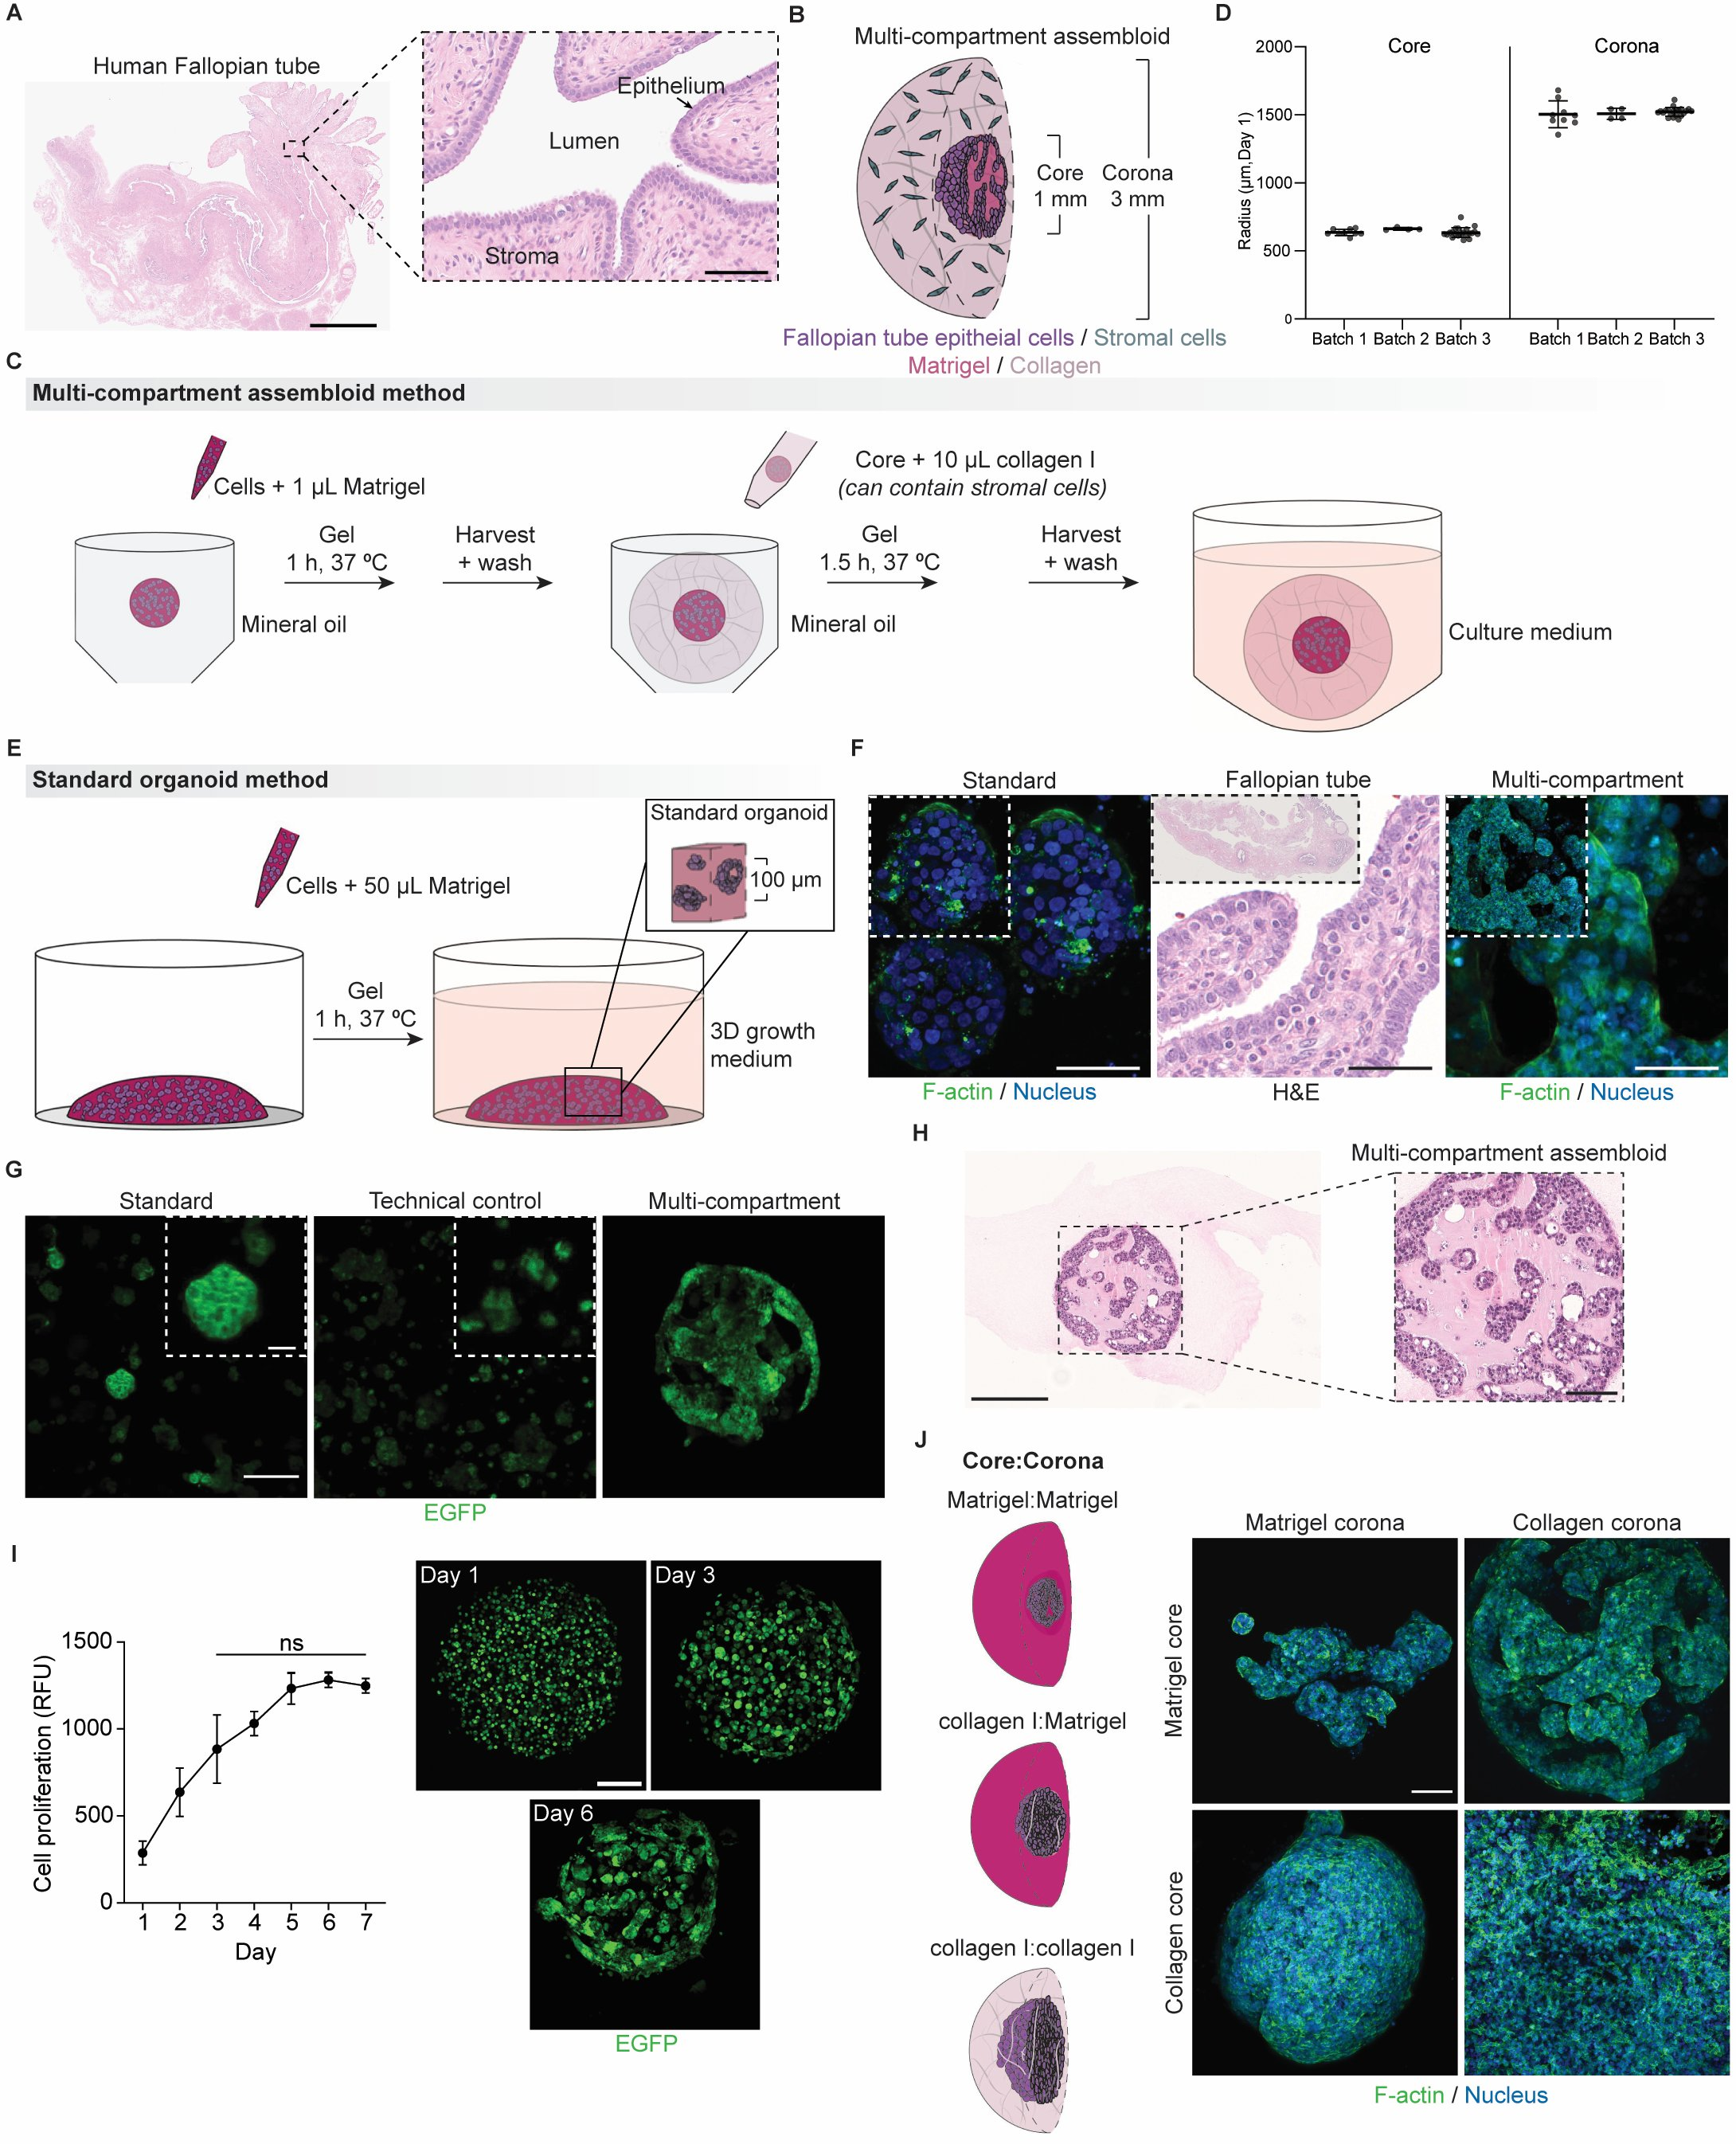
\includegraphics[width=1\textwidth,height=0.85\textheight,keepaspectratio,clip,page=1]{figures/chapter4/fig_1.jpg}
            \captionsetup{font=small}
            \caption{\textbf{Human fallopian tube assembloids.} (A) A healthy human fallopian tube tissue section. Hematoxylin and eosin (H\&E): nuclei (purple), ECM and cytoplasm (pink). Scale bar, 5 mm. Inset, 75 µm. Cartoons depicting (B) a multi-compartment fallopian tube assembloid and (C) the protocol to generate assembloids where stromal cells can be incorporated into the corona (indicated, but not shown). }
            \label{chapter4_fig1}
        \end{center}
    \end{figure}
    
    \begin{figure}[h!]
        \ContinuedFloat
        \captionsetup{font=small}
        \caption[]{(D) The radius of fallopian tube assembloid cores and whole assembloids (corona) were measured from phase-contrast images taken on day 1 of assembloid culture. The size of assembloid cores and coronas are extremely consistent within and between batches. Data are mean ± SD.  (E) Cartoon depicting the protocol to generate standard organoids and a mature standard fallopian tube organoid. (F) Side-by-side comparison of standard organoids (left), human fallopian tube tissue (middle) and multi-compartment assembloids (right). Inset is a whole organoid, fallopian tube, or assembloid. F-actin (green) and nuclear DNA (blue). Fallopian tube tissue is an H\&E stained tissue section. Scale bars, 50 µm. (G) EGFP-tagged FTECs (green) on day 6 grown in the standard organoid model (left), a technical control (middle), and the multi-compartment assembloid model (right). Scale bar, 250 µm. Inset, 50 µm. (H) H\&E image of a fallopian tube multi-compartment assembloid. Scale bar, 300 µm. Inset is the epithelial region of the assembloid. Inset scale bar, 100 µm. (I) PrestoBlue net proliferation in multi-compartment assembloids with timepoint images of EGFP-tagged multi-compartment assembloids (green). Scale bar, 250 µm. N = 3, n = 4+. Statistical test: one-way ANOVA, ns P > 0.05. Data are mean ± SEM. (J) Representative images of multi-compartment assembloids with all permutations to the assembloid ECM. F-actin (green) and nuclear DNA (blue). Scale bar, 100 µm. All organoid/assembloid images are maximum intensity projections of stacks of confocal microscopy images.}
    \end{figure}

    \begin{figure}[p]
        \begin{center}
            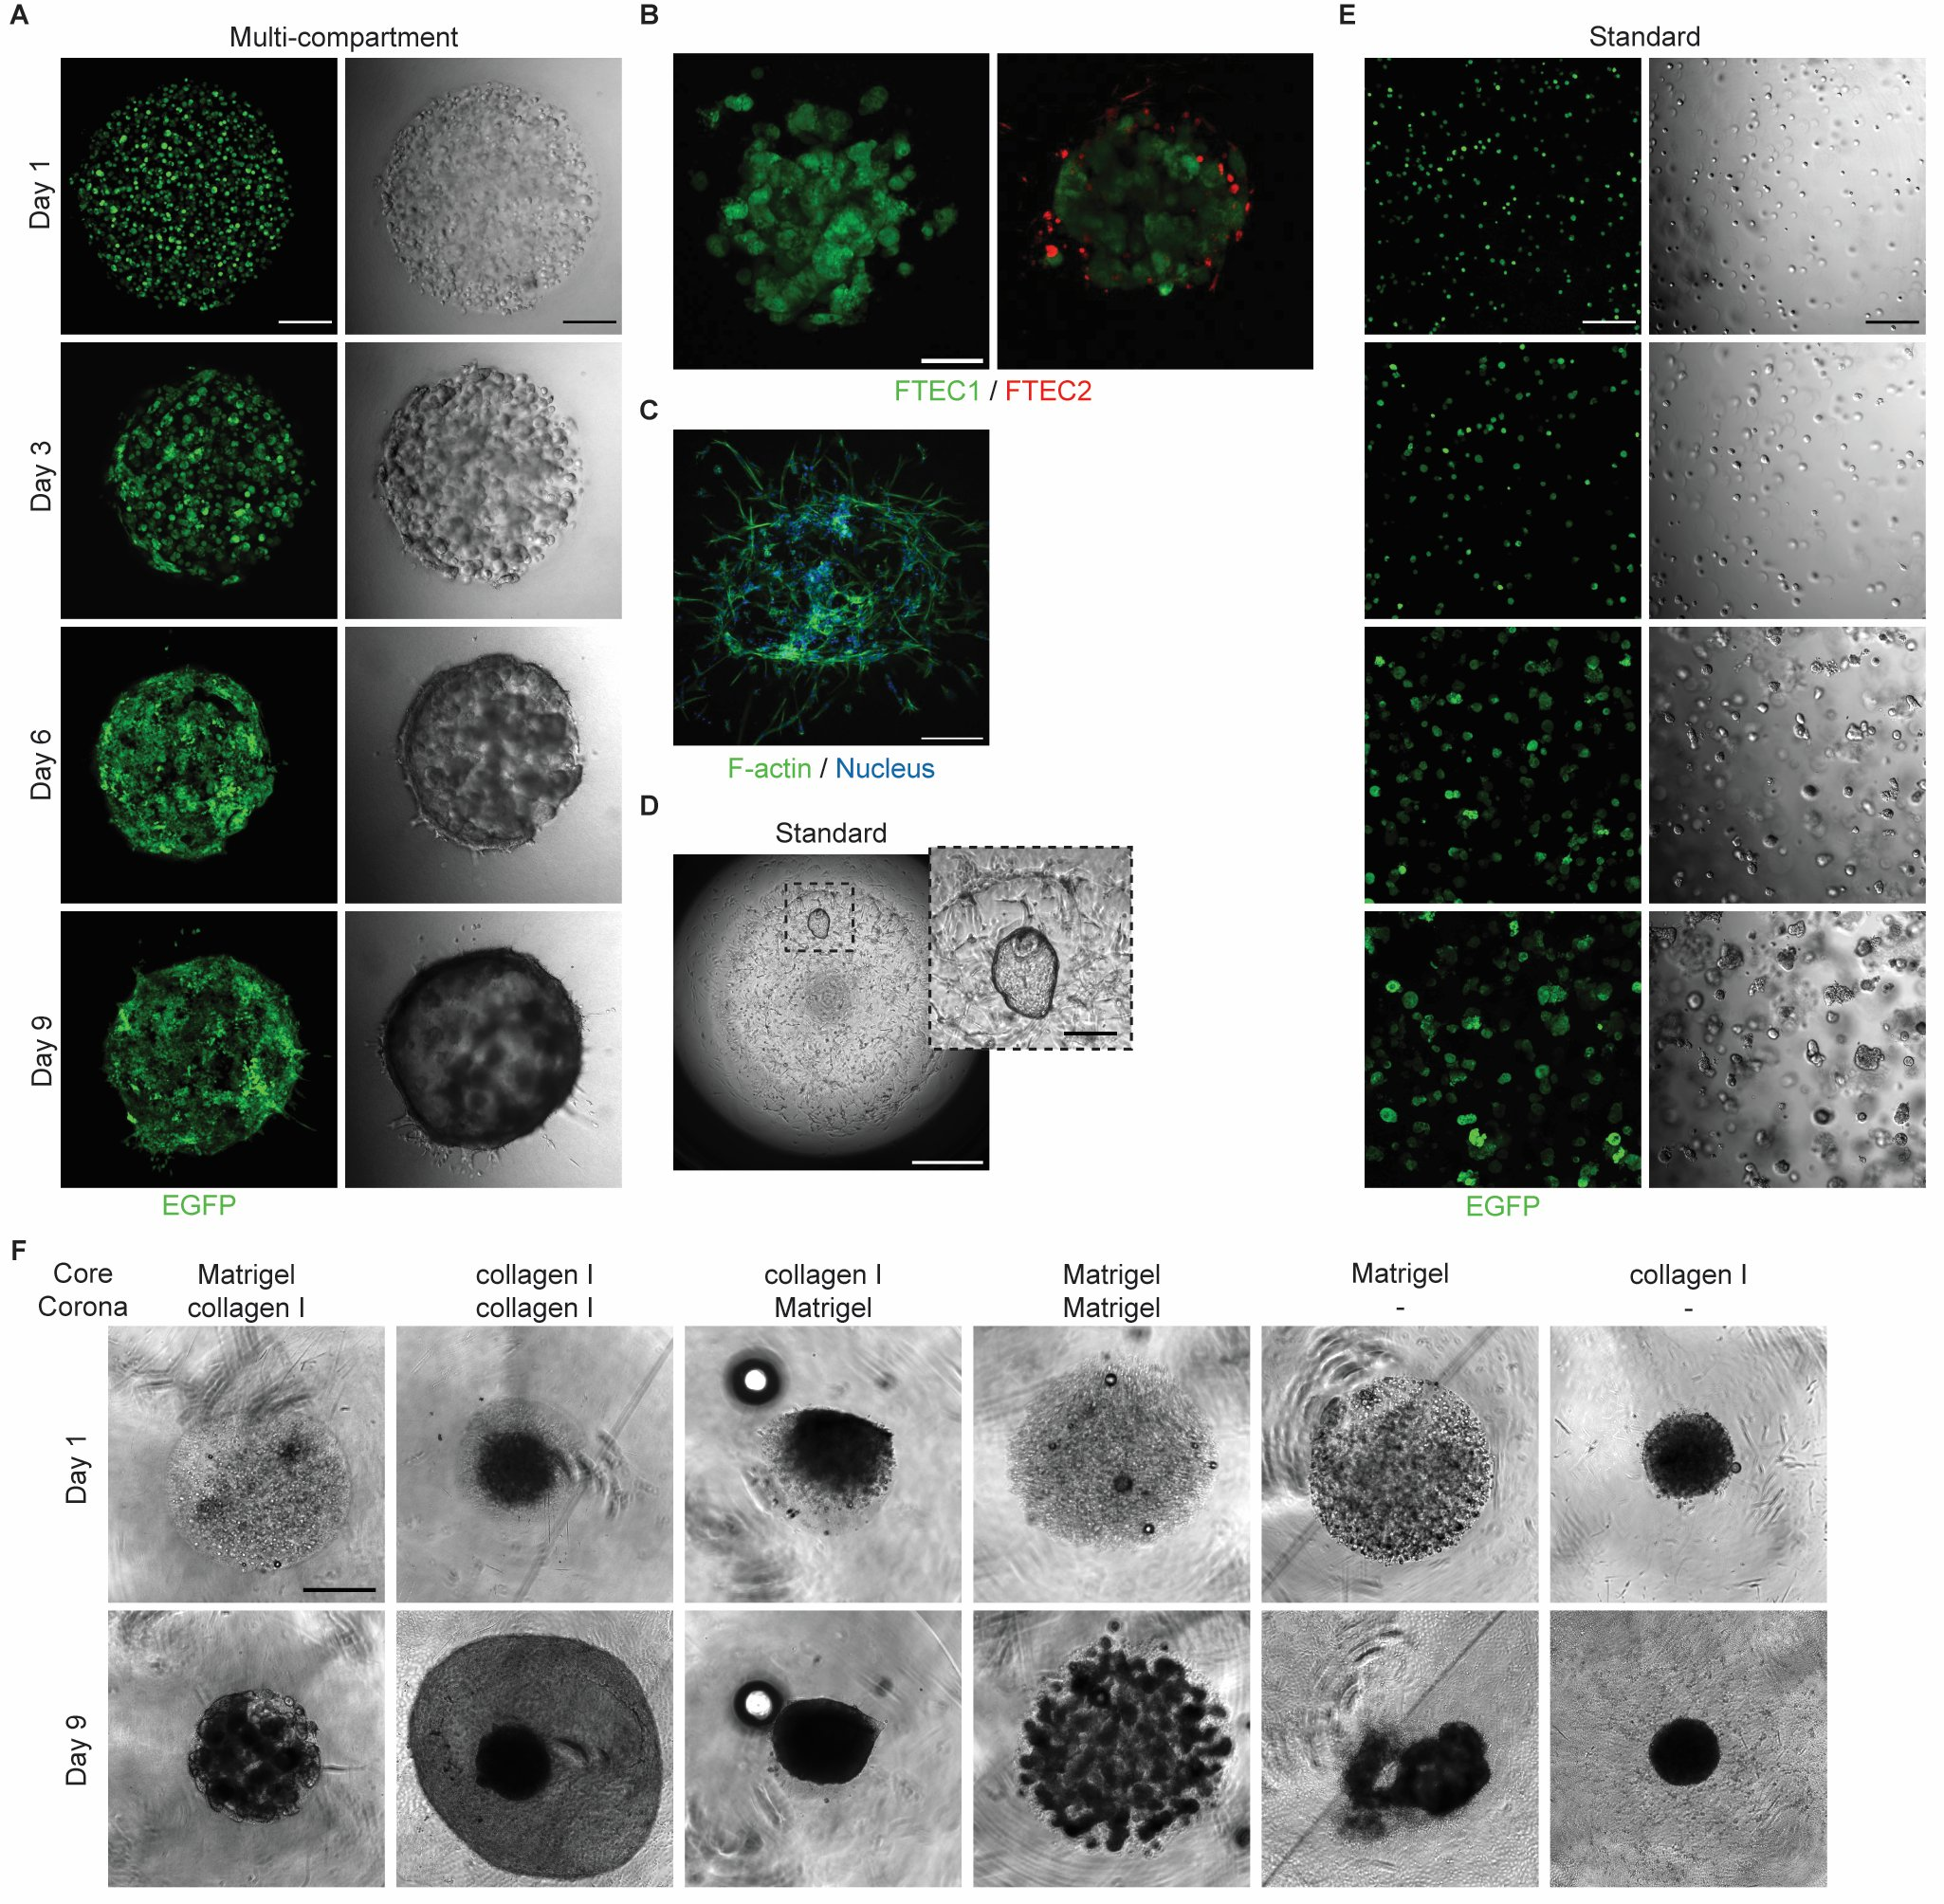
\includegraphics[width=1\textwidth,height=0.85\textheight,keepaspectratio,clip,page=1]{figures/chapter4/fig_S1.jpg}
            \captionsetup{font=small}
            \caption{\textbf{Structural assembly of fallopian tube assembloids.} (A) EGFP-tagged (green) multi-compartment assembloid time series. Images are maximum intensity projections of fluorescence confocal microscopy stacks (left) and DIC (right). Scale bars, 250 µm. (B) Two types of FTECs are mixed in the multi-compartment assembloid core. FTEC cell lines are EGFP (green) and mCherry (red) tagged. Images are maximum intensity projections. Scale bar, 250 µm. (C) Primary FTECs are grown in the multi-compartment assembloid model. Images are maximum intensity projections of fluorescence confocal microscopy stacks. F-actin (green) and nuclear DNA (blue). Scale bar, 250 µm. (D) Primary FTECs are grown in the standard organoid model. Image is phase-contrast microscopy. Scale bar, 1mm. Inset, 250 µm. Inset shows one successfully formed standard organoid. }
            \label{chapter4_figS1}
        \end{center}
    \end{figure}
    
    \begin{figure}[h!]
        \ContinuedFloat
        \captionsetup{font=small}
        \caption[]{  (E) EGFP-tagged (green) standard organoid time series. Images are maximum  intensity projections of fluorescence confocal microscopy stacks (left) and DIC (right). Scale bars, 250 µm. (F) Assembloids with Matrigel or collagen I in the core and all combinations of corona ECM. Phase-contrast images. Scale bar, 500 µm.}
    \end{figure}
    
    \subsection{Multi-compartment assembloids maintain in situ protein expression}
    In addition to the similarity between the fallopian tube’s mucosal folds and the multi-compartment assembloid’s organization, the molecular expression patterns observed in these assembloids also matched the expression patterns observed in a healthy fallopian tube. By direct comparison via immunohistochemistry (IHC) of FFPE tissue sections from a transplantation-quality human fallopian tube (Fig. 2A) and the assembloid (Fig. 1H), we confirmed similar patterns of E-cadherin localization to the lateral cell membranes between epithelial cells (Fig. 2B, fig. S2A). We also confirmed that Ki-67-positive cells were scattered along the assembloid epithelium via immunofluorescence (Fig. 2C, fig. S2B), which matched previously reported patterns in fallopian tube tissues\cite{kessler2015a}. In this healthy fallopian tube assembloid model, MUC16 staining was faint in some clustered regions (Fig. 2D, fig. S2C). An increase in MUC16 expression could be expected in future studies using this model to investigate disease states of the fallopian tube \cite{bast2009a,aithal2018a}, but limited MUC16 staining in this healthy baseline model aligns with physiological expectations. 
    We also confirmed that the multi-compartment assembloid model formed adherens junctions (E-cadherin)\cite{stockinger2001a,soler1999a,bajpai2008a} and tight junctions (occludin)\cite{cummins2012a}, via western blot (fig. S2D). Similar global protein expression was observed in the standard organoid model. Compared to FTECs grown in 2D culture, E-cadherin expression was increased in both 3D models. 
    Beyond these select fallopian tube epithelial markers, label-free data-independent acquisition-mass spectrometry-based proteomics (DIA-MS)\cite{gillet2012a,collins2017a,bons2023a,meier2020a} was performed for a more comprehensive evaluation of the 3D models (fig. S2E). DIA-MS provided reproducible and accurate quantification of the subcellular proteomes (Data S1-S7)\cite{burton2022a,thul1979a} and the matrisomes\cite{bons2023a}, which we further compared to the fallopian tube matrisome previously reported in the Matrisome database\cite{shao2023a}. This analysis was performed on immortalized FTECs (fig. S2F) and primary FTECs (fig. S2G) assembloids to analyze the behavior of FTECs from two different sources in the multi-compartment model. Standard organoids are most often grown from primary FTEC cell cultures\cite{kessler2015a,clevers2016a}, so our primary FTEC multi-compartment assembloids were also compared to primary FTEC standard organoids (fig. S2H). When primary FTECs were cultured in the multi-compartment assembloid model, the total number of quantifiable protein groups with at least two unique peptides was 2,255, which was more than three times the total number of protein groups quantified when the same primary FTECs were cultured in standard organoids with 674 proteins identified (Fig. 2E). An important distinction between the multi-compartment assembloid and standard organoid proteomes is the percentage of protein groups that match with extracellular components: 43\% for FTEC cell line multi-compartment assembloids, 54\% for primary FTEC multi-compartment assembloids, and 77\% for standard organoids (fig. S2I). However, the total number of matrisome proteins identified in multi-compartment assembloids was more than double the number of matrisome proteins identified in standard organoids\cite{shao2023a} (Fig. 2F). 
    Multi-compartment assembloids also expressed more fallopian tube-specific matrisome proteins than standard organoids. This is an important feature of the multi-compartment assembloid because our previous structural analysis revealed that physiological cell-ECM interactions are necessary for mucosal folding organization (Fig. 1J). The multi-compartment assembloids in this study contain Matrigel (GFR, core) and collagen (2 – 6 mg/mL, corona), while standard organoids contain Matrigel (GFR) only. The identified matrisome proteins for all models were in excess of ECM controls (fig. S2J), thus these additional matrisome proteins were produced by cells as the cultures matured, and the increase in matrisome proteins expressed in multi-compartment assembloids was not an artifact of the additional ECM introduced in the model design.
    This comprehensive and quantitative DIA-MS approach on the timsTOF HT mass spectrometer (Bruker) referred to as diaPASEF (parallel accumulation-serial fragmentation combined with data-independent acquisition)\cite{meier2020a} also revealed protein groups in all models (FTEC cell line multi-compartment, primary FTEC multi-compartment, and primary FTEC standard) that are associated with ciliated and secretory Gene Ontology\cite{ashburner2000a,aleksander2023a} cellular components (fig. S2I). These proteins are important for the system’s functional accuracy which we describe in greater detail in the next sections. 

    \begin{figure}[p]
        \begin{center}
            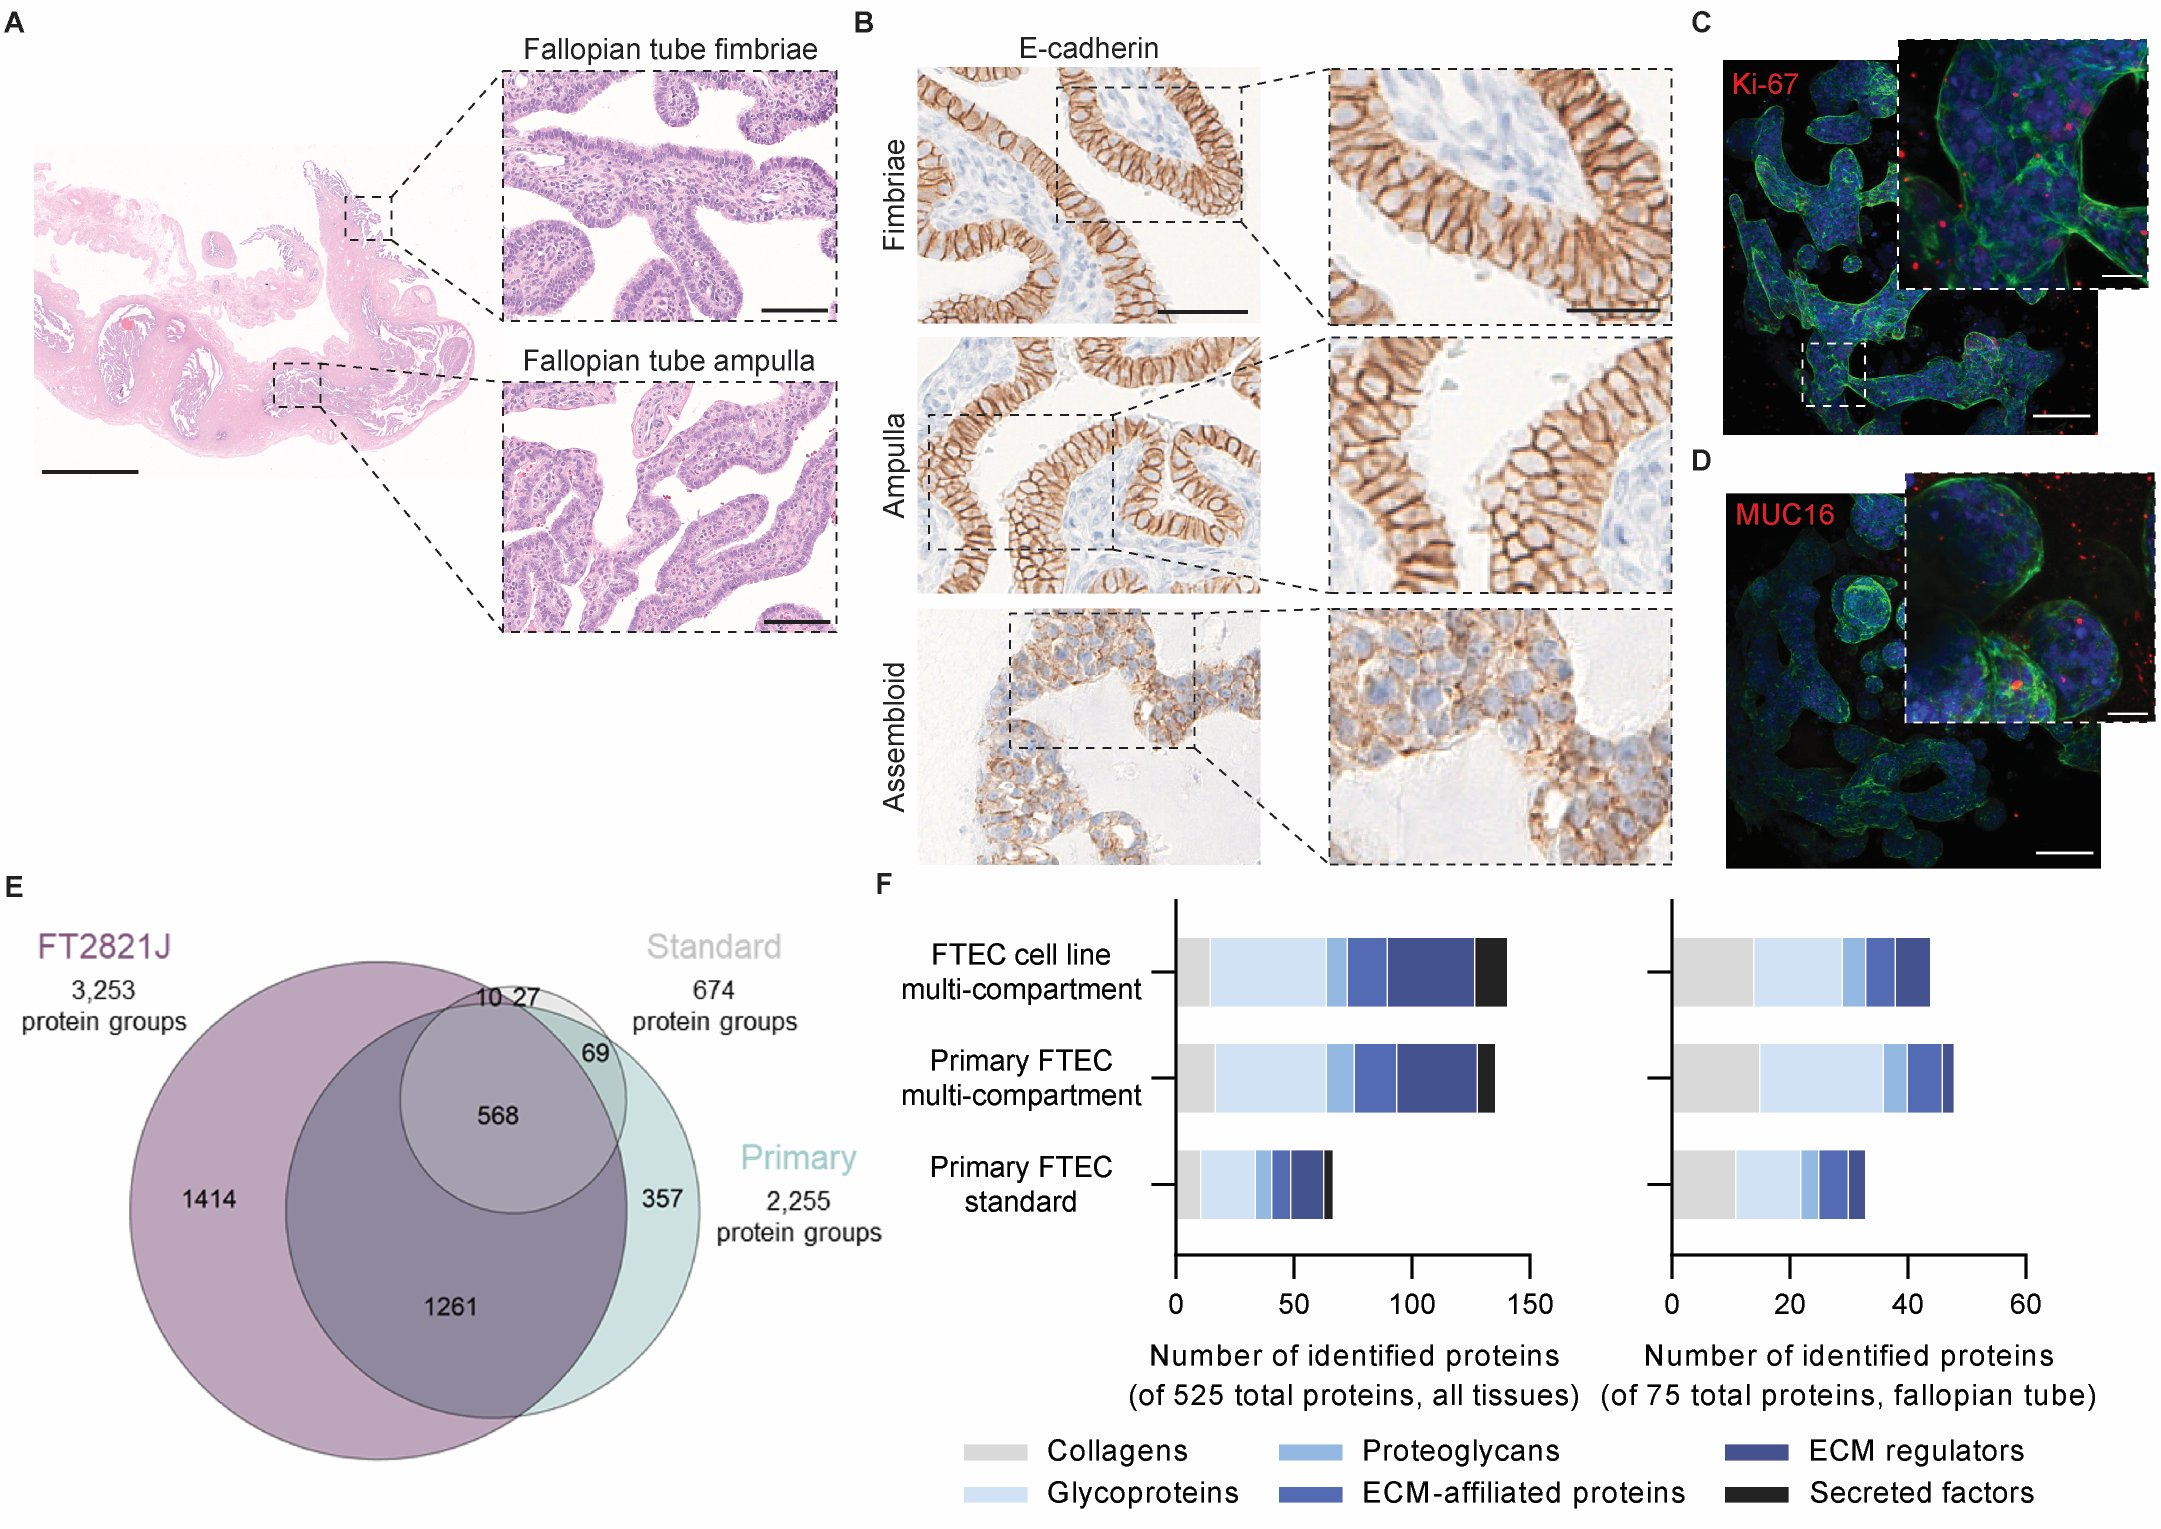
\includegraphics[width=1\textwidth,height=0.85\textheight,keepaspectratio,clip,page=1]{figures/chapter4/fig_2.jpg}
            \captionsetup{font=small}
            \caption{\textbf{Fallopian tube assembloids maintain tissue expression patterns.} (A) H\&E image of a fallopian tube tissue section. Nuclei (purple), ECM and cytoplasm (pink). Scale bar, 5 mm. Top inset is the fallopian tube fimbriae and bottom inset is the fallopian tube ampulla. Inset scale bars, 100 µm. (B) E-cadherin IHC of FFPE tissue sections of the fallopian tube fimbriae (top), fallopian tube ampulla (middle) and fallopian tube assembloid (bottom). Scale bar, 50 µm. Inset, 25 µm. Immunofluorescence staining for (C) Ki-67, and (D) MUC16 in multi-compartment fallopian tube assembloids. Images of assembloids are maximum intensity projections of stacks of confocal microscopy images. Scale bars, 100 µm. Inset scale bars, 20 µm. F-actin (green), nuclear DNA (blue), and protein of interest (red). (E) Venn diagram performed on all quantifiable protein groups (with ≥ 2 unique peptides) in FTEC cell line (purple) and primary FTEC (green) multi-compartment organoids and standard (light grey) organoids. (F) Some proteins identified in the proteomes are categorized in the human matrisome (50) for all tissues (left) and fallopian tube specific (right). (E)-(F) N = 4.}
            \label{chapter4_fig2}
        \end{center}
    \end{figure}

    \begin{figure}[p]
        \begin{center}
            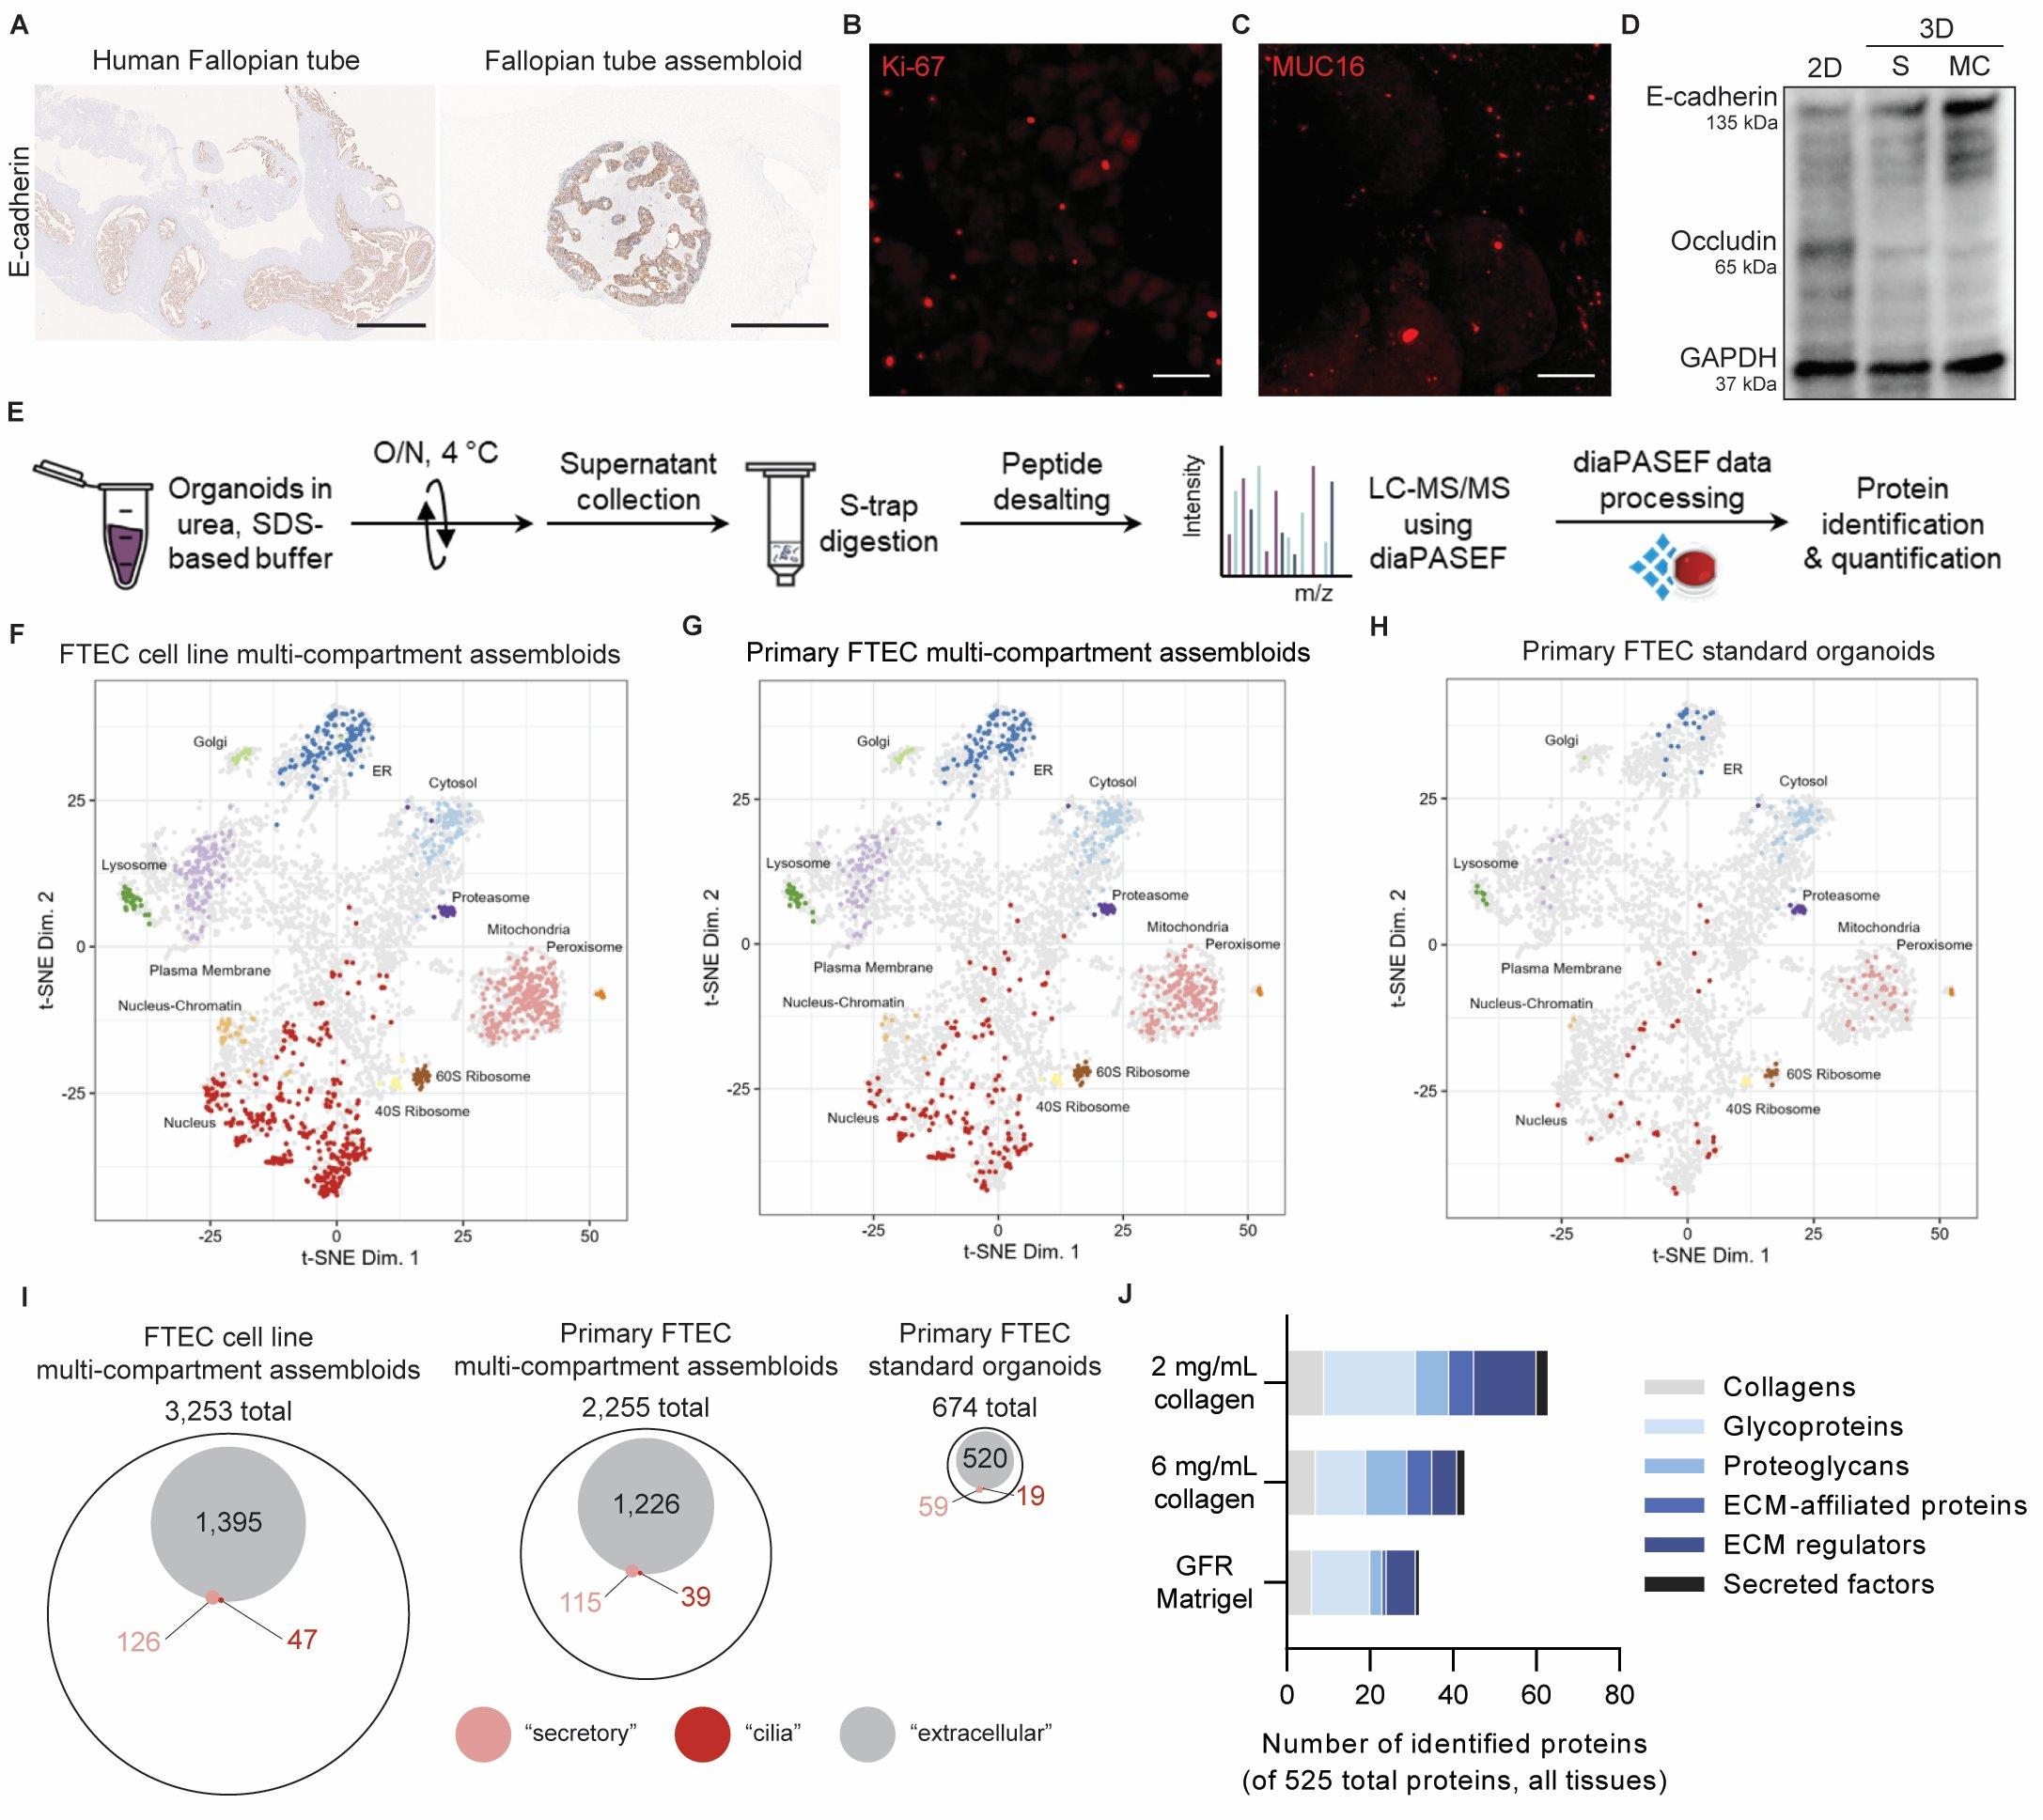
\includegraphics[width=1\textwidth,height=0.85\textheight,keepaspectratio,clip,page=1]{figures/chapter4/fig_S2.jpg}
            \captionsetup{font=small}
            \caption{\textbf{Molecular expression patterns of multi-compartment assembloids and standard organoids.}(A) FFPE tissue sections IHC stained for E-cadherin. Whole, healthy transplantation-quality tissue sections of the fallopian tube (left) and the multi-compartment assembloid (right). Scale bars, 4 mm (left) and 300 µm (right). Isolated protein of interest channel for immunofluorescence images staining (B) Ki-67, and (C) MUC16 in multi-compartment fallopian tube assembloids. Images are maximum intensity projections. Scale bars, 20 µm. (D) Global protein expression in 2D and 3D (S = standard, MC = multi-compartment) culture via western blot. GAPDH is included as a loading control.  (E) Organoids were lysed in a urea SDS-based buffer overnight. Supernants containing solubilized proteins were collected and submitted to trypsin digestion using S-trap. After desalting, proteolytic peptides were analyzed on a timsTOF HT (Bruker) mass spectrometer in diaPASEF mode, and collected MS data were processed using library-free directDIA (Biognosys) for identification and quantification. Subcellular localization of (F) FTEC cell line multi-compartment assembloid, }
            \label{chapter4_figS2}
        \end{center}
    \end{figure}
    
    \begin{figure}[h!]
        \ContinuedFloat
        \captionsetup{font=small}
        \caption[]{ (G) primary FTEC multi-compartment assembloid, and (H) primary FTEC standard organoid proteins via LOPIT map (48, 49, 54, 55). (I) Total protein groups with at least two unique peptides in FTEC cell line multi-compartment assembloids (left), primary FTEC multi-compartment assembloids (middle) and primary FTEC standard organoids (right), and the protein groups with secretory (pink), cilia (red) and extracellular (gray) Gene Ontology (52, 53) cellular components. (J) Proteins identified in the ECM control proteome are categorized in the human matrisome (50) for all tissues. (F)-(J) N = 4.}
    \end{figure}
    
    \subsection{Epithelial differentiation can be stimulated in multi-compartment assembloids}
    The fallopian tube epithelium is composed of a mixture of ciliated and secretory epithelial cells, which have key roles in oocyte transport and survival, respectively\cite{yuan2021a,suarez2021a,wanggren2008a}. IHC analysis of healthy fallopian tube tissue revealed a mixture of PAX8-positive (secretory) and PAX8-negative (ciliated)\cite{kessler2015a,perets2013a,chaves-moreira2022a,karst2011a,karst2012a} epithelial cells (Fig. 3A, fig. S3A). However, most FTECs in the assembloid were PAX8-positive. By transmission electron microscopy (TEM), we identified secretory epithelial cells and cells with cilia or microvilli facing the Matrigel region of the assembloid (Fig. 3B), resembling the lumen of the fallopian tube\cite{kessler2015a}. Tight junctions formed between epithelial cells at the assembloid-Matrigel (lumen-like) and assembloid-collagen I (stroma-like) interfaces, but epithelial secretions and cilia or microvilli were only found at the Matrigel interface (lumen-like) (Fig. 3B,C), matching the tissue anatomy. By contrast, standard organoids also formed tight junctions and showed both cilia and secretions (fig. S3B); however, in standard organoids, cilia or microvilli could be found at multiple locations on both the organoid interior (lumen-like) and exterior (stroma-like) interfaces. 
    While IHC demonstrated that most of the FTECs in the assembloid were secretory, TEM revealed that some assembloid epithelial cells could become ciliated. Secretory FTECs can differentiate into ciliated FTECs upon hormone stimulation\cite{fitzgerald2019a,donnez1985a,comer1998a,comer1998a,garcia-alonso2021a}, so we treated our assembloids with \textbeta-estradiol (E2) and progesterone (P4), two steroid hormones of the menstrual cycle that elicit morphological and functional responses from the fallopian tube epithelium (67). The resulting molecular response was measured via RT-qPCR (Fig. 3D). We observed overall increases in estrogen receptor 1 (ESR1) expression with \textbeta-estradiol treatment and a slight increase with progesterone treatment, matching previously reported responses in fallopian tube tissue\cite{brodowska2021a} and mouse FTEC standard organoids\cite{xie2018a}. In the follicular phase when estrogen is high and progesterone is low \cite{monis-a}, progesterone receptor levels increase in the fallopian tube epithelium\cite{akison2012a} and, accordingly, progesterone receptor (PGR) expression increased when our assembloids were treated with \textbeta-estradiol. \textbeta-estradiol treatment also caused a decrease in the relative expression of secretory cell marker PAX8, which is evidence of ciliated FTEC differentiation (Fig. 3E). The relative expression of markers related to cilia motility/regulatory transcription factor (FOXJ1)\cite{yu2008a,turco2017a} and stem cell differentiation into ciliated cells (OLFM4)\cite{gu2020a,li2020a} also increased with \textbeta-estradiol stimulation. The relative expression of MKI67 was not significantly changed from the untreated control (Fig. 3F), which aligns with previous reports of null or limited proliferation of oviductal epithelium when stimulated with estradiol\cite{eddie2015a,moyle-heyrman2016a}. Standard organoids did not always produce these expected responses to hormone treatment (fig. S3C). The relative expression of MKI67 was significantly reduced when treated with progesterone, and markers of morphological cell type (PAX8, FOXJ1) were unchanged from controls with \textbeta-estradiol stimulation (fig. S3D). Progesterone also prompted an unexpected increase in TNF expression. These results demonstrated a physiological response to steroid hormone stimulation by the healthy fallopian tube assembloid, and that the ratio of ciliated:secretory epithelial cells in multi-compartment assembloids can be tuned to better match the composition of the tissue epithelium.
    While cilia and smooth muscle are both involved in the transport of an oocyte through the fallopian tube, motile cilia are especially important when capturing and initiating oocyte transport in the infundibulum region near the ovary\cite{yuan2021a,suarez2021a,wanggren2008a}. Cilia are vital to a functional fallopian tube, and thus, cilia must be present in an assembloid aiming to capture the physiological fallopian tube. As an additional confirmation of ciliation potential, we identified Gene Ontology\cite{ashburner2000a,Ashburner2000Gene} biological processes that were upregulated when multi-compartment assembloids were treated with \textbeta-estradiol via diaPASEF-MS-based proteomics\cite{meier2020a} and ConsensusPathDB\cite{kamburov2011a,kamburov2011a} (Fig. 3G-I). This analysis was performed on cell line (Fig. 3G) and primary (Fig. 3H) multi-compartment assembloids to demonstrate the functional capacity of the assembloid model with cells from multiple sources. For each condition, the average coefficient of variation (CV) across biological replicates in the proteomics dataset ranged between 20\% and 39\% at the protein level (fig. S3E), demonstrating good reproducibility for large-scale discovery and quantitative analytical assays that monitor thousands of proteins. HSPG2 was among the protein groups upregulated in both primary and cell line assembloids stimulated with \textbeta-estradiol, which has been linked to reproductive functions including tissue development and blastula implantation\cite{chen2023a,garcia2024a}.  \textbeta-estradiol stimulation also resulted in upregulation of cytoskeleton-related biological processes including cytoskeleton organization and epithelial cell differentiation (FT2821J cell line) and plasma membrane bounded cell projection organization and cell motility/migration (primary) (Fig. 3I). Among other processes regarding epithelial cell junction and ECM/basement membrane assembly, these upregulated biological processes confirm assembloid epithelial maturation upon \textbeta-estradiol stimulation, including the differentiation of secretory cells into ciliated cells and cilia motility\cite{park2008a,antoniades2014a,garcia2018a}.

    \begin{figure}[p]
        \begin{center}
            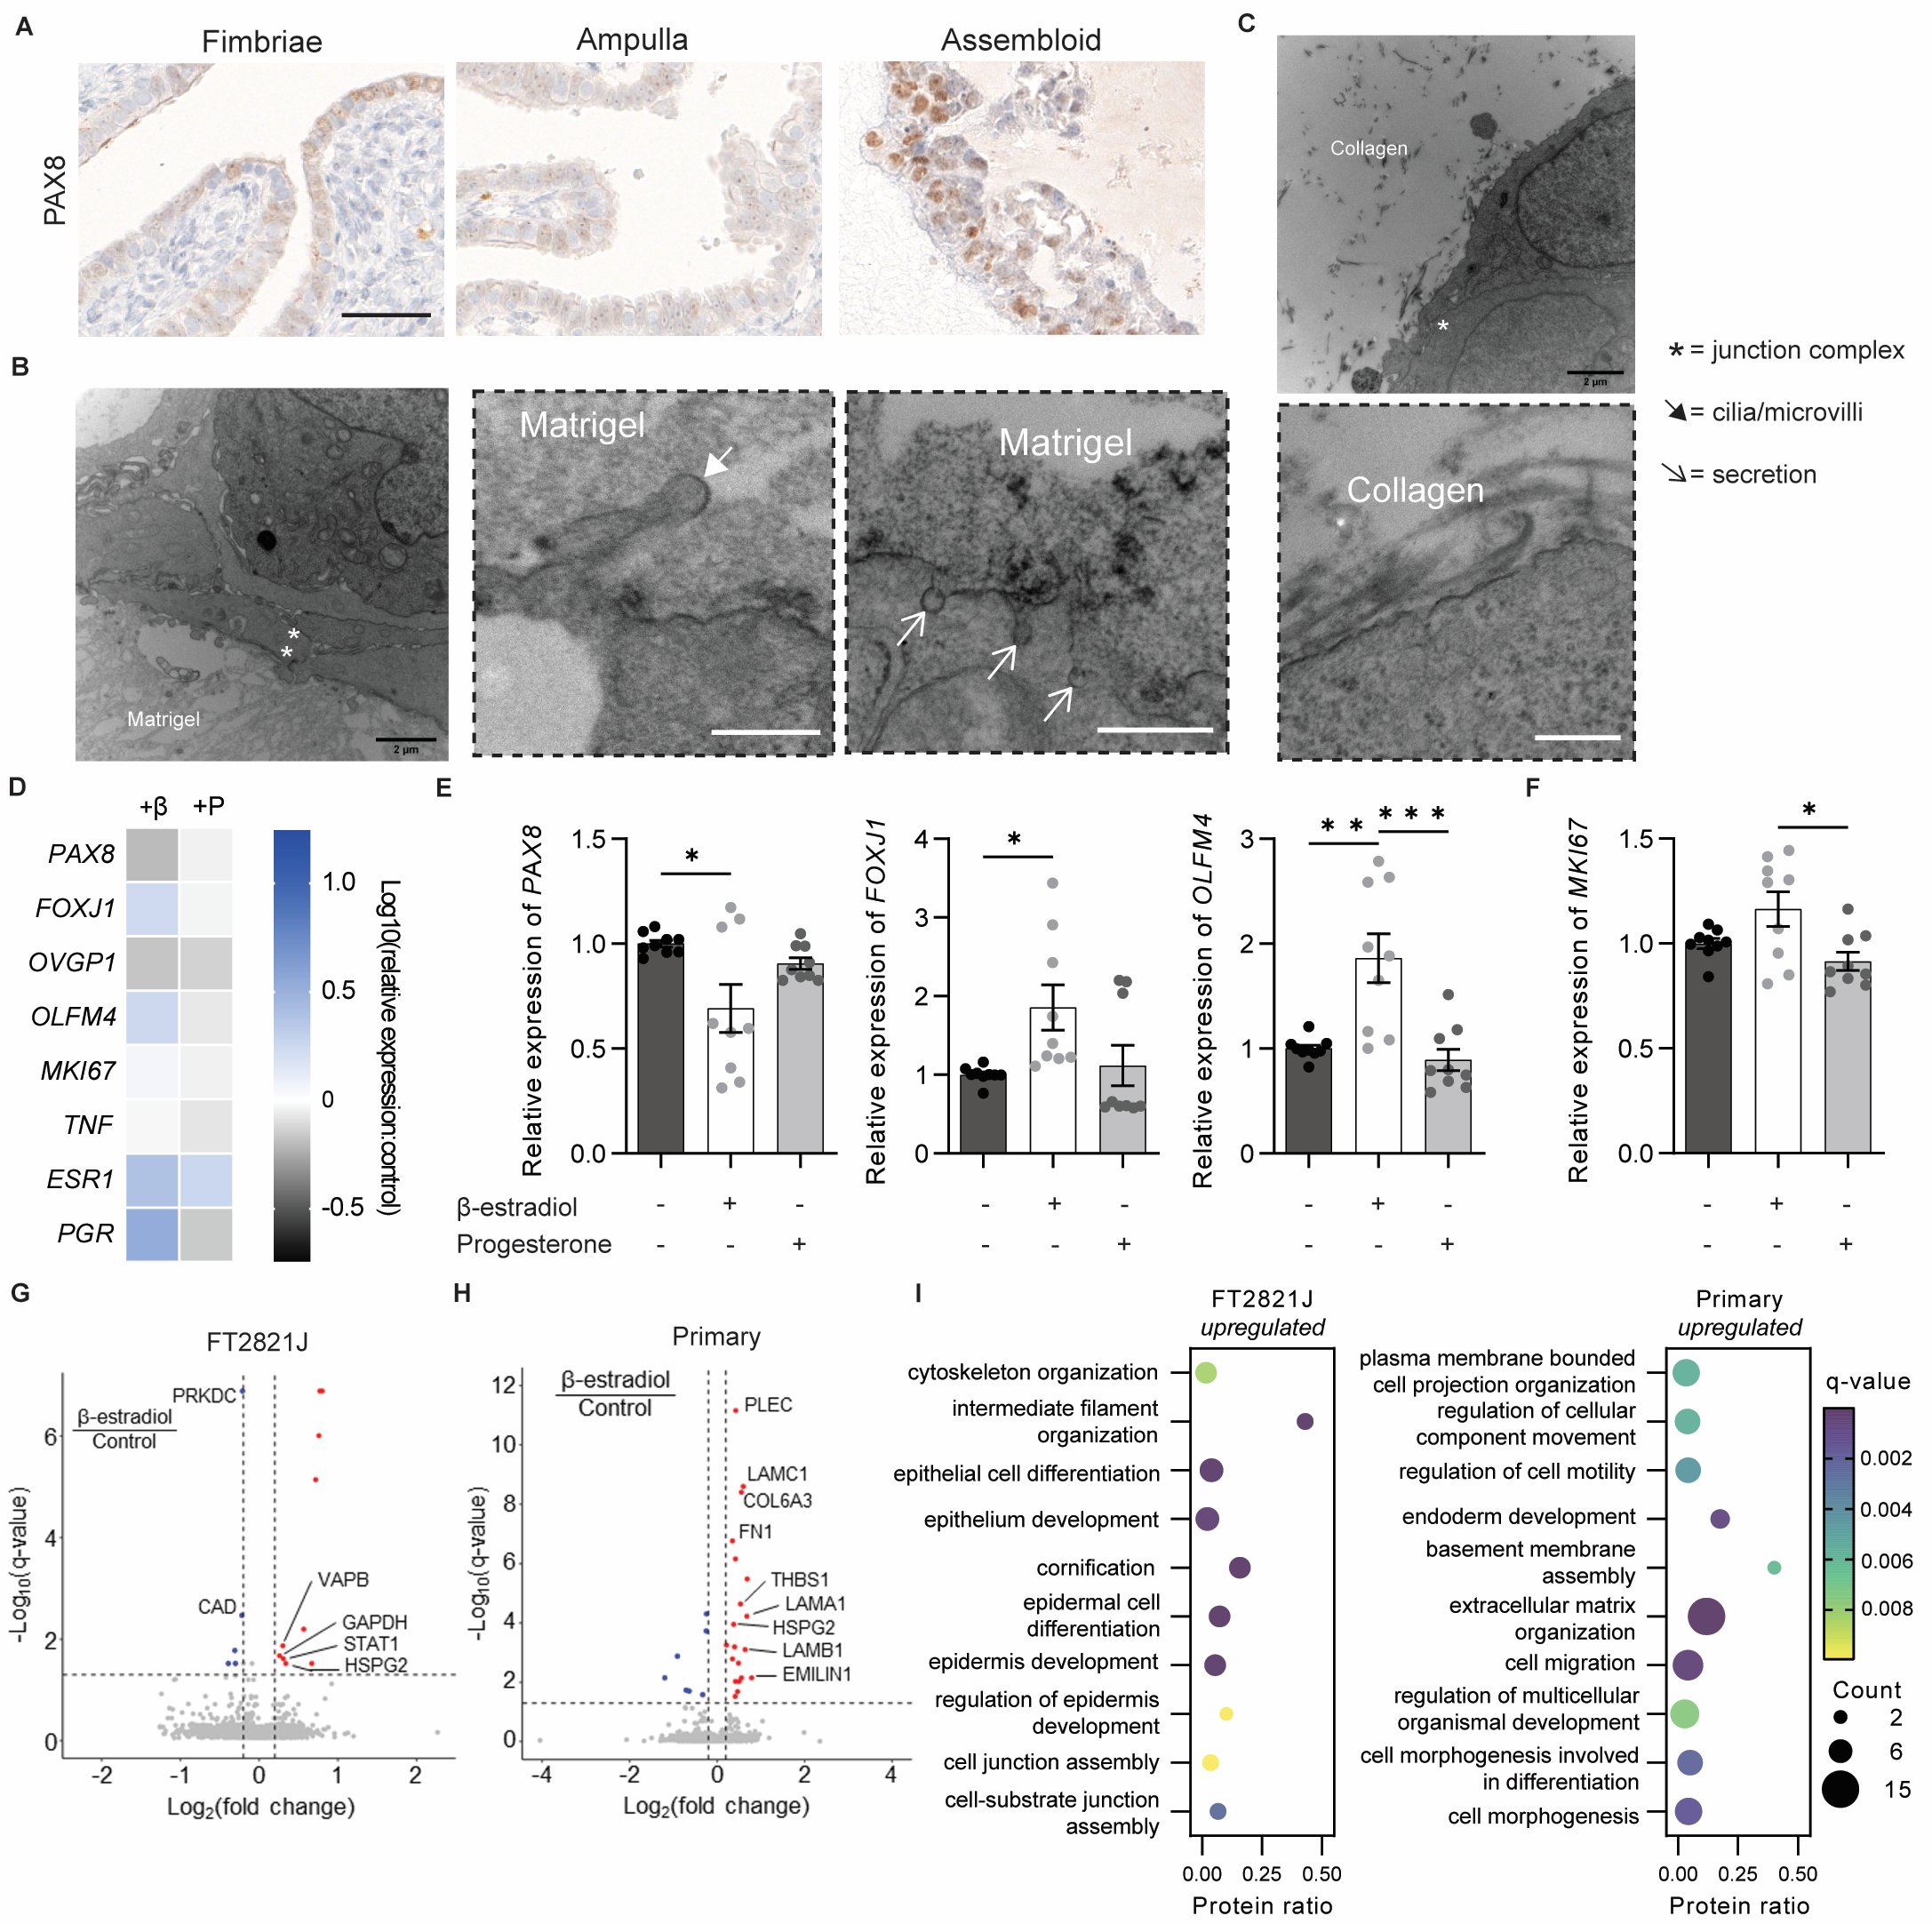
\includegraphics[width=1\textwidth,height=0.85\textheight,keepaspectratio,clip,page=1]{figures/chapter4/fig_3.jpg}
            \captionsetup{font=small}
            \caption{\textbf{Epithelial composition of multi-compartment assembloids.} (A) PAX8 IHC of FFPE tissue sections of the fallopian tube fimbriae (top), fallopian tube ampulla (middle) and fallopian tube assembloid (bottom). Scale bar, 50 µm.  TEM of the (B) cell-Matrigel (lumen-like) interface and (C) cell-collagen I (stroma-like) interface of a multi-compartment assembloid. Scale bars, 2 µm. Inset scale bars, (B) 500 nm (both) and (C) 300 nm. Asterisk = junction complex, filled arrow = cilia/microvilli, open arrow = secretion. (D) RT-qPCR of β-estradiol (β) or progesterone (P) treated multi-compartment assembloids. Data are log10(relative expression:untreated control). Relative expression of genes related to (E) ciliated differentiation and (F) proliferation. }
            \label{chapter4_fig3}
        \end{center}
    \end{figure}
    
    \begin{figure}[h!]
        \ContinuedFloat
        \captionsetup{font=small}
        \caption[]{(D)-(F) N = 3, n = 3. Statistical tests: one-way ANOVA with multiple comparisons, ***P $≤$ 0.001, **P $≤$ 0.01, *P ≤ 0.05. All data are mean $±$ SEM. Volcano plot of upregulated (red)/downregulated (blue) protein groups when (G) FTEC cell line multi-compartment assembloids and (H) primary FTEC multi-compartment assembloids were treated with \textbeta-estradiol (statistical significance: q-value $≤$ 0.05 and absolute log2(fold-change) $≥$ 0.2). (I) Gene Ontology\cite{Ashburner2000Gene, ashburner2000a} biological processes that were upregulated in \textbeta-estradiol treated FTEC cell line (left) and primary FTEC (right) multi-compartment assembloids. Relative protein quantification assessed by DIA-MS (47) and subsequent enrichment analysis performed using ConsensusPathDB\cite{kamburov2009a,kamburov2011a}. N = 4.}
    \end{figure}

    \begin{figure}[p]
        \begin{center}
            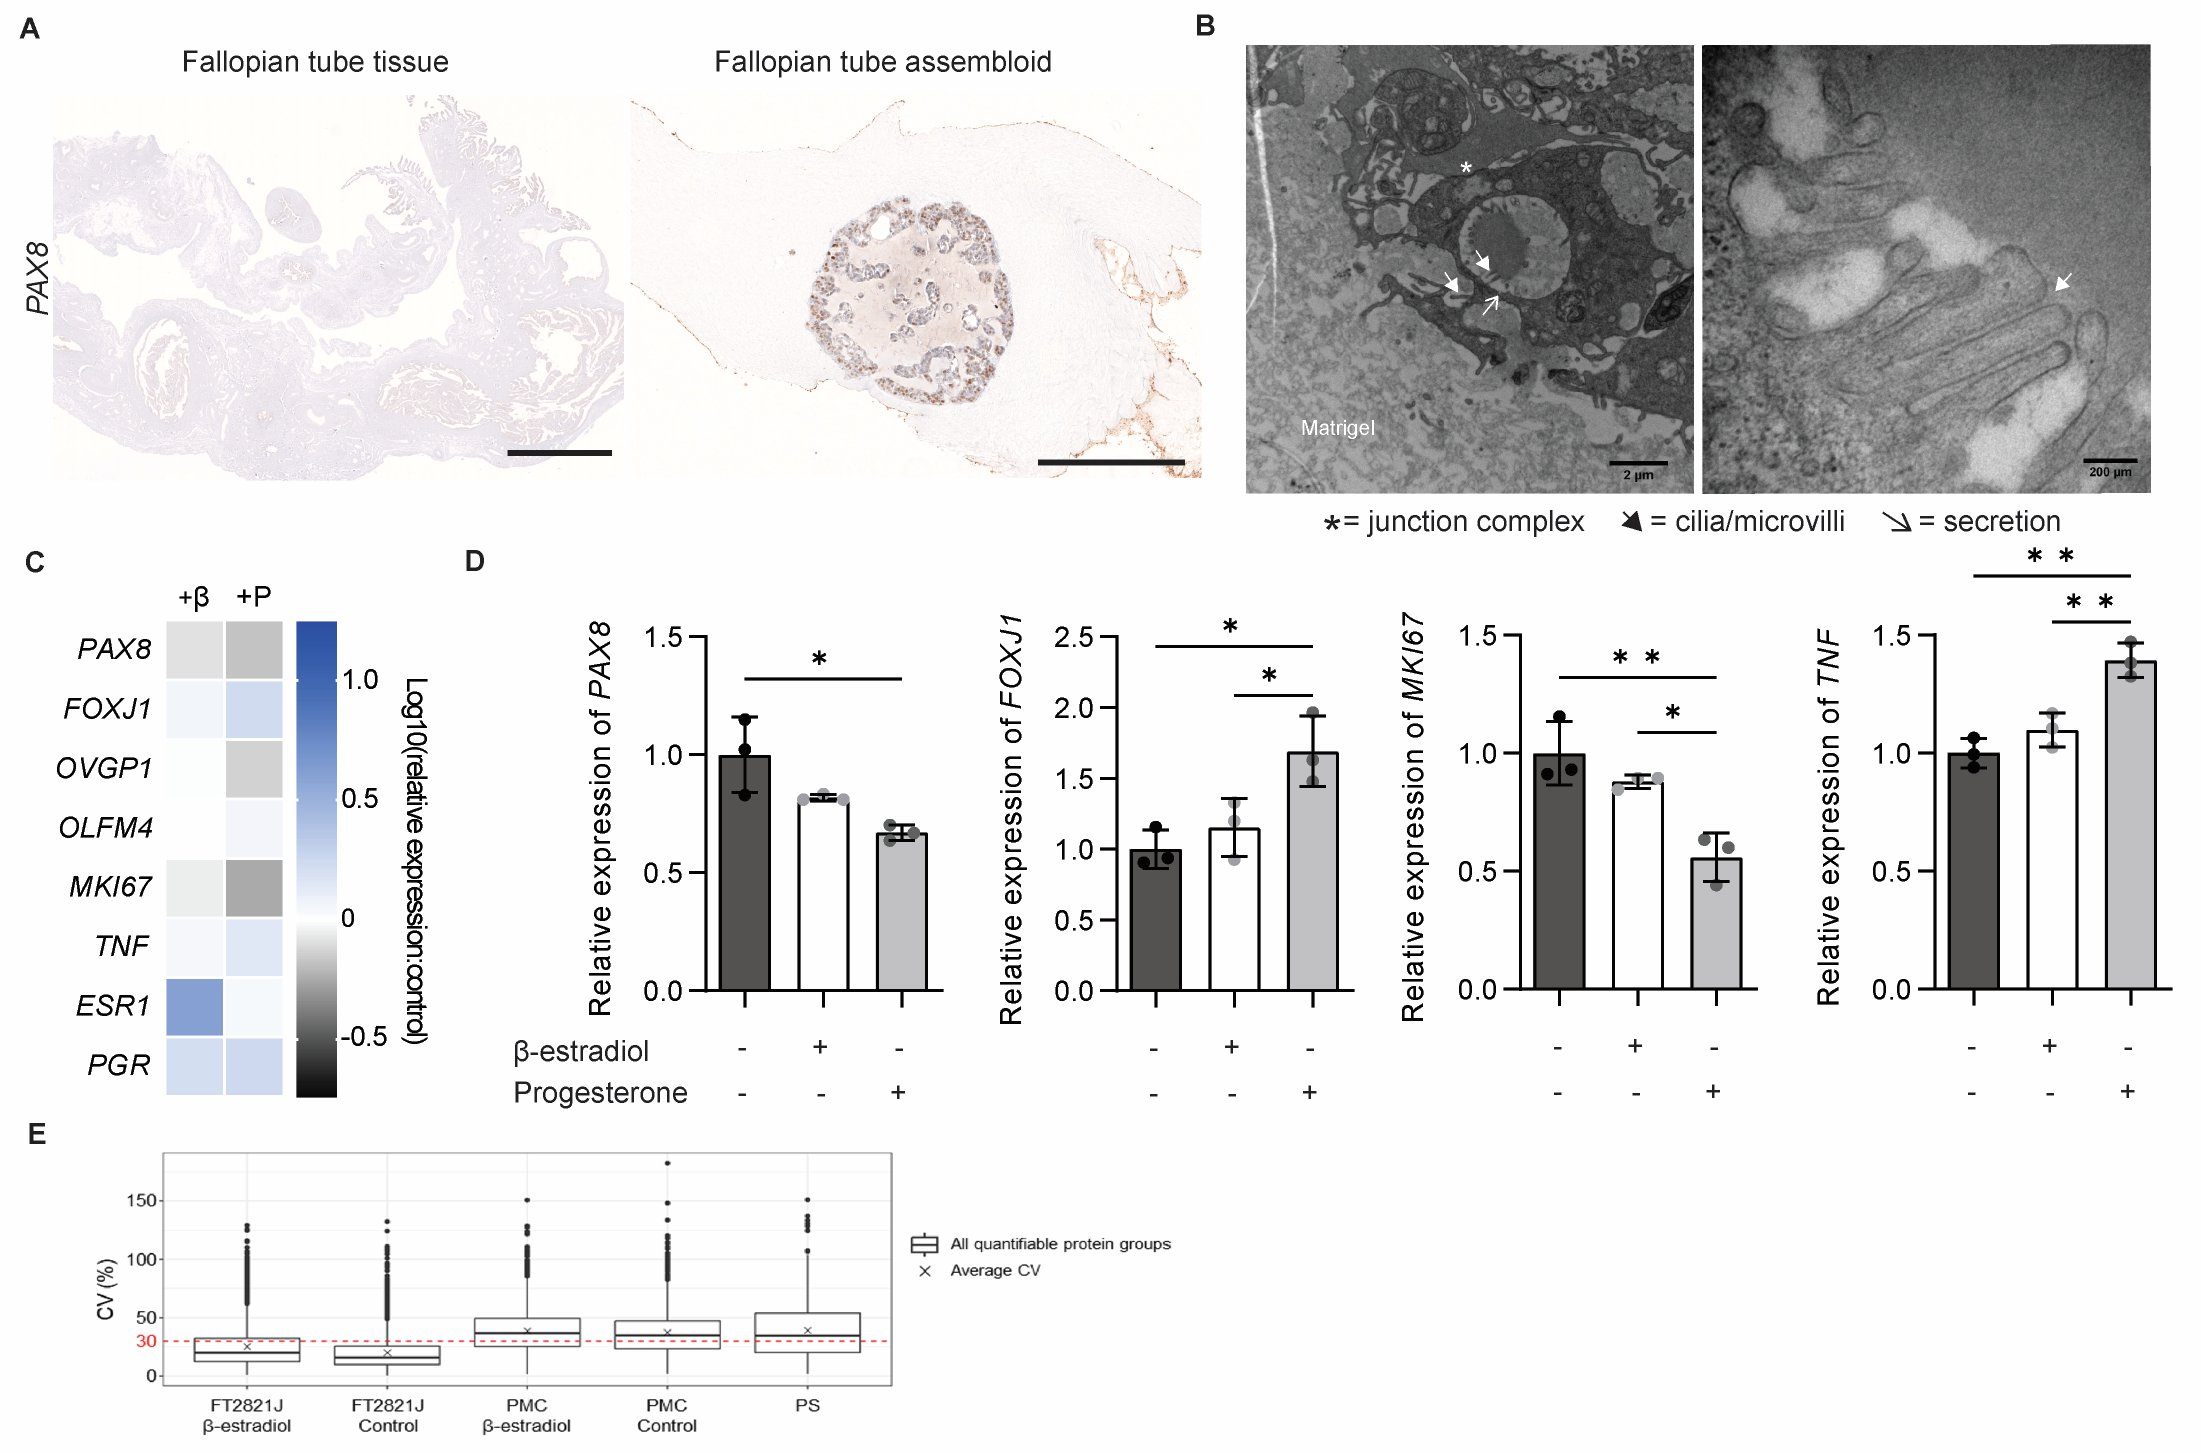
\includegraphics[width=1\textwidth,height=0.85\textheight,keepaspectratio,clip,page=1]{figures/chapter4/fig_S3.jpg}
            \captionsetup{font=small}
            \caption{\textbf{Epithelial composition of the fallopian tube in vitro models.} (A) FFPE tissue sections IHC stained for PAX8. Whole, healthy transplantation-quality tissue sections of the fallopian tube (top) and the multi-compartment assembloid (bottom). Scale bars, 4 mm (top) and 300 µm (bottom). (B) Transmission electron microscopy of a standard fallopian tube organoid. Scale bar, 2 µm (left) and 200 nm (right). Asterisk = junction complex, filled arrow = cilia/microvilli, open arrow = secretion. (C) RT-qPCR of β-estradiol (β) or progesterone (P) treated standard organoids. Data are log10(relative expression:untreated control). (D) Relative expression of genes related to cell differentiation into ciliated epithelial cells and proliferation in standard organoids. Data are mean ± SD. Statistical test: one-way ANOVA with multiple comparisons, **P ≤ 0.01, *P ≤ 0.05.  (C)-(D) N = 1, n = 3. (E) Coefficients of variation (CVs) were calculated on the protein group abundance of four replicates. The boxplots display the CV distribution obtained for the FTEC cell line multi-compartment organoids (FT2821J), primary FTEC multi-compartment organoids (PMC) and primary standard organoids (PS), using all quantifiable protein groups (with ≥ 2 unique peptides). Good reproducibility using diaPASEF-MS was achieved among organoid replicates (n = 4), with overall average CVs ranging between 20\% and 39\%, which is compatible with large-scale discovery and quantification assays. N = 4.}
            \label{chapter4_figS3}
        \end{center}
    \end{figure}
    
    % \begin{figure}[h!]
    %     \ContinuedFloat
    %     \captionsetup{font=small}
    %     \caption[]{ (G) primary FTEC multi-compartment assembloid, and (H) primary FTEC standard organoid proteins via LOPIT map (48, 49, 54, 55). (I) Total protein groups with at least two unique peptides in FTEC cell line multi-compartment assembloids (left), primary FTEC multi-compartment assembloids (middle) and primary FTEC standard organoids (right), and the protein groups with secretory (pink), cilia (red) and extracellular (gray) Gene Ontology (52, 53) cellular components. (J) Proteins identified in the ECM control proteome are categorized in the human matrisome (50) for all tissues. (F)-(J) N = 4.}
    % \end{figure}
    
    \subsection{Activated multi-compartment assembloids reproduce the function of the organ}
    From a functional perspective, the differentiation of FTECs into ciliated epithelial cells in response to \textbeta-estradiol stimulation is important. Cilia need to be expressed in the epithelium, and these cilia need to also be motile and able to transport an object (oocyte) along the epithelium\cite{yuan2021a,suarez2021a,wanggren2008a}. To test the function of cilia induced by \textbeta-estradiol treatment and demonstrate the multi-compartment fallopian tube assembloid’s mechanical function, we developed a bead displacement assay where oocyte-mimicking fluorescent microbeads were mixed in the lumen-like region of assembloids (Fig. 4A). Some of these assembloids were stimulated with \textbeta-estradiol to induce ciliated differentiation of their epithelial cells. After 7 days of growth the assembloids had matured, and microbeads transported along the interface of the assembloid epithelium and the lumen-like region were tracked using time-lapse confocal microscopy (Fig. 4B, Video S1). The trajectories of beads were more irregular and covered larger distances when assembloids were treated with \textbeta-estradiol than in untreated controls (Fig. 4C). The stimulated trajectories were much larger than cell movement within the assembloids or the system noise without any cells, and followed the curvature of the assembloid epithelium. This was quantitatively verified by calculating the mean squared displacements (MSDs) of the microbeads over 8h (Fig. 4D) and the microbead velocity (Fig. 4E)\cite{wirtz2009a,wu2015a}. While there was no significant difference in the persistence of microbead movement from the untreated control (persistence time), the total microbead diffusivity was increased in the \textbeta-estradiol treated condition (fig. S4A). 
    The RT-qPCR and DIA-MS proteomics results presented earlier (Fig. 3D-G) indicated an increase in ciliated cells when these assembloids were treated with \textbeta-estradiol. As an additional confirmation that the increase in microbead movement could be due to motile cilia, \textbeta-estradiol treated and untreated assembloids were digested, cells were isolated from assembloid debris, and cell motility in DPBS was tracked (Fig. 4F, Video S2). If cells had motile cilia, the cilia acted as a motor propelling suspended cells through DPBS\cite{garcia2018a} (Fig. 4G). Cells isolated from \textbeta-estradiol treated assembloids had higher MSDs than cells isolated from the untreated assembloids (Fig. 4H). Together, the data collected from \textbeta-estradiol stimulated assembloids via RT-qPCR, DIA-MS proteomics, and the cilia-driven motility assay concluded that the increased microbead movement observed in \textbeta-estradiol stimulated assembloids was the result of functional cilia along the assembloid epithelium-lumen interface. Thus, multi-compartment assembloids capture the organ’s mechanical function.
    The same bead displacement assay was performed in standard organoids (fig. S4B). Individual standard organoids grow from a single parent cell where a lumen forms in the center of an individual organoid\cite{kessler2015a}. Due to the nature of organoid maturation in the standard model, standard organoids either encased microbeads in the organoid lumen-like region or contacted microbeads along the external epithelial surface (fig. S4C). However, our electron microscopy results had previously revealed that standard organoids can form cilia or microvilli on the lumen-like and external epithelial surfaces (fig. S3B), so microbeads in contact with any surface of the organoid could be moved by cilia if the cilia were motile. The trajectories of beads tracked in standard organoids revealed larger trajectories in the untreated organoids than in those treated with \textbeta-estradiol (fig. S4D). The quantification of these trajectories also showed little difference in the microbead velocities of any experimental group (fig. S4E); although, microbead MSDs in untreated organoids were increased compared to the noise of the system (fig. S4F). There was no statistically significant difference in the persistence time or total diffusivity for the microbeads tracked in these experimental groups (fig. S4G). Together, these results suggest that bead movement in standard organoids was more likely due to the movement of cells than motile cilia induced by hormone stimulation.
    These functional assessments demonstrate that the multi-compartment assembloids resemble the fallopian tube organ in both hormone response and transport ability, thus displaying functional similarity to the organ.
    
    \begin{figure}[p]
        \begin{center}
            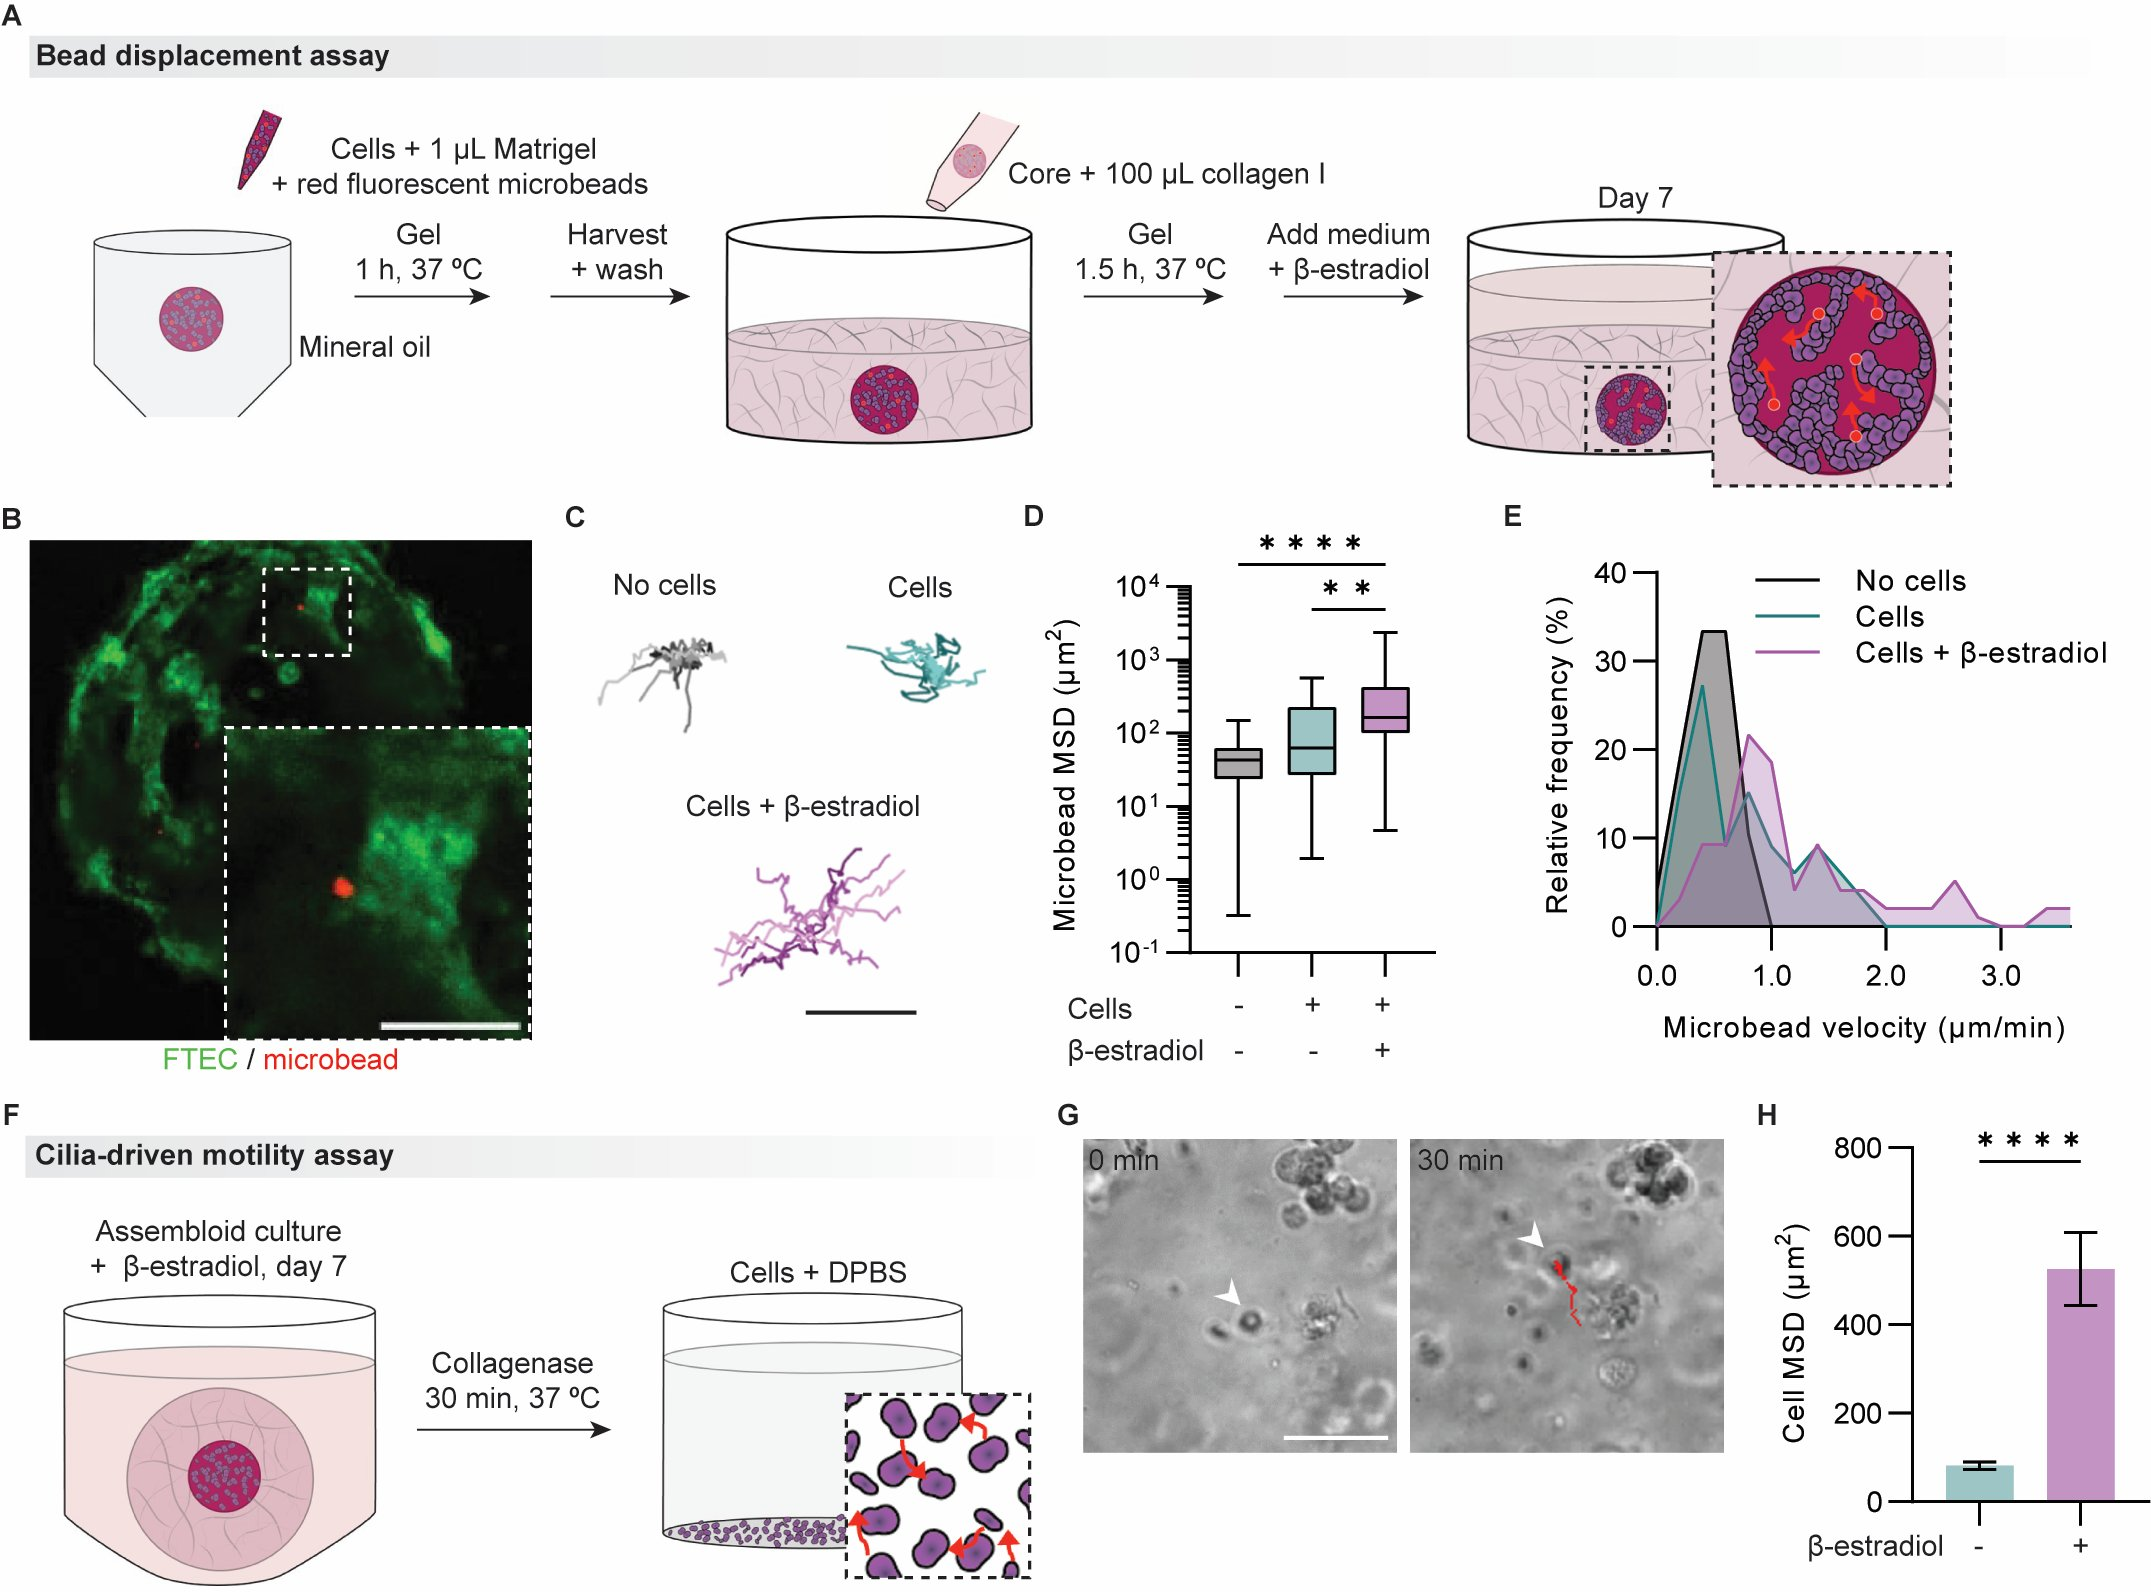
\includegraphics[width=1\textwidth,height=0.85\textheight,keepaspectratio,clip,page=1]{figures/chapter4/fig_4.jpg}
            \captionsetup{font=small}
            \caption{\textbf{Multi-compartment assembloids demonstrate functional similarity to the fallopian tube.} (A) Cartoon depicting the bead displacement assay protocol in assembloids. Arrows indicate microbead movement. (B) A multi-compartment assembloid used in the bead displacement assay with microbeads at the assembloid’s epithelial-lumen-like interface. EGFP-tagged FTECs (green) and microbeads (red). Scale bar, 100 µm. (C) Representative microbead trajectories from assembloid cores with microbeads only (noise, black), microbeads with FTECs (teal), and microbeads with FTECs treated with β-estradiol (purple). Scale bar, 10 µm. (D) Microbead MSDs over 8 h. Center line, median; box limits, upper and lower quartiles; whiskers, min to max. (E) Relative frequency of microbead velocities. (C)-(E) N = 3, n = 4-46. (F) Cartoon depicting cilia motility assay with assembloid digestion. Arrows indicate cell movement in DPBS. (G) Phase-contrast images from the cilia-driven motility assay. Cell trajectory (red). Scale bar, 50 µm. (H) Cell MSDs in DPBS after assembloid digestion. N = 3, n > 100. Statistical tests: (D) one-way ANOVA with multiple comparisons, (H) unpaired t-test, ****P ≤ 0.0001, **P ≤ 0.01. All data are mean ± SEM. }
            \label{chapter4_fig4}
        \end{center}
    \end{figure}
    
    % \begin{figure}[h!]
    %     \ContinuedFloat
    %     \captionsetup{font=small}
    %     \caption[]{}
    % \end{figure}

    \begin{figure}[p]
        \begin{center}
            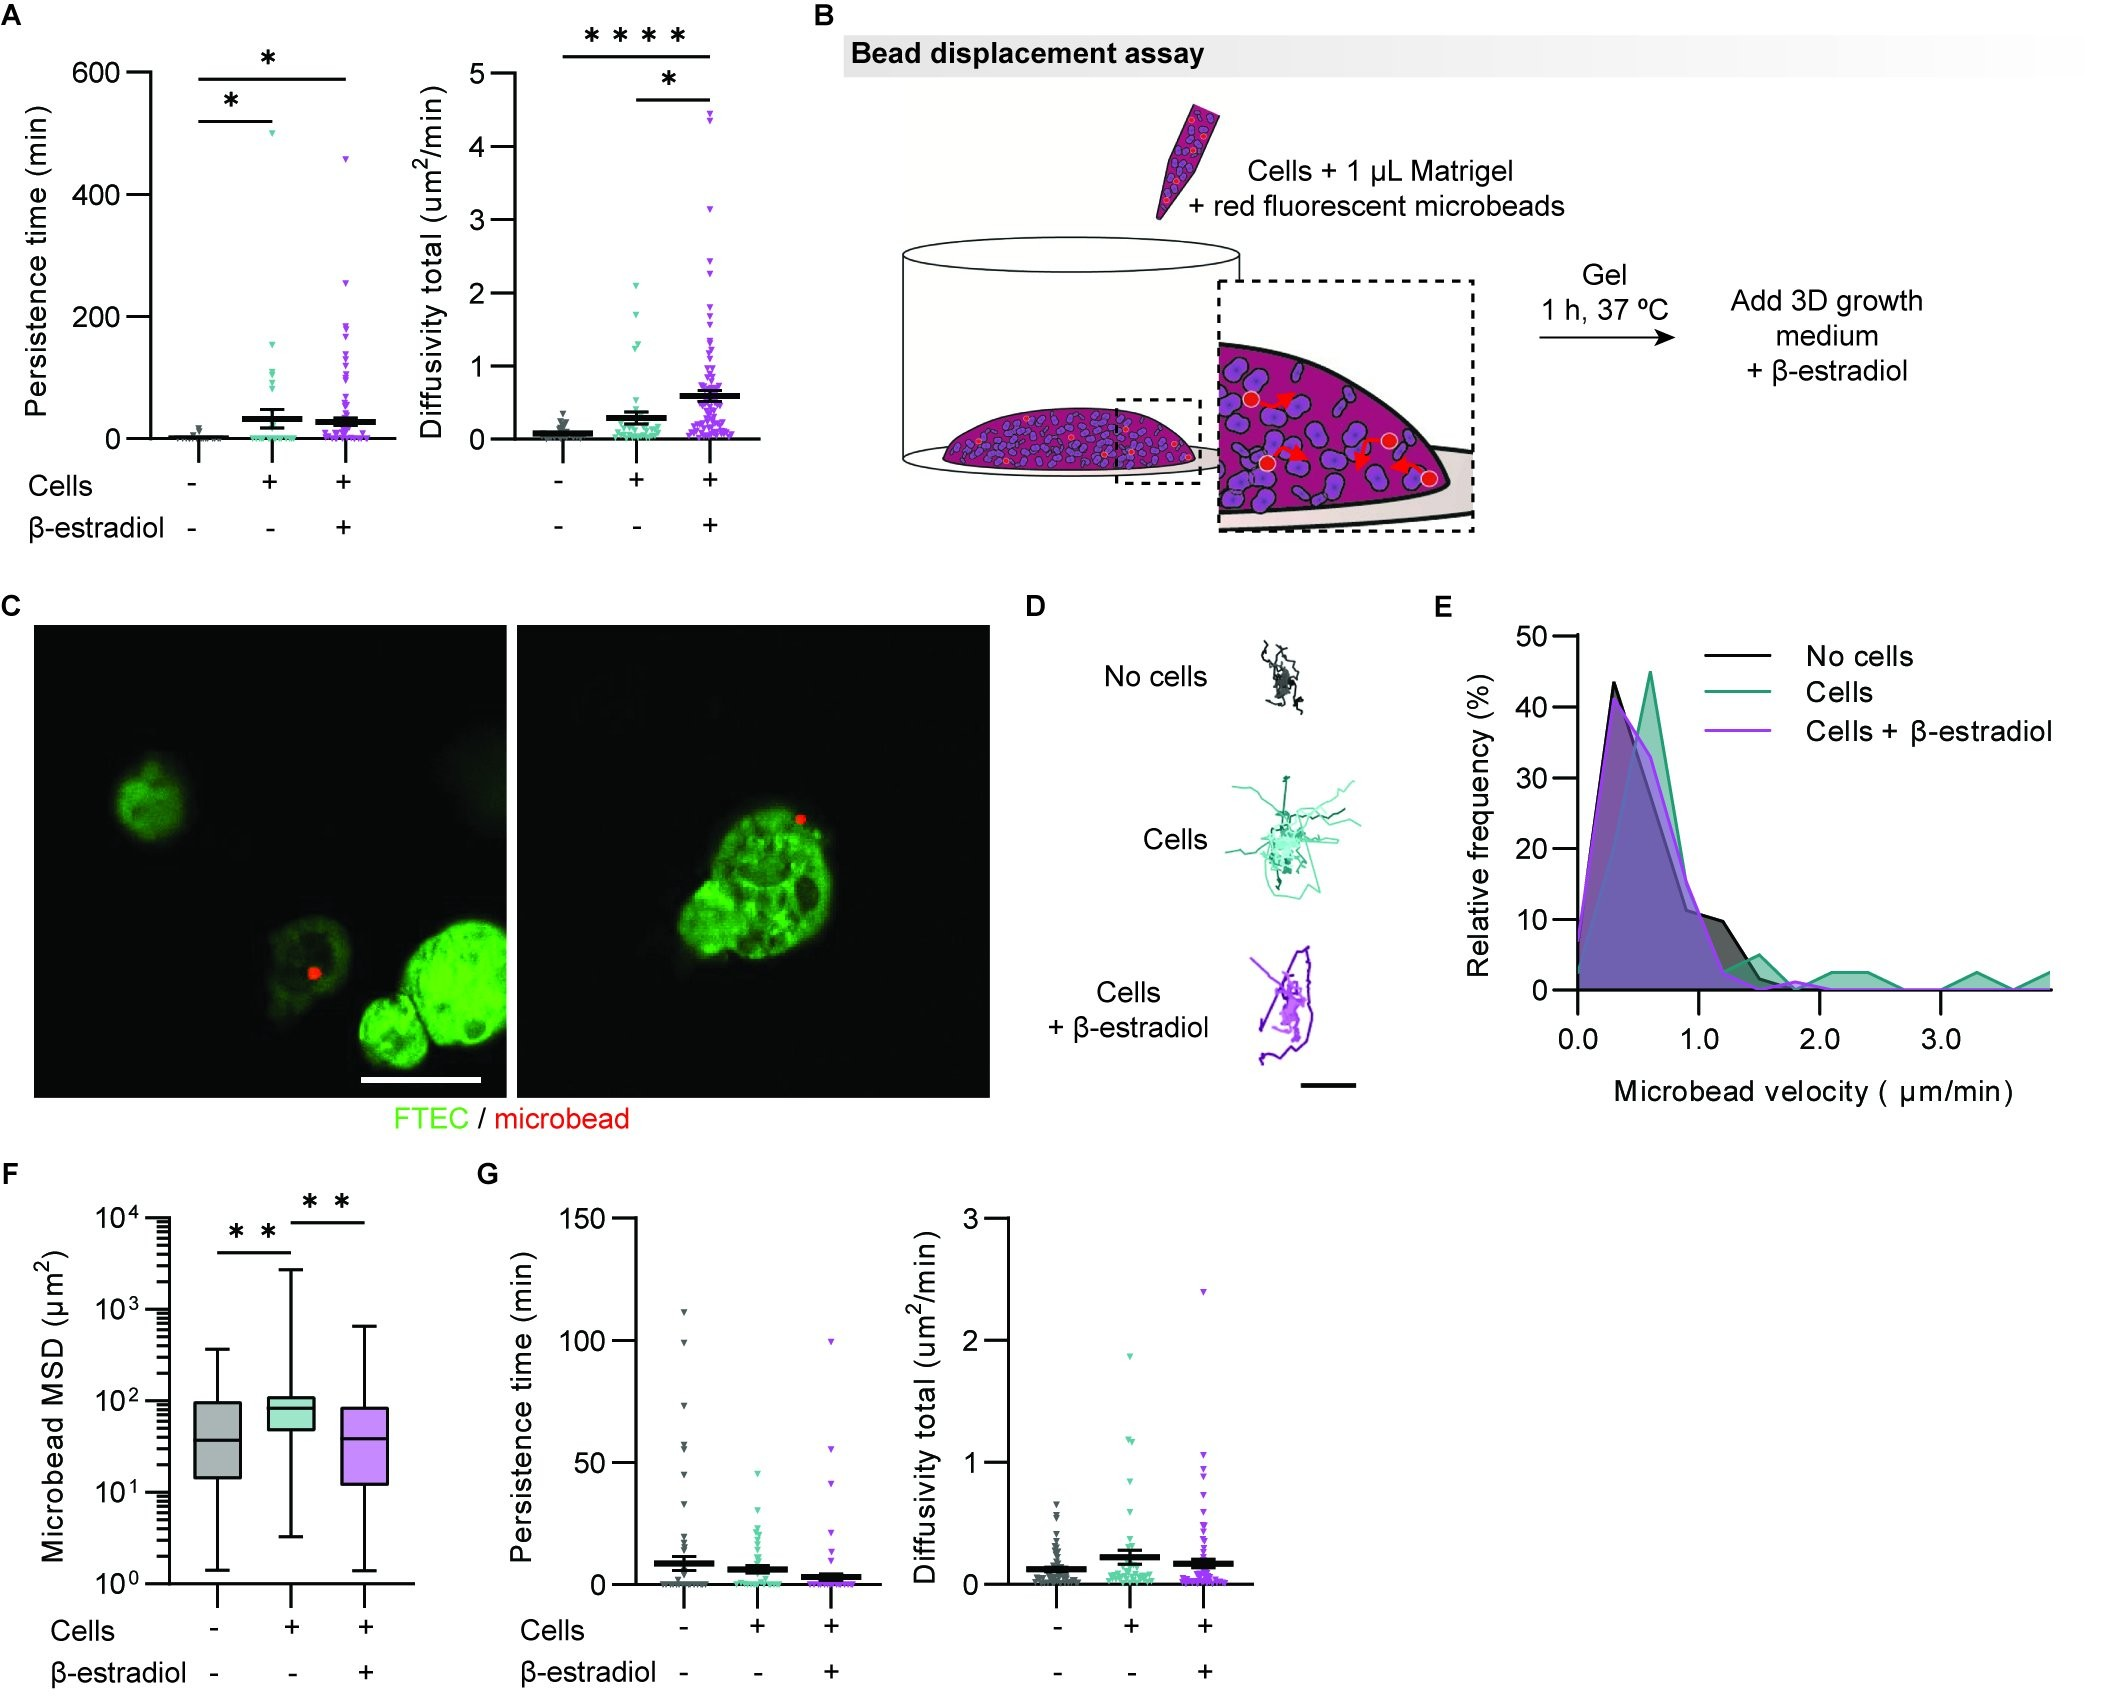
\includegraphics[width=1\textwidth,height=0.85\textheight,keepaspectratio,clip,page=1]{figures/chapter4/fig_S4.jpg}
            \captionsetup{font=small}
            \caption{\textbf{Mechanical function of ciliated epithelial cells.} (A) Persistence time and total diffusivity of microbeads in the multi-compartment bead displacement assay. N = 3, n = 4-46. (B) Cartoon depicting the bead displacement assay protocol in standard organoids. (C) A standard organoid used in the bead displacement assay with a microbead at the organoid’s epithelial interface. EGFP-tagged FTECs (green) and microbeads (red). Scale bar, 100 µm.(D) Representative microbead trajectories from standard organoids with microbeads only (noise, top), microbeads with FTECs (middle), and microbeads with FTECs treated with β-estradiol (bottom). Scale bar, 7.5 µm. (E) Relative frequency of microbead velocities in standard organoids. (F) Microbead MSD over 8 h. Center line, median; box limits, upper and lower quartiles; whiskers, min to max. (G) Persistence time and total diffusivity of microbeads in the standard organoid bead displacement assay. (D)-(G) N = 2, n = 18-45. (A) and (F)-(G) data are mean ± SEM. Statistical test: (A) and (F)-(G) one-way ANOVA with multiple comparisons, ****P ≤ 0.0001, **P ≤ 0.01, *P ≤ 0.05. }
            \label{chapter4_figS4}
        \end{center}
    \end{figure}
    
    % \begin{figure}[h!]
    %     \ContinuedFloat
    %     \captionsetup{font=small}
    %     \caption[]{}
    % \end{figure}
    
    \subsection{CODA provides architectural feedback for assembloid design iterations}
    After comprehensive evaluation of the multi-compartment assembloid model using traditional and novel in vitro assays, the assembloid model’s molecular and functional similarity to fallopian tube tissue was validated using quantitative metrics. The assembloid’s structure, however, was thus far evaluated using qualitative comparisons. To add quantitative validations of the 3D architecture of the multi-compartment assembloid, we developed a platform that rigorously compared our assembloids to a whole healthy human fallopian tube using CODA (Fig. 5A). CODA is a deep learning-based pipeline that 3D reconstructs bulk tissues at cellular resolution from serial histological sections\cite{kiemen2022a,Braxton20243D}. Here, CODA generated a 3D reference map of a whole fallopian tube received from a transplantation center from an organ donor who had no history of reproductive system disease or other history that would influence cellular architecture or function. Using this reference map, architectural measurements including the lumen volume and cell concentrations were quantified and then used to meticulously improve our assembloid model to best mimic the tissue architecture. Assembloid parameters were adjusted iteratively until this quantitative biomimetic comparison revealed marked improvement in structural biomimetic properties of our assembloid model (i.e., most quantifications were within 25\% deviation from the tissue).
    The CODA workflow was first applied to reconstruct the fallopian tube of a post-menopausal (72-year-old) female donor. Briefly, the FFPE tissue sample was serially sectioned (4 µm thickness) and one in every two sections was stained with hematoxylin and eosin (H\&E) and digitized for an axial resolution of 8 microns (Fig. 5B). We registered each H\&E image using nonlinear color image registration\cite{kiemen2022a} (Fig. 5C – panel a). Fallopian tube epithelium, stroma, and additional structures were labeled at a resolution of 1 micron using a semantic segmentation algorithm (Fig. 5C – panel b). Nucleus coordinates were generated through color deconvolution and detection of hematoxylin maxima, and validated through comparison with manually generated coordinates\cite{kiemen2022a} (Fig. 5C – panel c). This fallopian tube was assessed by a trained pathologist to ensure there were no pathological abnormalities and tissue labeling was accurate. Combination of registration, cell detection and tissue segmentation allowed for the production of 3D single-cell resolution maps (fig. S5A). Image alignment, tissue segmentation, and cell detection were all validated by a manually annotated ground truth (fig. S5B). We first produced a reference map of a whole healthy human fallopian tube that allowed us to visualize the intricate folding architecture of the epithelium-lumen interface in 3D (Fig. 5D). 
    The same CODA method was also applied to our assembloids to 3D reconstruct and label the assembloid epithelium and stroma (Fig. 5E) for a rigorous side-by-side comparison.  Multiple assembloids from the same generation were sectioned simultaneously from the same tissue block, but each assembloid was cropped from the histological slide scan and analyzed independently (Fig. 5B). Cellular and extracellular architectural quantifications were computed from tissue and assembloid maps to comprehensively compare their structures. We analyzed the level of similarity between organ and assembloid, adjusted assembloid parameters (ECM composition, cell seeding densities, addition of stromal cells), and repeated this process to produce a second generation (Fig. 5A). Additional assembloid parameters were adjusted as necessary to design subsequent assembloid generations. This iterative process concluded when the majority (four of six) of the architectural measurements were within 25\% deviation from the fallopian tube organ. 
    This hybrid CODA-assembloid platform demonstrates a novel validation process that combines advanced computational 3D mapping methods and advanced organoid/assembloid modeling to produce assembloids that closely mimic the microanatomy of the tissue of interest. It takes advantage of the versatility of our multi-compartment assembloid model. The result is an iteratively customized assembloid that closely resembles the reference fallopian tube. 

    \begin{figure}[p]
        \begin{center}
            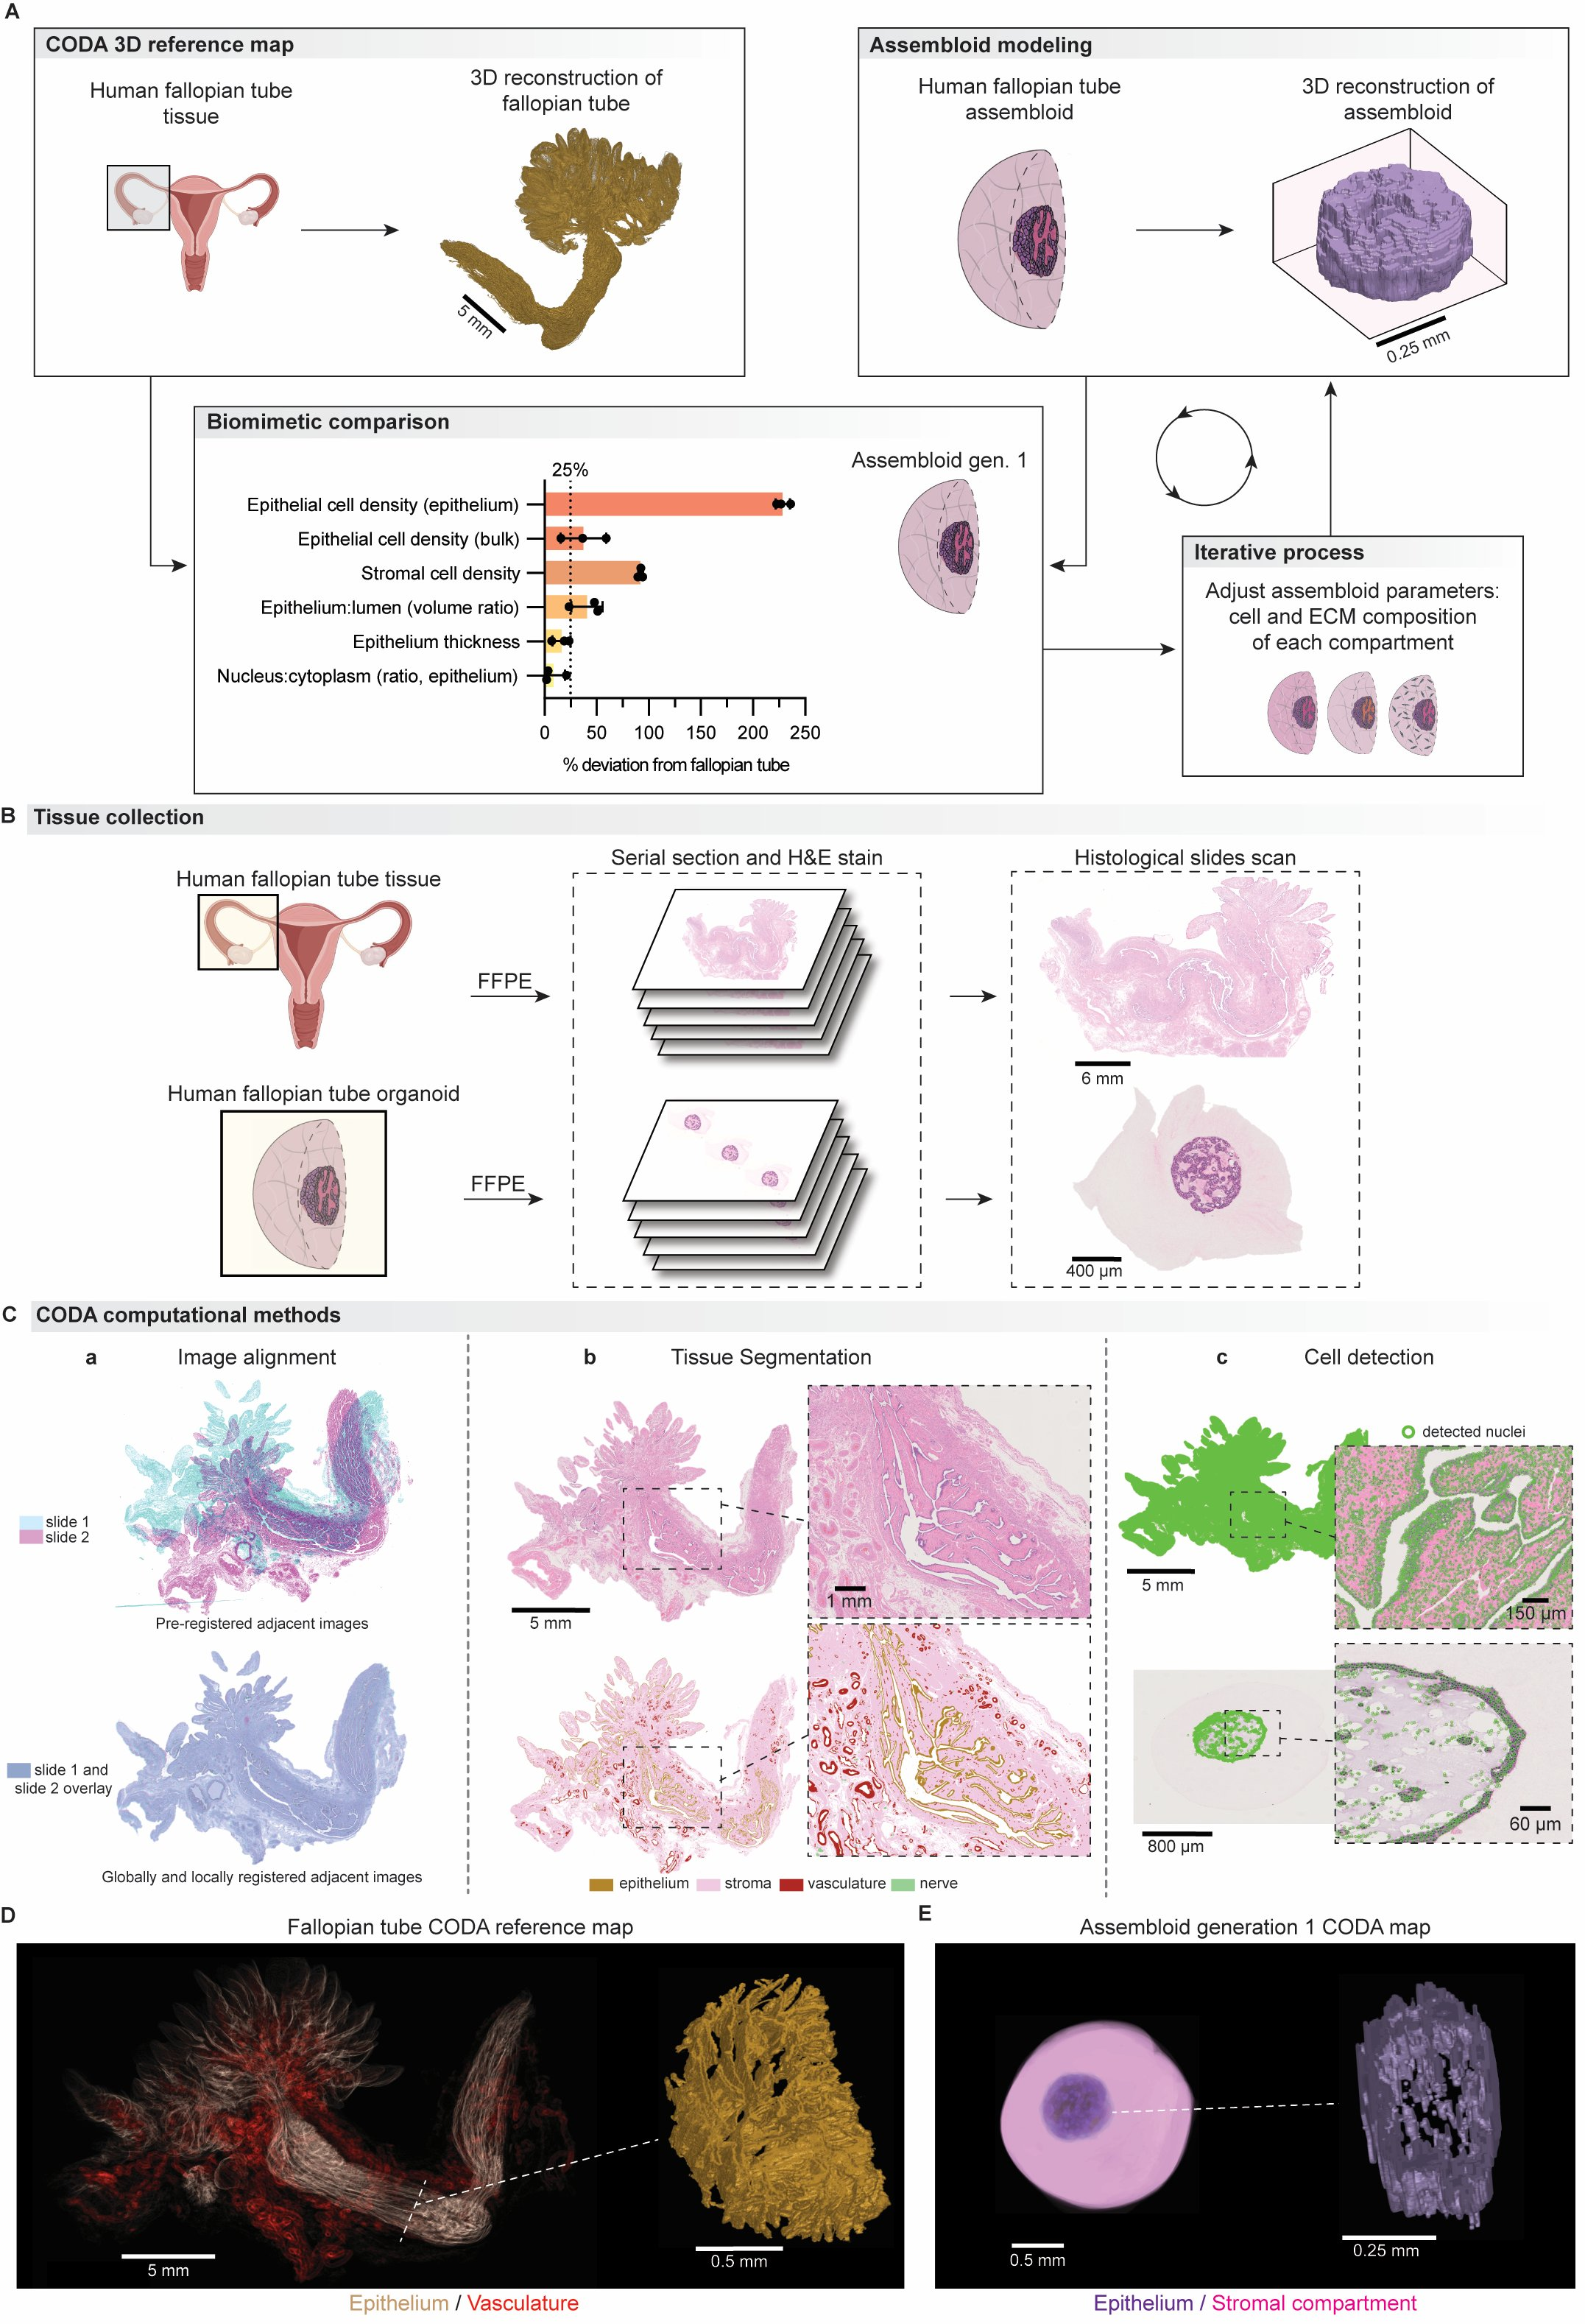
\includegraphics[width=1\textwidth,height=0.85\textheight,keepaspectratio,clip,page=1]{figures/chapter4/fig_5.jpg}
            \captionsetup{font=small}
            \caption{\textbf{Combined CODA and assembloid modeling in tandem produce a tissue-validated assembloid model.} (A) An iterative platform compared a tissue reference map (top left) and assembloid maps (top right). (Bottom left) Architectural quantifications were compared from these maps. (Bottom right) Assembloid parameters were adjusted and CODA imaging repeated until an assembloid generation closely matched the tissue architecture. }
            \label{chapter4_fig5}
        \end{center}
    \end{figure}
    
    \begin{figure}[h!]
        \ContinuedFloat
        \captionsetup{font=small}
        \caption[]{The CODA workflow: (B) Fallopian tube tissue and assembloids were formalin fixed, paraffin embedded (FFPE),  and the entire tissue was serial sectioned. One in every two tissue sections was stained with hematoxylin and eosin (H&E) and scanned at 20X magnification. (C) a, All scanned tissue sections were computationally aligned by an elastic registration process in sequential order. b, Tissue components such as the epithelium (gold), stroma (pink), vasculature (red) and nerves (green) were manually annotated in a small fraction of the images to train the deep learning algorithm to automatically segment all tissue sections. c, Individual cell nuclei were detected from the H&E images. Noise from image scans was adjusted in the cell count. (D) Z-projection of fallopian tube epithelium (gold) and vasculature (red) from a reference map. Scale bar, 5 mm. A 3D reconstruction of a cross section of the fallopian tube is shown (right). Scale bar, 0.5 mm. (E) Z-projection of the assembloid epithelium (purple) and stroma-like region (pink) from an assembloid map. Multi-compartment assembloid parameters: 1 x 104 FTECs in a growth factor reduced Matrigel core, 2 mg/mL collagen I corona. Scale bar, 0.5 mm. A 3D reconstruction of the assembloid epithelium is shown (right). Scale bar, 0.25 mm.}
    \end{figure}

    \begin{figure}[p]
        \begin{center}
            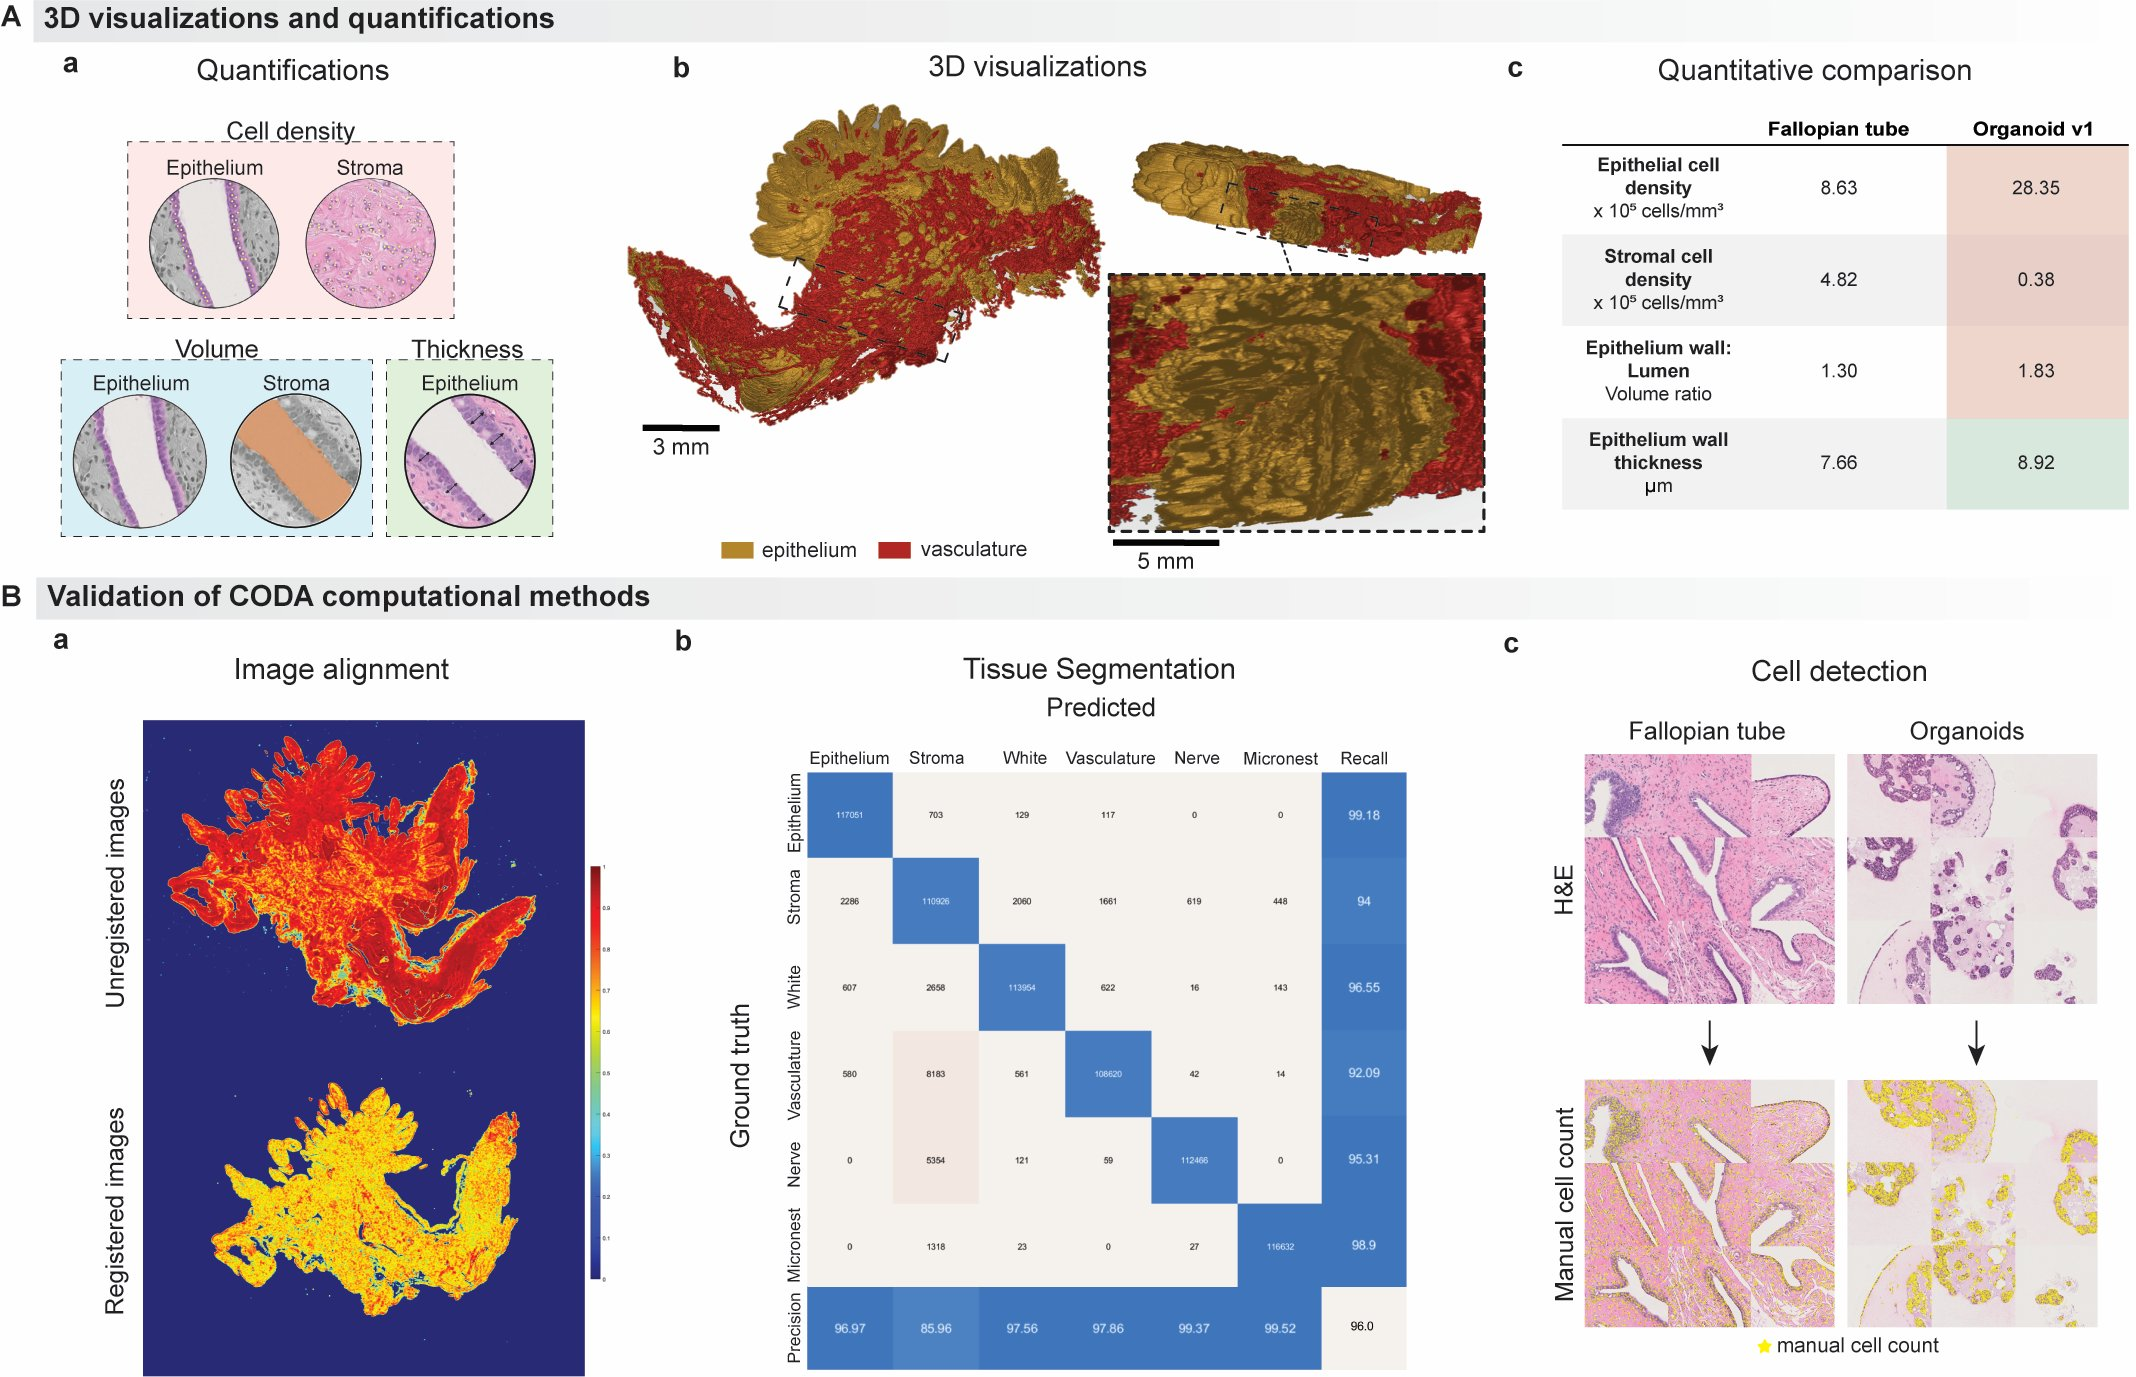
\includegraphics[width=1\textwidth,height=0.85\textheight,keepaspectratio,clip,page=1]{figures/chapter4/fig_S5.jpg}
            \captionsetup{font=small}
            \caption{\textbf{CODA post-processing.} (A) a, An array of tissue quantifications was measured from the processed tissue sections, and b, fallopian tube tissue and assembloids were visualized in 3D. Shown is an epithelium (gold) and vasculature (red) map of the fallopian tube. c, Architectural quantifications from each assembloid generation were compared to the tissue. (B) Independent testing of the CODA computational methods validated the performance of our reference maps, including a, image alignment, b, tissue segmentation, and c, cell detection.}
            \label{chapter4_figS5}
        \end{center}
    \end{figure}
    
    
    \subsection{Iterative changes to assembloid parameters converge towards a next-generation assembloid that mimics the fallopian tube architecture}
    CODA is a high resolution 3D tissue mapping technique, which we use here to improve our assembloid model; however, CODA is expensive, time-intensive, and requires specialized computational tools, making the technique medium throughput. To best leverage the insights gained from CODA maps, we chose seven different combinations of assembloid parameters including epithelial cell seeding densities, core Matrigel compositions, and corona collagen densities in addition to the standard organoid model (Fig. 6A, fig. S6A). These assembloids were not stimulated with β-estradiol to best reflect the post-menopausal conditions of the reference fallopian tube donor, where estrogen levels are low\cite{brodowska2021a,elmlinger2002a,andrew2022a} and fewer epithelial cells are ciliated\cite{crow1994a,donnez1985a,brodowska2021a}. Beginning with (1) the original assembloid parameters (1 x 10$^4$ epithelial cells seeded in a growth factor reduced Matrigel core and embedded in a 2 mg/mL collagen I corona), we first increased the collagen density in the assembloid corona (2) to 4 mg/mL and 6 mg/mL. Increasing the collagen density reduced the effect of epithelial cell contractility on shrinking the total size of the assembloid core, but did not significantly change the epithelial structure within the assembloid (Fig. 6A). We similarly changed the composition of the assembloid core ECM by seeding epithelial cells in a Matrigel matrix containing growth factors (3). This adjustment led to a change in the epithelial architecture where epithelial structures remained less connected within the assembloid core, as visualized by confocal microscopy. A similar difference in assembloid architecture was also observed when (4) decreasing the epithelial seeding in the assembloid core (5 x 10$^3$ cells seeded in a growth factor reduced Matrigel core and 2 mg/mL collagen corona) where the interconnected mucosal folding architecture again appeared less mature. 
    A unique advantage of the multi-compartment assembloid is that stromal cells can be added into the collagen-dense stroma-simulating corona (Fig. 6B). With this modification, we observed significant ECM remodeling when stromal cells were seeded in a 2 mg/mL collagen I corona, so we also increased the collagen concentration to 6 mg/mL (Fig. 6A, parameter modification 5). The standard organoid technique (6) was also imaged using CODA for a total of eight models that were analyzed using our architectural validation platform. Computational analysis was blinded to these experimental conditions.
    An array of structural quantifications were obtained from each assembloid map and compared to the CODA quantifications of the whole fallopian tube (Fig. 6C, fig. S6B). The measurements from this fallopian tube reference map focused on the ampulla region near the fimbriated end where a defined volume could be measured. This platform can be adjusted, however, to focus on different tissue regions and different arrays of architectural quantifications specific to the study. The epithelial and stromal cell seeding densities are two parameters of the assembloids that are easily adjusted, but have different impacts on the assembloid architecture. Cell density was calculated as a bulk measurement (epithelial cell count normalized by total assembloid volume) and as a packing density (epithelial cell count normalized by epithelial volume). While the epithelium cell density differed significantly from the reference tissue for all assembloid models when calculated as a packing density within only the organ/assembloid epithelium (Fig. 6D), the epithelial bulk cell density calculated across the whole assembloid more closely matched the tissue epithelial bulk density (Fig. 6E). 
    The inclusion of stromal cells had a significant impact on assembloid similarity to the tissue (Fig. 6F), which highlights the necessity of compartmentalization in an assembloid. Stromal cells can only be accurately incorporated into a fallopian tube assembloid model when they are adjacent to the epithelium and in direct contact with a collagen I matrix different from the epithelial ECM\cite{lengyel2022a}. Stromal cells were seeded at a ratio of 6 stromal cells to every 10 epithelial cells (6 x 10$^3$ stromal cells in the corona and 1 x 10$^4$ epithelial cells in the core). This seeding ratio accounted for the different proliferation rates of the cell types so that the final ratio of stromal cells to epithelial cells in mature assembloids closely matched the ratio counted in the tissue reference map (fig. S6B). The final number of stromal cells in mature assembloids was further modulated by collagen density in the corona. By increasing the collagen density from 2 mg/mL to 6 mg/mL, we decreased the final stromal cell count, which ultimately decreased the similarity of the stromal cell density per mm$^3$ total volume of our assembloid to the stromal cell density of the tissue within a 1 mm$^3$ region surrounding the fallopian tube lumen (Fig. 6F). Incorporating stromal cells into the assembloid corona also limited the proliferation of the assembloid epithelium (fig. S6C). 
    Additional quantifications included the epithelial wall volume and lumen volume, which was reported as a ratio to demonstrate the similarity of the relative scale of the assembloid to the relative scale of the reference fallopian tube (Fig. 6G). We also measured the thickness of the epithelium wall, which is an indicator of cellular organization (Fig. 6H). As shown in Fig. 6C, the fallopian tube epithelium can be a mixture of monolayered regions and regions where the epithelium becomes multi-layered. Here, we determined the average epithelium thickness across the whole organ epithelium and confirmed that the assembloid epithelium organized similarly. Finally, the nucleus to cytoplasm ratio of epithelial cells was measured so that we could compare the intracellular dimensions of epithelial cells to ensure these cells were not overpacking in the assembloid core (Fig. 6I).
    These quantifications for each assembloid generation were compared to the values for the reference fallopian tube by principal component analysis (PCA) (Fig. 6J). Each data point in the PCA plot represents a consolidation of multiple architectural quantifications derived from our CODA analysis, including epithelial and stromal cell densities, epithelial wall and lumen volume ratios, epithelium thickness, and nucleus to cytoplasm ratios presented above (Fig. 6D-I). This approach allows us to compare the structural similarity across different assembloid conditions and with the reference human fallopian tube tissue while simultaneously considering multiple parameters. The detailed measurements for each architectural feature used in this analysis are presented in Fig. S6B (Data S8), providing a comprehensive view of the data underlying each point in the PCA plot. PC1 and PC2 explained 34.75\% and 30.06\% of the total variance, respectively (PC3: 16.45\%, PC4: 12.72\%, PC5: 4.74\%, PC6: 1.28\%). This analysis revealed that the combination of seeding 1 x 104 FTECs in a growth factor reduced Matrigel core and embedding that core in a 2 mg/mL collagen I corona with 6 x 10$^3$ stromal cells (1 x 10$^4$ 2 mg/mL + S) best mimicked the reference fallopian tube tissue. The 1 x 10$^4$ 2 mg/mL + S condition stood apart from all other generations of the multi-compartment and standard organoid as a more accurate approximation of the fallopian tube architecture. The deviation between this assembloid and the reference fallopian tube was < 25\% for four of six architectural quantifications (Fig. 6F-I), thus this generation of multi-compartment assembloid achieved the target similarity to the reference fallopian tube. Finally, Euclidean distance analysis (fig. S6D), which gives equal weight to all metrics, also agreed that the similarity of the 1 x 10$^4$ 2 mg/mL + S condition to the reference fallopian tube was significantly improved compared to all other tested assembloid generations. The most distinguishing quantification was the stromal cell packing density, which was significantly improved in this assembloid generation. All assembloid parameters (1 x 10$^4$ epithelial cells seeded in growth factor reduced Matrigel with a 2 mg/mL collagen stroma) matched our molecularly and functionally validated assembloids with the only new addition of stromal cells into the corona. Via fluorescence confocal microscopy, we visualized in greater detail the architecture of this final assembloid generation (Fig. 6K, fig. S6E). Intricate epithelial folding mimicking the architecture of the fallopian tube mucosa was observed throughout the assembloid with a surrounding but distinct stroma-like region (Fig. 6L).
    
    \begin{figure}[p]
        \begin{center}
            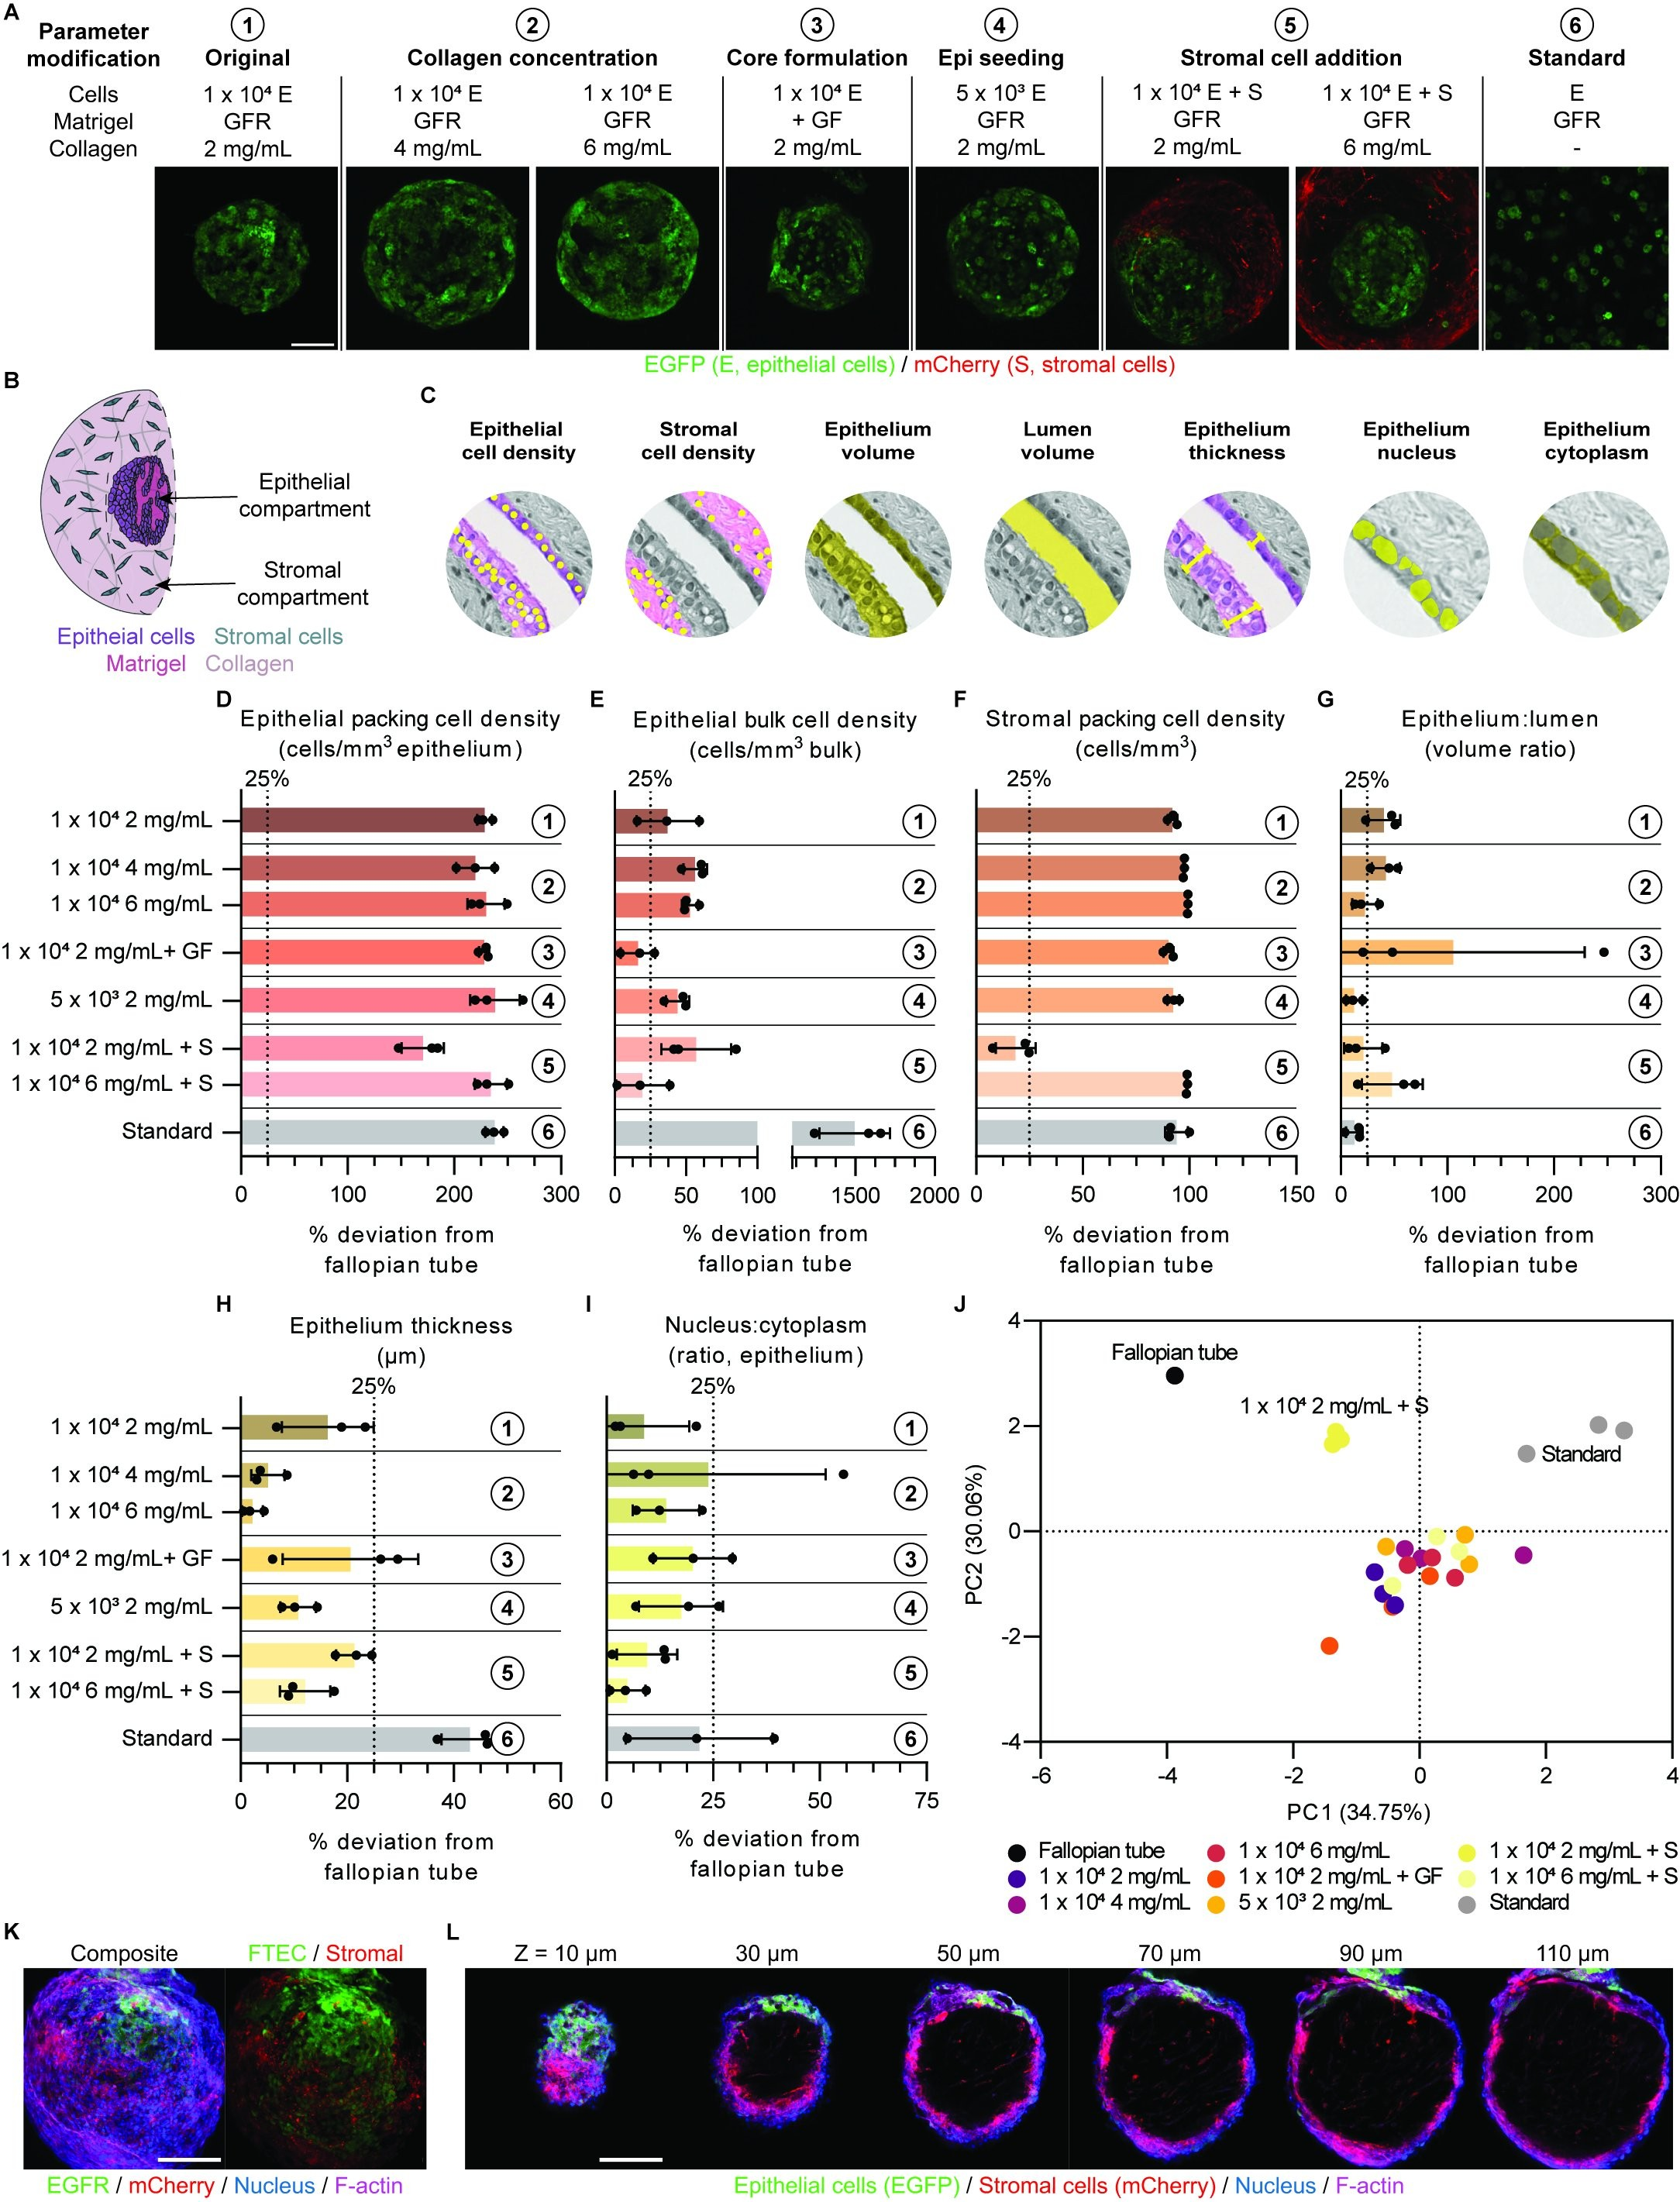
\includegraphics[width=1\textwidth,height=0.85\textheight,keepaspectratio,clip,page=1]{figures/chapter4/fig_6.jpg}
            \captionsetup{font=small}
            \caption{\textbf{Iterative changes to assembloid parameters produces a model that mimics the fallopian tube.} (A) Cell seeding numbers (1 x 10$^4$ or 5 x 10$^3$ cells/core), cell types (E = FTECs, S = stromal cells), Matrigel type (GFR = growth factor reduced, +GF = formulation with growth factors), and collagen density (2, 4, or 6 mg/mL) were adjusted in the multi-compartment model. Lines indicate a new parameter modification. Images are maximum intensity projections of stacks of fluorescence confocal microscopy images. EGFP-tagged FTECs (green) and mCherry-tagged stromal cells (red). Scale bar, 300 µm.}
            \label{chapter4_fig6}
        \end{center}
    \end{figure}
    
    \begin{figure}[h!]
        \ContinuedFloat
        \captionsetup{font=small}
        \caption[]{(B) Representative cartoon of the compartmentalization of epithelium and stroma within an assembloid. Epithelial cells (purple), stromal cells (blue), Matrigel (magenta), and collagen (pink). (C) Depictions of the architectural quantifications from CODA maps. The percent deviation of each assembloid generation from the fallopian tube reference values: (D) epithelial packing density within the epithelium wall only (cells/mm$^3$ epithelium), (E) epithelial bulk cell density across the whole tissue/assembloid (cells/mm$^3$ bulk), (F) stromal cell packing density within the stroma only (cells/mm3), (G) volume ratio of epithelium wall to lumen, (H) epithelium wall thickness (µm), and (I) ratio of epithelium nucleus to cytoplasm. Lines and numbering coordinate with parameter modifications. Dotted line indicates maximum target deviation (25\%). n = 3. Data are mean ± SD. (J) Quantitative comparison of assembloids to the healthy fallopian tube via PCA. Principal component \% proportion of variance listed. n = 3. (K) Maximum intensity projections of stacks of confocal fluorescence microscopy images of the 1 x 10$^4$ 2 mg/mL + S assembloid generation. FTEC (green), stromal cells (red), nuclear DNA (blue), F-actin (magenta). Scale bar, 200 µm. (L) Confocal fluorescence microscopy images of the 1 x 10$^4$ 2 mg/mL + S assembloid generation at varying heights throughout the assembloid. FTEC (green), stromal cells (red), nuclear DNA (blue), F-actin (magenta). Scale bar, 200 µm.}
    \end{figure}

    % \clearpage
    \FloatBarrier
    \subsection{Discussion}
    
    We demonstrate a tissue-informed assembloid engineering platform for the development and validation of in vitro models of organs with quantitative comparisons between the assembloid and the reference cellular map of the organ of interest. This multifaceted experimental, proteomics, and computational-based protocol can be applied to organoid/assembloid models of any tissue/organ and adapted to match the architectural, molecular, and functional parameters of the organ of interest. CODA-based analysis paired with multi-compartment assembloid modeling forms a robust platform that develops custom physiologically and anatomically accurate in vitro models. This platform enables the detailed study of the intricacies of many diseases and conditions. 
    This platform is demonstrated in the context of a healthy human fallopian tube as a basis for future studies of  gynecological conditions and diseases, such as HGSC and ectopic pregnancy\cite{shao2010a,chua2017a,labidi-galy2017a,jones2013a,kim2018a,ducie2017a}. We first demonstrated the structural similarity of our multi-compartment assembloid to the mucosal folding and ECM composition of the human fallopian tube following protocols that were previously used to validate the current state-of-the-art fallopian tube organoid model\cite{kessler2015a,xie2018a}. Second, the molecular similarity of our assembloid model to the fallopian tube was evaluated via comprehensive DIA-MS proteomics\cite{gillet2012a,collins2017a,bons2023a,meier2020a}. We measured the response of fallopian tube assembloids to female reproductive hormone stimulation via traditional functional assays\cite{kessler2015a,xie2018a,barton2020a} and developed a novel assay that measured the ability of the assembloid epithelium to actively transport an oocyte\cite{croxatto2002a,leese2001a,yuan2021a,suarez2021a,wanggren2008a}. Through these two functional assays, the multi-compartment assembloid mimicked the molecular and mechanical functions of the fallopian tube. Finally, we directly compared the multi-compartment assembloid architecture to a reference fallopian tube using quantitative metrics via CODA\cite{kiemen2022a}. Design parameters of the multi-compartment assembloid were customized to best match the post-menopausal conditions of this reference organ through iterative adjustments to assembloid design parameters and sequential CODA mapping. Through this comprehensive analysis, our multi-compartment assembloid demonstrated physiological similarity to the fallopian tube via molecular, functional, and architectural assessments.
    Customizing an assembloid model with reference to the architecture of a whole, transplantation-quality human organ provides an additional quantitative validation of the assembloid model. To our knowledge, direct 3D and quantitative comparison of in vitro cell culture models to organ microarchitecture and cellular composition has never been performed for fallopian tube or other organoid/assembloid models, although the field of in vitro modeling has recognized the importance of validation through other histopathology and tissue-omics-based approaches\cite{garcia-alonso2021a,camp2018a,zhao2022a}. The complex heterogeneity of tissues can only be revealed in 3D\cite{kiemen2022a,Forjaz2025Three}, hence our prioritization of 3D CODA mapping over conventional histological analysis (2D).
    As parameters of our multi-compartment fallopian tube assembloid were modulated, CODA imaging and architectural quantification identified an optimized combination of assembloid parameters. The epithelial and ECM composition of this optimized assembloid design (1 x 104 epithelial cells seeded in growth factor reduced Matrigel with a 2 mg/mL collagen stroma) matched our initial design parameters that we validated via molecular and functional assays. The importance of a secondary compartment was strengthened by the CODA-based platform identifying the addition of stromal cells in the corona (1 x 10$^4$ seeded in growth factor reduced Matrigel with a 2 mg/mL collagen stroma containing 6 x 10$^3$ stromal cells) as the only modification to these original assembloid design parameters to significantly enhance the accuracy of the fallopian tube assembloid architecture. Stromal cells can only be physiologically added to such assembloid models when isolated from epithelial cells in a collagen-rich ECM, which necessitates a multi-compartment model. While ideally, all structural, molecular, and functional assays would be performed using this optimized version of the assembloid, limitations of the system make the molecular and functional assays difficult to perform in a coculture model. Adding stromal cells to the collagen compartment makes the corona more opaque and more difficult to image at significant depths into the assembloid using light-based microscopy methods. Molecular assessments are complicated by sample loss and loss of 3D cell-cell or cell-ECM interactions when attempting to harvest cell types individually for molecular assays. Our bead displacement assay testing the mechanical function of the fallopian tube epithelium to transport an object was also difficult to perform in the coculture system. Time-lapse imaging of the same location is required, but the whole assembloid shifts significantly when stromal cells are reorganizing the collagen compartment. For these reasons, we relied on the closest approximation to our CODA optimized assembloid parameters (1 x 10$^4$ seeded in growth factor reduced Matrigel with a 2 mg/mL collagen stroma) for our molecular and functional assessments.
    The use of customizable multi-compartment assembloids allows us to decipher some of the key compositional features that support the maturation, controlled growth, and maintenance of fallopian tubes. This work establishes the critical importance of two physiological extracellular matrices (i.e., a basement membrane and surrounding collagen compartment)\cite{wheeler1982a,popescu2005a} for FTECs to organize into mucosal folds and stimulate the production of additional ECM proteins that match the ECM composition of the human fallopian tube\cite{shao2023a}. This ECM composition can introduce a limitation of the multi-compartment assembloid system where the lumen-like region is filled with Matrigel (basement membrane) when the true fallopian tube architecture contains a hollow lumen. However, such physiological cell-ECM interactions are necessary to polarize FTECs such that both ciliated and secretory cells face the lumen-like region\cite{popescu2005a,kessler2015a} where ciliated cells could reproduce the organ’s mechanical function and transport an oocyte\cite{yuan2021a,suarez2021a,wanggren2008a}. We also establish the critical importance of stromal cells in a secondary compartment, as observed in fallopian tube tissue\cite{wheeler1982a}, to limit epithelial growth, so that the mucosal folding architecture could be maintained over long time scales. 
    Our multi-compartment assembloid model of the human fallopian tube is a tissue-validated, healthy model. In future work, the cell-cell and cell-ECM interactions in the assembloid model can also be customized to reflect diseased tissues (e.g., precursor lesions to HGSC\cite{kuhn2012a}) and referenced back to corresponding diseased tissue CODA maps via the iterative platform we demonstrated here.  These studies could include altering the ECM composition\cite{rentchler2019a} and healthy vs. p53 signature cell ratios in the epithelium\cite{shih2021a}, or investigations of cilia-driven transport of developing oocytes in tubal pregnancy\cite{shao2010a,chua2017a}.  Other studies of the role of hormone changes in successful embryo implantation are also possible as HSPG2 and other protein expression levels were tunable through \textbeta-estradiol stimulation in the multi-compartment model\cite{chen2023a,garcia2024a}.  The versatility of this approach provides the opportunity to include additional cell mechanical interactions or introduce disease-related ECM changes in downstream experimental applications, or to apply similar 3D culture, proteomics-based, and CODA mapping techniques to evaluate the physiological accuracy of in vitro models of other human tissues. Through our iterative process, we produced a quantitatively optimized and functional assembloid model of a human fallopian tube. This assembloid validation platform can be applied to any tissue-organoid or tissue-assembloid pair to determine the biological accuracy of in vitro models.
    
    \section{Materials and Methods}
    \subsection{Fallopian tube tissue}
    Whole healthy fallopian tube tissues were received from organ procurement organizations from donors with no history of disease. All procedures were approved by the Johns Hopkins Internal Review Board (IRB00324065). The tissues were transported in saline on wet ice, formalin fixed (10\%, VWR 16004-121) and paraffin embedded. The entire tissue was serial sectioned at 4 µm thickness at Johns Hopkins Oncology Tissue Services (SKCC). Tissue sections were stained with hematoxylin and eosin, or immunohistochemistry (IHC) stained. Antibodies used in IHC staining are listed in table S1. Tissue sections were scanned at 20X or 40X magnification (Hamamatsu NanoZoomer S210).
    
    \subsection{Cell culture}
    Fallopian tube immortalized cells were the FT2821J (epithelial)\cite{park2021a,wang2022a,jung2014a,song2019a}, FT194 (epithelial, CVCL-A4AW)\cite{wang2022a} and hS1 (fibroblast-like stromal)\cite{park2021a} cell lines. Cells were cultured in RPMI 1640 (Gibco 11875-093) with 10\% FBS (Corning 35-010-CV) and 1\% penicillin-streptomycin (Sigma P0781). Fallopian tube primary epithelial cells (LifeLine Cell Technology FC-0081) were validated and quality tested at LifeLine Cell Technology and cultured in complete ReproLifeTM Reproductive Medium (LifeLine Cell Technology LL-0068) for a maximum of 3 passages. All cells were cultured at 37°C and 5\% CO2 in a humidified incubator and did not surpass 20 cell passages. All experiments were conducted using these base culture mediums for immortalized or primary cells.
    Fluorescently tagged cells were transduced via lentivirus delivery of the fluorescent tag. Luciferase expressing cells were transduced via lentivirus delivery of a luciferase-mCherry tag (pSLCAR-CD19-BBz [Addgene 135992] with luciferase [Addgene 46793] and mCherry [Addgene 84020] sequences inserted). Transduced populations were expanded and sorted by fluorescence-activated cell sorting (SONY SH800).
    
    \subsection{Multi-compartment assembloid}
    The protocol for generating multi-compartment assembloids is described in greater detail by Lee, et al., where the protocol was first established as a tumor organoid model\cite{lee2022a}. In short, a single-cell suspension of 1 x 104 or 5 x 103 fallopian tube epithelial cells per µL Matrigel (standard formulation 354234 or growth factor reduced 354230, Corning) were pipetted in 1 µL volumes in columns (USA Scientific 1111-3700) containing mineral oil (Sigma 69794) and allowed to gel at 37°C. After 1 h, these cores were collected in cell culture medium (RPMI 1640, Gibco 11875-093) to wash off the mineral oil and embedded in collagen I (high concentration rat tail type I, Corning 354249). A final concentration of 2, 4 or 6 mg/mL collagen I was used according to a previously described protocol (101–104). Adjustments to the collagen I concentration in the assembloid corona were made to assess the effects of corona composition on assembloid architectural similarity to fallopian tube tissue, or to support longer-term cultures of fallopian tube epithelial cells.  Drops containing one assembloid core and 10 µL of collagen I were pipetted into fresh mineral oil columns and again allowed to gel at 37°C. After 1.5 h, these assembloids were collected in cell culture medium to wash off any remaining mineral oil and plated in a 96-well round bottom plate (Genesee Scientific 25-224) with normal cell culture medium as described above. All assembloids were cultured at 37°C and 5\% CO2 in a humidified incubator. All assembloids were grown for at least 6 days (immortalized FTECs) or 9 days (primary FTECs) to allow time for the epithelial architectures to mature. These multi-compartment assembloids are medium throughput, generating up to 96 assembloids per batch.  The consistency of size control across batches was measured using NIS Elements software.
    
    \subsection{Standard organoid}
    The protocol for generating standard organoid is described in greater detail by Kessler, et al. (28) Briefly, fallopian tube epithelial cells were suspended in growth factor reduced Matrigel (Corning 354230) at 500 cells/µL. 50µL drops of the mixture were plated on a glass bottom plate and allowed to gel. Organoids were grown in organoid formation medium containing Advanced DMEM/F-12 (Gibco 12634010), L-Glutamine (1\%, Gibco 25030081), B-27 (2\%, Gibco 17504044), EGF (0.1 µg/mL, ThermoFisher PHG0311), Y-27632 ROCK Inhibitor (10 µM, Cayman Chemical 10005583), TGF-\textbeta RI Kinase Inhibitor VI SB431542 (0.5 µM, Sigma 616464) and HEPES (1\%, Gibco 15630080). All organoids were cultured at 37°C and 5\% CO2 in a humidified incubator. Timelines used for standard organoids matched the culture timelines of multi-compartment assembloids.
    \subsection{PrestoBlue proliferation assay}
    Assembloid total proliferation was assessed via the PrestoBlue (ThermoFisher A13262) proliferation assay. Assembloids were incubated with PrestoBlue (10X) diluted to 1X in culture medium for 3 h at 37°C and 5\% CO$^2$ in a humidified incubator. Red fluorescence (RFU) was read on a SpectraMax plate reader (Molecular Devices, excitation 540, emission 600, cutoff 590). The average of at least 3 background wells of 1X PrestoBlue diluted in culture medium without assembloids was subtracted from all RFU values. PrestoBlue solution was washed from assembloids by replenishing culture medium twice with DPBS (Corning 21-031-CV) and twice with culture medium, and cultured until the next timepoint at 37°C and 5\% CO2 in a humidified incubator.
    
    \subsection{Imaging}
    Assembloids and organoids were imaged on a Nikon Ti2 microscope (phase-contrast) and a Nikon A1R confocal/Nikon Eclipse Ti inverted microscope (DIC, fluorescence and immunofluorescence confocal). The Nikon Ti2 microscope was equipped with a DS-Qi2 camera and a 10X/0.30 Plan Fluor Ph1 DL objective (Nikon). Temperature and CO$^2$ were controlled with a Tokai Hit stage top incubator. The Nikon A1R confocal/Nikon Eclipse Ti inverted microscope was equipped with a 10X/0.30 DIC L/N1 and 20X/10.75 DIC M/N2 Plan Fluor objective (Nikon), a 10X and 20X DIC slider (Nikon), and a N1 and N2 DIC condenser (Nikon). Temperature and CO$^2$ were controlled with an OKO Labs stage top incubator.
    Fluorescence and immunofluorescence confocal images are maximum intensity projections of z-stacks taken over 200-500 µm height of the assembloid with a 10 µm interval. Assembloids were fixed overnight in 4\% PFA or grown in a glass bottom plate for imaging (EGFP, mCherry). Nuclei were stained with Hoechst 33342 (ThermoFisher H3570) and F-actin was stained with Phalloidin 488 (Invitrogen A12379) or Phalloidin 647 (Invitrogen A22287) for 1 h. The primary and secondary antibodies used in immunofluorescence (IF) imaging are outlined in table S1. For IF studies, assembloids were permeabilized in 0.1\% Triton X-100 (Sigma T9284) in DPBS (Corning 21-031-CV) for 1 h, blocked with 5\% normal goat serum (NGS, Cell Signaling Technology) in DPBS for 3 h, and primary stained overnight in 1\% NGS in DPBS. Assembloids were secondary stained for 3 h in 1\% NGS in DPBS. Assembloids were cleared for 20 minutes in a fructose-glycerol clearing solution (105) (60\% glycerol [JT Baker 2136-03], 2.5M D-fructose [Sigma F0127] in DI water) and imaged in DPBS or clearing solution. 

    \begin{table}[htbp]
        \centering
        \footnotesize % Smaller font for the table
        \renewcommand{\arraystretch}{1.2} % Adjust row height
        \caption{Antibodies used in immunofluorescence (IF), immunohistochemistry (IHC), and western blots (WB).}
        \label{chapter4_table_S1}
        \begin{tabularx}{\textwidth}{l l l l}
            \toprule
            \textbf{Application} & \textbf{Antibody} & \textbf{Company} & \textbf{Product \#} \\
            \midrule
            IF  & E-cadherin                  & Cell Signaling Technology & 3195  \\
            IF  & Ki-67                      & Cell Signaling Technology & 9449  \\
            IF  & PAX8                       & Cell Signaling Technology & 59019 \\
            IF  & MUC16                      & Cell Signaling Technology & 29623 \\
            IF  & Anti-rabbit IgG, Alexa Fluor 568 & Invitrogen        & A-11011 \\
            IF  & Anti-mouse IgG, Alexa Fluor 568  & Invitrogen        & A-11004 \\
            IHC & E-cadherin                  & Cell Signaling Technology & 3195  \\
            IHC & Ki-67                      & Abcam                    & ab16667 \\
            IHC & PAX8                       & Cell Signaling Technology & 28556 \\
            WB  & E-cadherin                  & Cell Signaling Technology & 3195  \\
            WB  & Occludin                   & Cell Signaling Technology & 91131 \\
            WB  & GAPDH                      & Cell Signaling Technology & 2118  \\
            WB  & Anti-rabbit IgG, HRP-linked & Cell Signaling Technology & 7074  \\
            \bottomrule
        \end{tabularx}
    \end{table}
    
    \subsection{Transmission electron microscopy}
    Assembloids were fixed (2.5\% glutaraldehyde, 0.1M sodium cacolydate buffer, 3 mM magnesium chloride in DI water), and imaged via transmission electron microscopy. Images were captured and analyzed with the help of a transmission electron microscopy expert at the Johns Hopkins School of Medicine Microscope Facility.
    
    \subsection{Western blot}
    Protein was extracted from 3D cultures and 2D cells with 2X clear sample buffer (120 mM Tris pH 6.8, 4\% SDS, 20\% glycerol) and 1X protease/phosphatase inhibitor (Cell Signaling Technology 5872). 2D cells were scraped from a 10 cm dish after coating the plate with 2X clear sample buffer. All protein samples were sonicated with a needle probe sonicator (10-15 pulses, VWR Scientific) and denatured at 100°C for 5 minutes. Samples were stored at -80°C. Protein concentration was measured by microBCA (ThermoFisher, 23235) and absorbance measured on a SpectraMax plate reader (Molecular Devices, 562nm). Samples were diluted to 1 µg/µL in 2X Lamelli (BioRad 1610737) and heated for 5 minutes at 100°C. Samples were loaded in a 4-15\% mini-protean gel (BioRad 4561086) for gel electrophoresis (BioRad PowerPac). Protein bands were transferred to a PVDF membrane using a Transblot Turbo pack (BioRad 1704156). The blot was blocked in blotting-grade blocker (5\%, 1706404) in TBST (1X Tris Buffered Saline [BioRad 1706435], 0.1\% Tween 20 [Sigma P1379], in DI water) for 1 h and primary stained overnight at 4°C. HRP-conjugated secondary antibodies were incubated at room temperature for 1 h. Western blots were imaged on a BioRad ChemiDoc XRS+ imager with Prometheus™ ProSignal™ HRP substrate (Genesee Scientific 20-302). Antibodies are listed in table S1. 
    \subsection{Hormone stimulation and RT-qPCR}
    After 7 days of culture, assembloid architecture had matured, and assembloids/organoids were treated with \textbeta-estradiol (E2, 500 pmol/L, Sigma E2758), progesterone (P4, 50 ng/mL, Fisher Scientific AC225650250)\cite{kessler2015a}, or an untreated control. Hormones were diluted in ethanol prior to dilution in culture medium, so this dilution was equivalently reflected in the untreated control. Assembloids and organoids were grown for another 7 days with hormone stimulation before mRNA harvested (Zymo Research R2052 Direct-zol RNA MiniPrep 11-331) and cDNA synthesized using the iScript™ cDNA Synthesis Kit (BioRad 1708891) and a Blue-Ray Biotech thermocycler. Expression of select genes (primers from Integrated DNA Technologies listed in table S2)\cite{kessler2015a,xie2018a,ma2022a,rajurkar2017a,liu2020a} was quantified by iTaq-SYBR Green (BioRad) RT-qPCR on a BioRad CFX384 Touch Real-Time PCR detection system. Relative expression was calculated according to the equations described by Pfaffl\cite{pfaffl2001a}.

    \begin{table}[htbp]
        \centering
        \footnotesize
        \renewcommand{\arraystretch}{1.2}
        \caption{Primers used in RT-qPCR.}
        \label{chapter4_table_S2}
        \begin{tabularx}{\textwidth}{l l X} % X column automatically adjusts width
            \toprule
            \textbf{Gene} & \textbf{FWD/RVS} & \textbf{Sequence} \\
            \midrule
            PAX8   & FWD & AAGTGCAGCAACCATTCAACC \\
            PAX8   & RVS & CTGCTCTGTGAGTCAATGCTTA \\
            FOXJ1  & FWD & GGAGGGGACGTAAATCCCTA \\
            FOXJ1  & RVS & GGTCCCAGTAGTTCCAGCAA \\
            OVGP1  & FWD & TCCCACACATCGTCCAAACAT \\
            OVGP1  & RVS & TCCCCATGATGAGCTTCTCTG \\
            OLFM4  & FWD & ACTGTCCGAATTGACATCATGG \\
            OLFM4  & RVS & TTCTGAGCTTCCACCAAAACTC \\
            MKI67  & FWD & AAGCCCTCCAGCTCCTAGTC \\
            MKI67  & RVS & TCCGAAGCACCACTTCTTCT \\
            TNF    & FWD & CCTCTCTCTAATCAGCCCTCTG \\
            TNF    & RVS & GAGGACCTGGGAGTAGATGAG \\
            ESR1   & FWD & CCCACTCAACAGCGTGTCTC \\
            ESR1   & RVS & CGTCGATTATCTGAATTTGGCCT \\
            PGR    & FWD & ACCCGCCCTATCTCAACTACC \\
            PGR    & RVS & AGGACACCATAATGACAGCCT \\
            18S    & FWD & AGAAGTGACGCAGCCCTCTA \\
            18S    & RVS & GAGGATGAGGTGGAACGTGT \\
            ATUB   & FWD & AGGAGTCCAGATCGGCAATG \\
            ATUB   & RVS & GTCCCCACCACCAATGGTTT \\
            ACTB   & FWD & CATGTACGTTGCTATCCAGGC \\
            ACTB   & RVS & CTCCTTAATGTCACGCACGAT \\
            GAPDH  & FWD & GGAGCGAGATCCCTCCAAAAT \\
            GAPDH  & RVS & GGCTGTTGTCATACTTCTCATGG \\
            RPL13A & FWD & CCTGGAGGAGAAGAGGAAAGAGA \\
            RPL13A & RVS & TTGAGGACCTCTGTGTATTTGTCAA \\
            \bottomrule
        \end{tabularx}
    \end{table}

    \subsection{Bead displacement assay}
    In the bead displacement assay, red fluorescent microbeads (Cospheric FMR-1.3 1-5um) were suspended in Matrigel with FTECs. Both standard organoids and multi-compartment assembloids were generated that contained microbeads only and EGFP-tagged cells with microbeads in the Matrigel. The previously outlined protocols were followed; however, the multi-compartment assembloids were plated in 100 µL collagen I in a flat glass bottom plate so that the same location on an assembloid could be imaged via time-lapse microscopy. Assembloids were treated with \textbeta-estradiol\cite{garcia-alonso2021a} (10 nM, Sigma E2758) or control medium after 24 h. After 7 days of culture, assembloid architecture had matured, and assembloids were imaged via confocal fluorescence microscopy (10X magnification). Time-lapse images were collected every 10 minutes for 12 h. Stage drift was removed from time-lapse images and microbeads tracked across all time points. Microbead trajectories, mean squared displacements and motility information were calculated according to previously published protocols\cite{wu2015a}.
    
    \subsection{Cilia-driven motility assay}
    Multi-compartment assembloids with 10 µL coronas were cultured according to the same specifications of the bead displacement assay (β-estradiol [10 nM, Sigma E2758]\cite{garcia-alonso2021a} treated after 24 h, grown for 7 days to allow assembloid architecture to mature) and digested with 2 mg/mL collagenase I (Gibco 17018029) for 1 h. After digestion, cells were resuspended in DPBS (Corning 21-031-CV) and time-lapse imaged for 1 h (phase-contrast, 10X magnification). After an initial 30 minute incubation to give cells time to settle to the bottom of the plate, cells were imaged for 30 minutes at 1 minute intervals. Individual cells were tracked and their motility parameters calculated according to previously published cell tracking protocols\cite{wu2015a}.
    
    \subsection{Proteomics}
    Multi-compartment assembloids and standard organoids were grown for 18 days, washed 1X with DPBS and stored in cell culture medium for proteomics. The extended 18 day timeline was selected to allow time for the architectures of primary FTEC cultures to mature in the 3D models. The FT2821J FTEC cell line was grown in multi-compartment assembloids with a GFR Matrigel assembloid core and a 2 mg/mL collagen I corona. Primary FTECs were grown in multi-compartment assembloids with a GFR Matrigel assembloid core and a 6 mg/mL collagen I corona, and standard organoids in GFR Matrigel. GFR Matrigel, 2 and 6 mg/mL collagen I controls without cells were also incubated for 18 days with each biological replicate. Multi-compartment assembloids were treated with β-estradiol\cite{garcia-alonso2021a} (10 nM, Sigma E2758) or control medium from day 9 to day 18, with medium refreshed every 3 days.  The number of biological replicates was four for each condition (N = 4), which included 10 or more pooled assembloids/organoids (n = 10+).  For primary cells, two donors were included, and cell culture did not exceed three passages for each donor.
    LC-MS-grade acetonitrile (ACN), methanol and water were obtained from Burdick \& Jackson. Reagents for protein chemistry, including sodium dodecyl sulfate (SDS), triethylammonium bicarbonate (TEAB), trichostatin A, nicotinamide, iodoacetamide (IAA), dithiothreitol (DTT), phosphoric acid, and formic acid (FA), were purchased from Sigma-Aldrich. Urea and phosphate buffered saline (PBS) were purchased from Thermo Fisher Scientific. Sodium chloride was purchased from VWR. Sequencing-grade trypsin was purchased from Promega.
    
    \subsection{Protein digestion and desalting}
    Multi-compartment assembloids and standard organoids and ECM controls were washed twice with cold PBS 1x and then subjected to a lysis buffer containing 8 M urea, 2\% SDS, 200 mM TEAB, pH 8.5, 75 mM NaCl, 1 μM trichostatin A, 3 mM nicotinamide, and 1x protease/phosphatase inhibitor cocktail (Thermo Fisher Scientific, 78442), and incubated overnight at 4°C on a rotator.  Lysates were clarified by spinning at 15,700 x g for 15min at 4°C, and the supernatant containing the soluble proteins was collected. Protein concentrations were determined using a Bicinchoninic Acid Protein (BCA) Assay (Thermo Fisher Scientific, 23225), and subsequently 100 μg of protein from each sample were aliquoted and samples were brought to an equal volume using water. Samples were solubilized with 4\% SDS and 50 mM TEAB at pH 8. Proteins were reduced with 20 mM DTT (10 min at 50°C followed by 10 min at room temperature) and then alkylated with 40 mM IAA (30 min at room temperature in the dark). Samples were acidified with a final concentration of 1.2\% phosphoric acid and diluted with seven volumes S-trap buffer (90\% methanol in 100 mM TEAB, pH 8). Samples were then loaded onto the S-trap mini spin columns (Protifi) and spun at 4,000 x g for 10 seconds. The S-Trap columns were washed with S-Trap buffer twice at 4,000 x g for 10 seconds each. A solution of sequencing grade trypsin in 50 mM TEAB at a 1:25 (w/w) enzyme:protein ratio was then added, and after a 1-h incubation at 47°C, trypsin solution was added again at the same ratio and proteins were digested overnight at 37°C. Peptides were sequentially eluted with 50 mM TEAB (spinning at 1,000 x g for 1 min), 0.5\% FA in water (spinning at 1,000 x g for 1 min), and 50\% ACN in 0.5\% FA (spinning at 4,000 x g for 1 min). After vacuum drying, samples were resuspended in 0.2\% FA in water, desalted with Oasis 10-mg Sorbent Cartridges (Waters). All samples were vacuum dried and resuspended in 0.2\% FA in water at a final concentration of 1 μg/μL. Finally, indexed retention time standard peptides (iRT; Biognosys)\cite{escher2012a} were spiked in the samples according to manufacturer’s instructions.
    
    \subsection{Mass spectrometric analysis}
    Samples (200 ng) were loaded onto EvoTips Pure (Evosep) following manufacturer’s protocol. LC-MS/MS analyses were performed on an Evosep One liquid chromatography system coupled to a timsTOF HT mass spectrometer (Bruker). The solvent system consisted of 0.1\% FA in water (solvent A) and 0.1\% FA in ACN (solvent B). Peptides were eluted on a PepSep C18 analytical column (150 µm x 15 cm, 1.5 µm particle size; Bruker) using the 30 SPD method (44-minute gradient length, 500-nl/min flow rate). A zero-dead volume emitter was installed in the nano-electrospray source (CaptiveSpray source, Bruker Daltonics) and the source parameters were set as follows: capillary voltage 1600 V, dry gas 3 L/min, and dry temperature 180°C. Each sample was acquired in data-independent acquisition (DIA) mode coupled to parallel accumulation serial fragmentation (PASEF) or diaPASEF mode\cite{meier2020a} with 1 survey TIMS MS scan and 24 diaPASEF MS/MS scans per 2.03-second cycle. The dual TIMS analyzer was operated in a 100\% duty cycle with equal accumulation time and ramp time of 75 ms each. For each TIMS MS scan, the ion mobility ranged from 1/K0 = 0.85-1.30 Vs/cm2 and the mass range covered m/z 100-1,700. The diaPASEF scheme was defined as 63 x 15 Th isolation windows from m/z 305.9 to 1,250.9 and covering the ion mobility range 1/K0 = 0.74-1.30 Vs/cm2 (Data S1). The collision energy was defined as a linear function of mobility starting from 20 eV at 1/K0 = 0.6 Vs/cm2 to 59 eV at 1/K0 = 1.6 Vs/cm$^2$. For calibration of ion mobility dimension, three ions of Agilent ESI-Low Tuning Mix ions were selected (m/z [Th], 1/K0 [Th]: 622.0289, 0.9915; 922.0097, 1.1986; 1221.9906, 1.13934).
    
    \subsection{DIA-MS data processing with Spectronaut v17}
    All DIA data was processed in Spectronaut version 17.6.230428.55965 (Biognosys) using directDIA. Data was searched against the Homo sapiens proteome with 20,423 protein entries (UniProtKB-SwissProt), accessed on 06/30/2023. Trypsin/P was set as digestion enzyme and two missed cleavages were allowed. Cysteine carbamidomethylation was set as fixed modification, and methionine oxidation and protein N-terminus acetylation as variable modifications. Data extraction parameters were selected as dynamic, and non-linear iRT calibration with precision iRT was selected. Identification was performed using a 1\% precursor and protein q-value, and iRT profiling was selected. Quantification was based on the MS/MS peak area of the 3-6 best fragment ions per precursor ion, peptide abundances were obtained by summing precursor abundances and protein abundances by summing peptide abundances. Interference correction was selected and local normalization was applied. Finally, protein groups were required with at least two unique peptides (Data S2-S7). Differential protein abundance analysis was performed using unpaired t-test, and p-values were corrected for multiple testing, specifically applying group-wise testing corrections using the Storey method (111, 112). For differential analysis, protein groups with q-value ≤ 0.05 and absolute log2(fold-change) ≥ 0.2 were considered to be significantly altered (Data S3-S4).
    
    \subsection{LOPIT organellar protein distribution}
    The hyperLOPIT2015 u2os dataset was downloaded in R (version 4.0.2; RStudio, version 2022.07.0+548) using the pRolocData R package (Bioconductor) and plotted with the pRoloc R package (55, 113). To create the LOPIT organellar protein distribution dataset, a crude membrane preparation from a U2OS cell lysate was fractionated by density gradient ultracentrifugation to separate and enrich organelles based on density\cite{thul1979a,dunkley2004a,mulvey2017a}. Proteins were identified via quantitative multiplexed mass spectrometry and assigned to organelles based on similarities in distribution in the density gradient to well-annotated organelle protein markers. The t-SNE machine learning algorithm was used to reduce the number of dimensions in the LOPIT proteomic data to a 2D map where proteins cluster by similarity from multiple experimental factors\cite{meier2020a}. All LOPIT protein assignments were used as originally determined and without additional refinement.
    
    \subsection{Over-representation analysis}
    Gene Ontology\cite{} (52, 53) biological processes that were upregulated and downregulated following \textbeta-estradiol stimulation were identified by ConsensusPathDB\cite{kamburov2009a,kamburov2011a} over-representation analysis with p-value < 0.01 and Gene Ontology biological process level ≥ 4. The plotted protein ratio is the corrected ratio of the count of proteins mapped to each term divided by the effective size of the dataset.
    
    \subsection{CODA tissue mapping}
    The CODA protocol is described in greater detail by Kiemen et al.\cite{kiemen2022a}. Assembloids that were grown for 10 days so that the architecture could mature and fallopian tube tissues within 12 h of collection were formalin fixed (10\%, VWR 16004-121) and paraffin embedded, then serial sectioned across the whole tissue at 4 µm section thickness. One in every two tissue slides was designated for H\&E staining, while the remaining unstained slides were stored for potential application of multiplexing techniques, such as immunofluorescence, immunohistochemical, and tissue-omics. All subsequent steps were performed by a trainee who was unfamiliar with the experimental design, thus blinding the computational analysis to experimental conditions. Stained slides were scanned at 20X magnification offering a 0.5 micron resolution on the x and y dimensions. To align the H\&E images, a combination of global and nonlinear techniques was implemented in all images in a sample. To statistically measure the similarity between two serially aligned H\&E images, cross-correlation was used. In order to identify individual cells on the H\&E-stained samples, a color deconvolution step was added which extracted the hematoxylin channel of each image, and specific sized and spatially distanced two-dimensional minima were marked as nuclei. A deep learning model was trained on an image subset using manually annotated tissue cases. To enhance the performance of the convolutional neural network on unseen data, data augmentation techniques were integrated, allowing for hue, rotation, and scale changes to the training dataset. The validation of the model was ensured using independent testing images, not used for training, with the mean testing accuracies surpassing ninety percent for true positive segmentation values. Combination of the alignment, semantic segmentation and cell detection computational methods resulted in three dimensional maps of each individual tissue label at single cell resolution. Three-dimensional renderings were performed at 4 µm and 1 µm in x and y dimensions for the whole human fallopian tube and each individual assembloid, respectively. Lastly, three-dimensional analysis of the human fallopian tube and assembloids were performed in isotropic dimensions 4x4x4 µm$3^$.

    \clearpage
    
    \printbibliography[heading=subbibliography, title={References}]
\end{refsection}
% \include{10-chapter-5}




%%%%%%%%%%%%%%%%%%%%%%%%%%% END MAIN MATTER %%%%%%%%%%%%%%%%%%%%%%%%%%%%



%%%%%%%%%%%%%%%%%%%%%%%%%%%%% BACK MATTER %%%%%%%%%%%%%%%%%%%%%%%%%%%%%%

%%%% BIBLIOGRAPHIC REFERENCES
\BibTextSpacing                         % text spacing for each bib item
\fancyhead[L]{\nouppercase \leftmark}
\printbibliography[title={Bibliographic references},
    heading=bibintoc, notcategory=mypapers]
\clearpage     

%%%%%%%%%%%%%%%%%%%%%%%%%    CV     %%%%%%%%%%%%%%%%%%%%
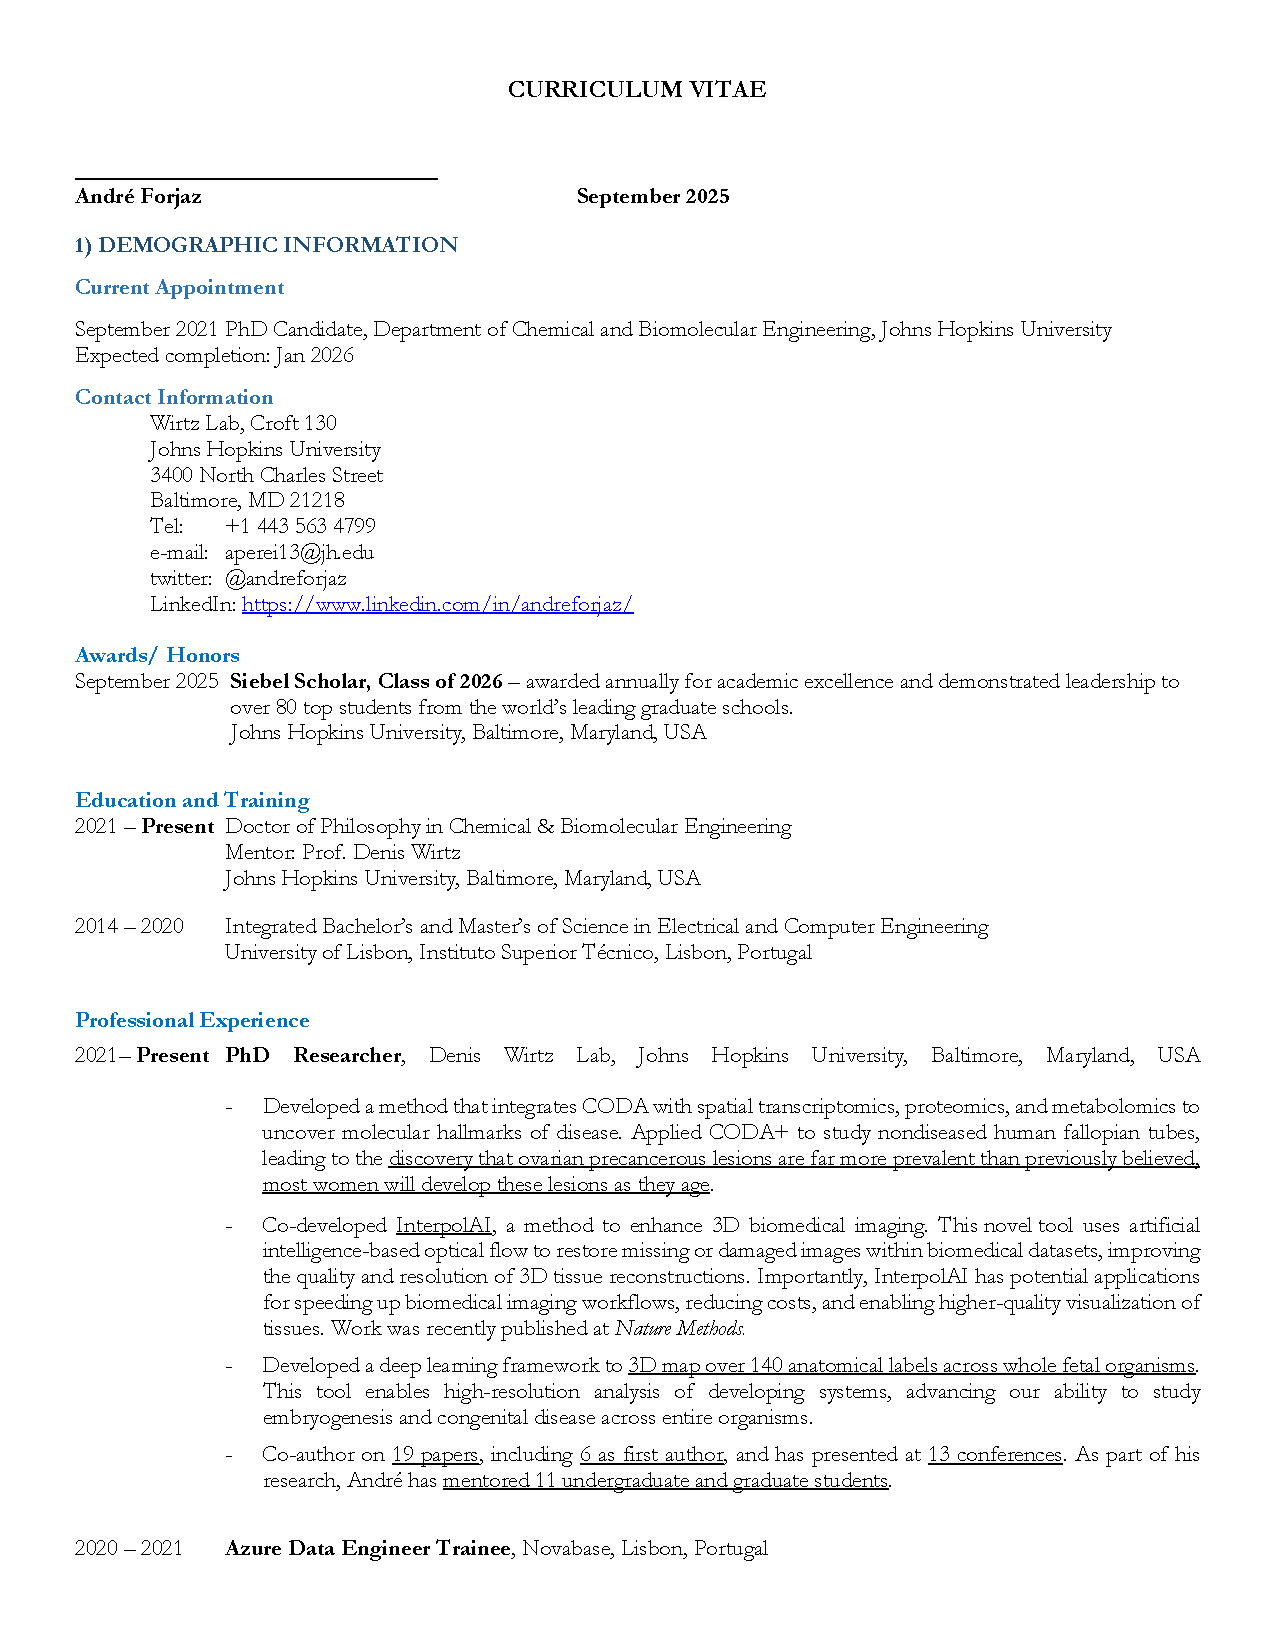
\includepdf[pages=-]{CV_9_27_2025.pdf} % Include all pages from the PDF%% add more main text technical chapters if you have

%%%% Appendix chapter (same header format as the main chapters)
%% if you do not have appendix chapters, then comment them out
% \MainTextSpacing                    
% \fancyhead[L]{\appendixname\ \thechapter. \nouppercase \leftmark}


% \include{11-appendix-A}
% \include{12-appendix-B}

%% add more appendix chapters if you have 

%%%%%%%%%%%%%%%%%%%%%%%%%%% END BACK MATTER %%%%%%%%%%%%%%%%%%%%%%%%%%%%

\end{document}

%%%%%%%%%%%%%%%%%%%%%%%%% DOCUMENT ENDS HERE %%%%%%%%%%%%%%%%%%%%%%%%%%%